\documentclass[twoside]{book}

% Packages required by doxygen
\usepackage{fixltx2e}
\usepackage{calc}
\usepackage{doxygen}
\usepackage[export]{adjustbox} % also loads graphicx
\usepackage{graphicx}
\usepackage[utf8]{inputenc}
\usepackage{makeidx}
\usepackage{multicol}
\usepackage{multirow}
\PassOptionsToPackage{warn}{textcomp}
\usepackage{textcomp}
\usepackage[nointegrals]{wasysym}
\usepackage[table]{xcolor}

% Font selection
\usepackage[T1]{fontenc}
\usepackage[scaled=.90]{helvet}
\usepackage{courier}
\usepackage{amssymb}
\usepackage{sectsty}
\renewcommand{\familydefault}{\sfdefault}
\allsectionsfont{%
  \fontseries{bc}\selectfont%
  \color{darkgray}%
}
\renewcommand{\DoxyLabelFont}{%
  \fontseries{bc}\selectfont%
  \color{darkgray}%
}
\newcommand{\+}{\discretionary{\mbox{\scriptsize$\hookleftarrow$}}{}{}}

% Page & text layout
\usepackage{geometry}
\geometry{%
  a4paper,%
  top=2.5cm,%
  bottom=2.5cm,%
  left=2.5cm,%
  right=2.5cm%
}
\tolerance=750
\hfuzz=15pt
\hbadness=750
\setlength{\emergencystretch}{15pt}
\setlength{\parindent}{0cm}
\setlength{\parskip}{0.2cm}
\makeatletter
\renewcommand{\paragraph}{%
  \@startsection{paragraph}{4}{0ex}{-1.0ex}{1.0ex}{%
    \normalfont\normalsize\bfseries\SS@parafont%
  }%
}
\renewcommand{\subparagraph}{%
  \@startsection{subparagraph}{5}{0ex}{-1.0ex}{1.0ex}{%
    \normalfont\normalsize\bfseries\SS@subparafont%
  }%
}
\makeatother

% Headers & footers
\usepackage{fancyhdr}
\pagestyle{fancyplain}
\fancyhead[LE]{\fancyplain{}{\bfseries\thepage}}
\fancyhead[CE]{\fancyplain{}{}}
\fancyhead[RE]{\fancyplain{}{\bfseries\leftmark}}
\fancyhead[LO]{\fancyplain{}{\bfseries\rightmark}}
\fancyhead[CO]{\fancyplain{}{}}
\fancyhead[RO]{\fancyplain{}{\bfseries\thepage}}
\fancyfoot[LE]{\fancyplain{}{}}
\fancyfoot[CE]{\fancyplain{}{}}
\fancyfoot[RE]{\fancyplain{}{\bfseries\scriptsize Generated on Wed Oct 21 2015 17\+:46\+:53 for Pacman by Doxygen }}
\fancyfoot[LO]{\fancyplain{}{\bfseries\scriptsize Generated on Wed Oct 21 2015 17\+:46\+:53 for Pacman by Doxygen }}
\fancyfoot[CO]{\fancyplain{}{}}
\fancyfoot[RO]{\fancyplain{}{}}
\renewcommand{\footrulewidth}{0.4pt}
\renewcommand{\chaptermark}[1]{%
  \markboth{#1}{}%
}
\renewcommand{\sectionmark}[1]{%
  \markright{\thesection\ #1}%
}

% Indices & bibliography
\usepackage{natbib}
\usepackage[titles]{tocloft}
\setcounter{tocdepth}{3}
\setcounter{secnumdepth}{5}
\makeindex

% Hyperlinks (required, but should be loaded last)
\usepackage{ifpdf}
\ifpdf
  \usepackage[pdftex,pagebackref=true]{hyperref}
\else
  \usepackage[ps2pdf,pagebackref=true]{hyperref}
\fi
\hypersetup{%
  colorlinks=true,%
  linkcolor=blue,%
  citecolor=blue,%
  unicode%
}

% Custom commands
\newcommand{\clearemptydoublepage}{%
  \newpage{\pagestyle{empty}\cleardoublepage}%
}


%===== C O N T E N T S =====

\begin{document}

% Titlepage & ToC
\hypersetup{pageanchor=false,
             bookmarks=true,
             bookmarksnumbered=true,
             pdfencoding=unicode
            }
\pagenumbering{roman}
\begin{titlepage}
\vspace*{7cm}
\begin{center}%
{\Large Pacman }\\
\vspace*{1cm}
{\large Generated by Doxygen 1.8.10}\\
\vspace*{0.5cm}
{\small Wed Oct 21 2015 17:46:53}\\
\end{center}
\end{titlepage}
\clearemptydoublepage
\tableofcontents
\clearemptydoublepage
\pagenumbering{arabic}
\hypersetup{pageanchor=true}

%--- Begin generated contents ---
\chapter{Documentation de Pacman}
\label{index}\hypertarget{index}{}\hypertarget{index_to_do}{}\section{To Do}\label{index_to_do}

\begin{DoxyItemize}
\item La classe \hyperlink{class_game}{Game} ne gère pas encore le passage d\textquotesingle{}un niveau à l\textquotesingle{}autre.
\item La classe \hyperlink{class_game}{Game} ne gère pas encore le son.
\item La classe \hyperlink{class_game}{Game} ne dispose pas encore de toutes les animations.
\item La classe \hyperlink{class_game}{Game} ne dispose pas encore de la table de correspondance des textures. 
\end{DoxyItemize}
\chapter{Hierarchical Index}
\section{Class Hierarchy}
This inheritance list is sorted roughly, but not completely, alphabetically\+:\begin{DoxyCompactList}
\item \contentsline{section}{Double\+Position}{\pageref{class_double_position}}{}
\item \contentsline{section}{Firework}{\pageref{class_firework}}{}
\item \contentsline{section}{Ghost\+Timer}{\pageref{class_ghost_timer}}{}
\item \contentsline{section}{Grid}{\pageref{class_grid}}{}
\item Q\+Object\begin{DoxyCompactList}
\item \contentsline{section}{Arduino\+Handler}{\pageref{class_arduino_handler}}{}
\item \contentsline{section}{Game}{\pageref{class_game}}{}
\item \contentsline{section}{Level}{\pageref{class_level}}{}
\item \contentsline{section}{Pacman\+Unit}{\pageref{class_pacman_unit}}{}
\end{DoxyCompactList}
\item Q\+Widget\begin{DoxyCompactList}
\item \contentsline{section}{Pacscreen}{\pageref{class_pacscreen}}{}
\end{DoxyCompactList}
\item \contentsline{section}{Texture\+Handler}{\pageref{class_texture_handler}}{}
\item \contentsline{section}{Unit}{\pageref{class_unit}}{}
\begin{DoxyCompactList}
\item \contentsline{section}{Ghost}{\pageref{class_ghost}}{}
\item \contentsline{section}{Pacman\+Unit}{\pageref{class_pacman_unit}}{}
\end{DoxyCompactList}
\end{DoxyCompactList}

\chapter{Class Index}
\section{Class List}
Here are the classes, structs, unions and interfaces with brief descriptions\+:\begin{DoxyCompactList}
\item\contentsline{section}{\hyperlink{class_editor_game}{Editor\+Game} \\*La classe \hyperlink{class_editor_game}{Editor\+Game} gère l\textquotesingle{}ensemble des paramètres pouvant être passés au programme Pacman }{\pageref{class_editor_game}}{}
\item\contentsline{section}{\hyperlink{class_editor_level}{Editor\+Level} \\*La classe \hyperlink{class_editor_level}{Editor\+Level} permet de paramétrer un niveau dans Pacman }{\pageref{class_editor_level}}{}
\item\contentsline{section}{\hyperlink{class_editor_unit}{Editor\+Unit} \\*Petite classe graphique permettant de bouger un pion }{\pageref{class_editor_unit}}{}
\item\contentsline{section}{\hyperlink{class_ghost_timer}{Ghost\+Timer} \\*Classe de Timer pour les modes des fantômes }{\pageref{class_ghost_timer}}{}
\item\contentsline{section}{\hyperlink{class_main_window}{Main\+Window} \\*Classe principale graphique }{\pageref{class_main_window}}{}
\item\contentsline{section}{\hyperlink{class_map}{Map} \\*Objet graphique détectant les clics souris et générant des signaux }{\pageref{class_map}}{}
\item\contentsline{section}{\hyperlink{class_new_ghost_mode_dialog}{New\+Ghost\+Mode\+Dialog} \\*Classe graphique de fenêtre pour l\textquotesingle{}ajout d\textquotesingle{}un nouveau mode de poursuite }{\pageref{class_new_ghost_mode_dialog}}{}
\item\contentsline{section}{\hyperlink{class_new_level_dialog}{New\+Level\+Dialog} \\*Classe graphique de fenêtre pour l\textquotesingle{}ajout d\textquotesingle{}un nouveau niveaau }{\pageref{class_new_level_dialog}}{}
\item\contentsline{section}{\hyperlink{class_texture_handler}{Texture\+Handler} \\*Gestionnaire de textures }{\pageref{class_texture_handler}}{}
\item\contentsline{section}{\hyperlink{class_texture_select_dialog}{Texture\+Select\+Dialog} \\*Classe de fenêtre de sélection de texture }{\pageref{class_texture_select_dialog}}{}
\item\contentsline{section}{\hyperlink{struct_unit_data__str}{Unit\+Data\+\_\+str} \\*Petite structure regroupant les paramètres principaux d\textquotesingle{}une unité }{\pageref{struct_unit_data__str}}{}
\item\contentsline{section}{\hyperlink{structunit_widget_set__str}{unit\+Widget\+Set\+\_\+str} \\*Structure contenant les objets d\textquotesingle{}interface lié à une unité }{\pageref{structunit_widget_set__str}}{}
\item\contentsline{section}{\hyperlink{class_view}{View} \\*Classe graphique remplaçant la vue de Qt pour propager les événements }{\pageref{class_view}}{}
\end{DoxyCompactList}

\chapter{Class Documentation}
\hypertarget{class_arduino_handler}{}\section{Arduino\+Handler Class Reference}
\label{class_arduino_handler}\index{Arduino\+Handler@{Arduino\+Handler}}


Classe gérant la connexion d\textquotesingle{}un Arduino Uno pour le contrôle du Pacman.  




{\ttfamily \#include $<$arduinohandler.\+h$>$}

Inheritance diagram for Arduino\+Handler\+:\begin{figure}[H]
\begin{center}
\leavevmode
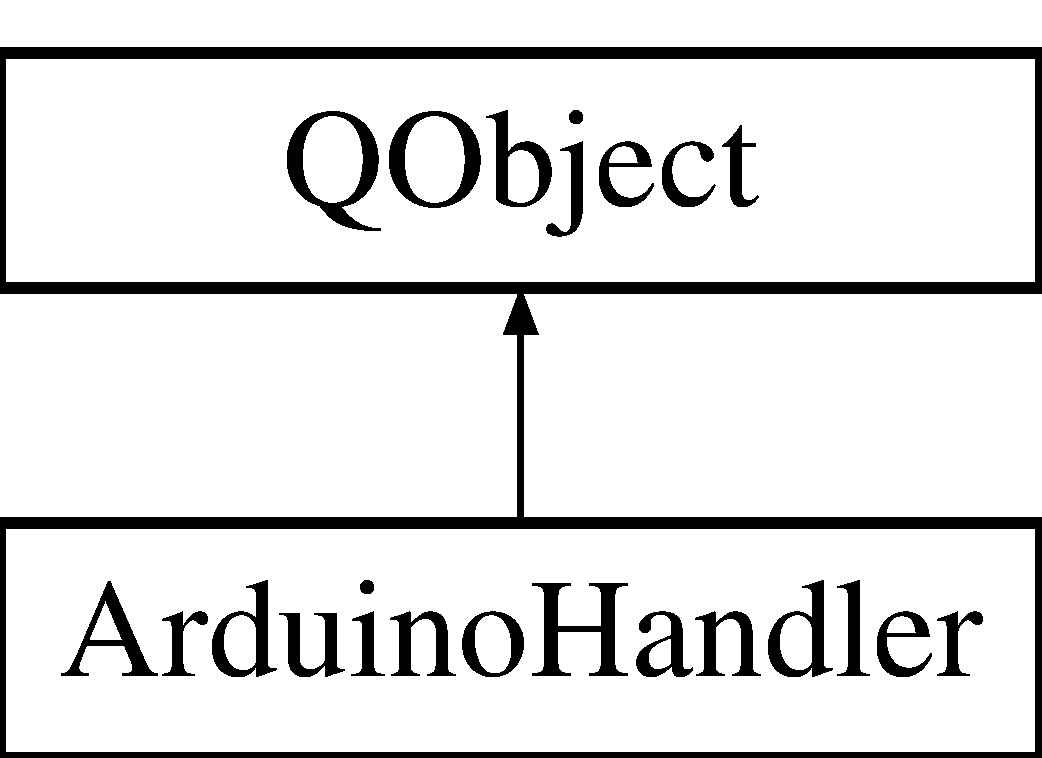
\includegraphics[height=2.000000cm]{class_arduino_handler}
\end{center}
\end{figure}
\subsection*{Signals}
\begin{DoxyCompactItemize}
\item 
\hypertarget{class_arduino_handler_a30502ceb7b61c7275c34061c604abd36}{}void \hyperlink{class_arduino_handler_a30502ceb7b61c7275c34061c604abd36}{left\+Pressed} ()\label{class_arduino_handler_a30502ceb7b61c7275c34061c604abd36}

\begin{DoxyCompactList}\small\item\em Emit lorsque l\textquotesingle{}Arduino Uno écrit \textquotesingle{}0\textquotesingle{} sur le port série. \end{DoxyCompactList}\item 
\hypertarget{class_arduino_handler_a07a1f4bd13691bd7c857c32c8112853b}{}void \hyperlink{class_arduino_handler_a07a1f4bd13691bd7c857c32c8112853b}{right\+Pressed} ()\label{class_arduino_handler_a07a1f4bd13691bd7c857c32c8112853b}

\begin{DoxyCompactList}\small\item\em Emit lorsque l\textquotesingle{}Arduino Uno écrit \textquotesingle{}1\textquotesingle{} sur le port série. \end{DoxyCompactList}\item 
\hypertarget{class_arduino_handler_a62ed3d1594cc371d54208225c2b2bdba}{}void \hyperlink{class_arduino_handler_a62ed3d1594cc371d54208225c2b2bdba}{up\+Pressed} ()\label{class_arduino_handler_a62ed3d1594cc371d54208225c2b2bdba}

\begin{DoxyCompactList}\small\item\em Emit lorsque l\textquotesingle{}Arduino Uno écrit \textquotesingle{}2\textquotesingle{} sur le port série. \end{DoxyCompactList}\item 
\hypertarget{class_arduino_handler_acba961acc6381ad00adf46bd0cf14ad0}{}void \hyperlink{class_arduino_handler_acba961acc6381ad00adf46bd0cf14ad0}{down\+Pressed} ()\label{class_arduino_handler_acba961acc6381ad00adf46bd0cf14ad0}

\begin{DoxyCompactList}\small\item\em Emit lorsque l\textquotesingle{}Arduino Uno écrit \textquotesingle{}3\textquotesingle{} sur le port série. \end{DoxyCompactList}\end{DoxyCompactItemize}
\subsection*{Public Member Functions}
\begin{DoxyCompactItemize}
\item 
\hyperlink{class_arduino_handler_add27f10e1b41f677d1810ddabc5e8870}{Arduino\+Handler} ()
\begin{DoxyCompactList}\small\item\em Constructeur de base \hyperlink{class_arduino_handler}{Arduino\+Handler}. \end{DoxyCompactList}\item 
void \hyperlink{class_arduino_handler_a15d8970b79dd96b1a0b0fdd118b0793f}{start} ()
\begin{DoxyCompactList}\small\item\em Connecte à l\textquotesingle{}Arduino Uno. \end{DoxyCompactList}\end{DoxyCompactItemize}
\subsection*{Protected Slots}
\begin{DoxyCompactItemize}
\item 
void \hyperlink{class_arduino_handler_a2b34ab08c171c918bc711c93810dadde}{mainloop} ()
\begin{DoxyCompactList}\small\item\em Boucle principale de lecture du port série. \end{DoxyCompactList}\end{DoxyCompactItemize}


\subsection{Detailed Description}
Classe gérant la connexion d\textquotesingle{}un Arduino Uno pour le contrôle du Pacman. 

\begin{DoxyAuthor}{Author}
Valentin D.\+d.\+G. 
\end{DoxyAuthor}
\begin{DoxyVersion}{Version}
1.\+0
\end{DoxyVersion}
Un \hyperlink{class_arduino_handler}{Arduino\+Handler} emet des signaux Gauche, Droite, Haut, Bas en fonction de la lecture (resp. \textquotesingle{}0\textquotesingle{}, \textquotesingle{}1\textquotesingle{}, \textquotesingle{}2\textquotesingle{} et \textquotesingle{}3\textquotesingle{}) sur le port série où est branché l\textquotesingle{}Arduino Uno. N\textquotesingle{}émet aucun signal si aucun Arduino n\textquotesingle{}est branché. Si plusieurs Arduinos sont branchés, l\textquotesingle{}\hyperlink{class_arduino_handler}{Arduino\+Handler} utilisera le premier disponible. 

\subsection{Constructor \& Destructor Documentation}
\hypertarget{class_arduino_handler_add27f10e1b41f677d1810ddabc5e8870}{}\index{Arduino\+Handler@{Arduino\+Handler}!Arduino\+Handler@{Arduino\+Handler}}
\index{Arduino\+Handler@{Arduino\+Handler}!Arduino\+Handler@{Arduino\+Handler}}
\subsubsection[{Arduino\+Handler()}]{\setlength{\rightskip}{0pt plus 5cm}Arduino\+Handler\+::\+Arduino\+Handler (
\begin{DoxyParamCaption}
{}
\end{DoxyParamCaption}
)}\label{class_arduino_handler_add27f10e1b41f677d1810ddabc5e8870}


Constructeur de base \hyperlink{class_arduino_handler}{Arduino\+Handler}. 

Initialise un \hyperlink{class_arduino_handler}{Arduino\+Handler}. Cependant, il faut démarrer manuellement la connexion via la méthode \hyperlink{class_arduino_handler_a15d8970b79dd96b1a0b0fdd118b0793f}{start()}. Le port série doit être ouvert avec un Baud rate de 9600. 

\subsection{Member Function Documentation}
\hypertarget{class_arduino_handler_a2b34ab08c171c918bc711c93810dadde}{}\index{Arduino\+Handler@{Arduino\+Handler}!mainloop@{mainloop}}
\index{mainloop@{mainloop}!Arduino\+Handler@{Arduino\+Handler}}
\subsubsection[{mainloop}]{\setlength{\rightskip}{0pt plus 5cm}void Arduino\+Handler\+::mainloop (
\begin{DoxyParamCaption}
{}
\end{DoxyParamCaption}
)\hspace{0.3cm}{\ttfamily [protected]}, {\ttfamily [slot]}}\label{class_arduino_handler_a2b34ab08c171c918bc711c93810dadde}


Boucle principale de lecture du port série. 

Emet left\+Pressed en lisant \textquotesingle{}0\textquotesingle{}. ~\newline
 Emet right\+Pressed en lisant \textquotesingle{}1\textquotesingle{}. ~\newline
 Emet up\+Pressed en lisant \textquotesingle{}2\textquotesingle{}. ~\newline
 Emet down\+Pressed en lisant \textquotesingle{}3\textquotesingle{}. \hypertarget{class_arduino_handler_a15d8970b79dd96b1a0b0fdd118b0793f}{}\index{Arduino\+Handler@{Arduino\+Handler}!start@{start}}
\index{start@{start}!Arduino\+Handler@{Arduino\+Handler}}
\subsubsection[{start()}]{\setlength{\rightskip}{0pt plus 5cm}void Arduino\+Handler\+::start (
\begin{DoxyParamCaption}
{}
\end{DoxyParamCaption}
)}\label{class_arduino_handler_a15d8970b79dd96b1a0b0fdd118b0793f}


Connecte à l\textquotesingle{}Arduino Uno. 

Connecte au port série du premier Arduino Uno trouvé. Si aucun Arduino Uno n\textquotesingle{}est disponible, cette fonction ne fait rien. La lecture du port est effectuée toutes les 20mscs. 

The documentation for this class was generated from the following files\+:\begin{DoxyCompactItemize}
\item 
arduinohandler.\+h\item 
arduinohandler.\+cpp\end{DoxyCompactItemize}

\hypertarget{class_double_position}{}\section{Double\+Position Class Reference}
\label{class_double_position}\index{Double\+Position@{Double\+Position}}


Classe imitant une position à virgule avec deux entiers.  




{\ttfamily \#include $<$doubleposition.\+h$>$}

\subsection*{Public Member Functions}
\begin{DoxyCompactItemize}
\item 
\hyperlink{class_double_position_a801bc7f47d6c1ada127b308e14538a3d}{Double\+Position} ()
\begin{DoxyCompactList}\small\item\em Constructeur de base \hyperlink{class_double_position}{Double\+Position}. \end{DoxyCompactList}\item 
\hyperlink{class_double_position_a496aec1866319f503156051b938eafbb}{Double\+Position} (Q\+Point int\+Pos, Q\+Point float\+Pos)
\begin{DoxyCompactList}\small\item\em Surcharge du constructeur de base. \end{DoxyCompactList}\item 
\hyperlink{class_double_position_a9eb14f4d74c0bc4dc9a30bcc765f93a4}{Double\+Position} (Q\+Dom\+Element elem)
\begin{DoxyCompactList}\small\item\em Surcharge du constructeur de base pour X\+M\+L. \end{DoxyCompactList}\item 
Q\+Point \hyperlink{class_double_position_afc3276b37b2cca9d982f4773b35a450a}{integer\+Position} () const 
\begin{DoxyCompactList}\small\item\em Getter (m\+\_\+integer\+Position). \end{DoxyCompactList}\item 
Q\+Point \hyperlink{class_double_position_aa5b3aff5c9c95efefb3f9625ec514fa0}{float\+Position} () const 
\begin{DoxyCompactList}\small\item\em Getter (m\+\_\+float\+Position). \end{DoxyCompactList}\item 
bool \hyperlink{class_double_position_a8531d86338f04961d875ee903adb9ec0}{is\+Float\+Position\+Null} () const 
\begin{DoxyCompactList}\small\item\em Analyse la partie réelle de la position. \end{DoxyCompactList}\item 
void \hyperlink{class_double_position_a9865b0c4bb41f8337d0063443d2edc7e}{increase\+X} (int pace)
\begin{DoxyCompactList}\small\item\em Augmente la coordonnée X réelle. \end{DoxyCompactList}\item 
void \hyperlink{class_double_position_a6b26f1e3875571911cecbcec20760193}{increase\+Y} (int pace)
\begin{DoxyCompactList}\small\item\em Augmente la coordonnée Y réelle. \end{DoxyCompactList}\item 
void \hyperlink{class_double_position_ab96be3ead7159a7e736bdf96f73cfbdc}{set\+Integer\+Position} (const Q\+Point \&\hyperlink{class_double_position_afc3276b37b2cca9d982f4773b35a450a}{integer\+Position})
\begin{DoxyCompactList}\small\item\em Setter (m\+\_\+integer\+Position). \end{DoxyCompactList}\item 
void \hyperlink{class_double_position_a0af7282f24900a3106ae324ca12c5def}{set\+Integer\+Position\+X} (int x)
\begin{DoxyCompactList}\small\item\em Setter (X de la partie entière) \end{DoxyCompactList}\item 
void \hyperlink{class_double_position_a513c186fb02d0b6549e7c80ece398a2b}{set\+Integer\+Position\+Y} (int y)
\begin{DoxyCompactList}\small\item\em Setter (Y de la partie entière) \end{DoxyCompactList}\item 
void \hyperlink{class_double_position_ae1730ae16bcc3365d2d3edfbaa66045c}{set\+Float\+Position} (const Q\+Point \&\hyperlink{class_double_position_aa5b3aff5c9c95efefb3f9625ec514fa0}{float\+Position})
\begin{DoxyCompactList}\small\item\em Setter (m\+\_\+float\+Position). \end{DoxyCompactList}\item 
void \hyperlink{class_double_position_a3b1a3c85dca66f2640556ffe47970ada}{set\+Float\+Position\+X} (int x)
\begin{DoxyCompactList}\small\item\em Setter (X de la partie réelle) \end{DoxyCompactList}\item 
void \hyperlink{class_double_position_a7f09cd0c1bda5695f6417f63b6a06798}{set\+Float\+Position\+Y} (int y)
\begin{DoxyCompactList}\small\item\em Setter (Y de la partie réelle) \end{DoxyCompactList}\item 
qreal \hyperlink{class_double_position_a5276d9c2b449a7e7c86545aea825cc75}{euclidian\+Distance\+To} (\hyperlink{class_double_position}{Double\+Position} const \&position)
\begin{DoxyCompactList}\small\item\em Calcule la distance euclidienne d\textquotesingle{}une position à l\textquotesingle{}autre. \end{DoxyCompactList}\end{DoxyCompactItemize}


\subsection{Detailed Description}
Classe imitant une position à virgule avec deux entiers. 

\begin{DoxyAuthor}{Author}
Valentin D.\+d.\+G. 
\end{DoxyAuthor}
\begin{DoxyVersion}{Version}
1.\+0
\end{DoxyVersion}
\hyperlink{class_double_position}{Double\+Position} utilise deux couples d\textquotesingle{}entiers afin de simuler un couple de réels afin d\textquotesingle{}éviter les pertes de précisions dûes à la représentation binaire. 

\subsection{Constructor \& Destructor Documentation}
\hypertarget{class_double_position_a801bc7f47d6c1ada127b308e14538a3d}{}\index{Double\+Position@{Double\+Position}!Double\+Position@{Double\+Position}}
\index{Double\+Position@{Double\+Position}!Double\+Position@{Double\+Position}}
\subsubsection[{Double\+Position()}]{\setlength{\rightskip}{0pt plus 5cm}Double\+Position\+::\+Double\+Position (
\begin{DoxyParamCaption}
{}
\end{DoxyParamCaption}
)}\label{class_double_position_a801bc7f47d6c1ada127b308e14538a3d}


Constructeur de base \hyperlink{class_double_position}{Double\+Position}. 

Constuit une \hyperlink{class_double_position}{Double\+Position} dont les valeurs sont nulles. \hypertarget{class_double_position_a496aec1866319f503156051b938eafbb}{}\index{Double\+Position@{Double\+Position}!Double\+Position@{Double\+Position}}
\index{Double\+Position@{Double\+Position}!Double\+Position@{Double\+Position}}
\subsubsection[{Double\+Position(\+Q\+Point int\+Pos, Q\+Point float\+Pos)}]{\setlength{\rightskip}{0pt plus 5cm}Double\+Position\+::\+Double\+Position (
\begin{DoxyParamCaption}
\item[{Q\+Point}]{int\+Pos, }
\item[{Q\+Point}]{float\+Pos}
\end{DoxyParamCaption}
)}\label{class_double_position_a496aec1866319f503156051b938eafbb}


Surcharge du constructeur de base. 


\begin{DoxyParams}[1]{Parameters}
\mbox{\tt in}  & {\em int\+Pos} & Partie entière de la position \\
\hline
\mbox{\tt in}  & {\em float\+Pos} & Partie réelle de la position\\
\hline
\end{DoxyParams}
Constuit une \hyperlink{class_double_position}{Double\+Position} dont les valeurs sont égales aux paramètres int\+Pos et float\+Pos donnés. \hypertarget{class_double_position_a9eb14f4d74c0bc4dc9a30bcc765f93a4}{}\index{Double\+Position@{Double\+Position}!Double\+Position@{Double\+Position}}
\index{Double\+Position@{Double\+Position}!Double\+Position@{Double\+Position}}
\subsubsection[{Double\+Position(\+Q\+Dom\+Element elem)}]{\setlength{\rightskip}{0pt plus 5cm}Double\+Position\+::\+Double\+Position (
\begin{DoxyParamCaption}
\item[{Q\+Dom\+Element}]{elem}
\end{DoxyParamCaption}
)}\label{class_double_position_a9eb14f4d74c0bc4dc9a30bcc765f93a4}


Surcharge du constructeur de base pour X\+M\+L. 


\begin{DoxyParams}[1]{Parameters}
\mbox{\tt in}  & {\em elem} & Balise X\+M\+L contenant les paramètres de la position\\
\hline
\end{DoxyParams}
Construit une \hyperlink{class_double_position}{Double\+Position} en fonction de l\textquotesingle{}élément X\+M\+L donné.
\begin{DoxyItemize}
\item ix \+: Coordonnée X entière.
\item iy \+: Coordonnée Y entière.
\item fx \+: Coordonnée X réelle. (half pour une demi-\/case, 0 pour les autres valeurs).
\item fy \+: Coordonnée Y réelle. (half pour une demi-\/case, 0 pour les autres valeurs). 
\end{DoxyItemize}

\subsection{Member Function Documentation}
\hypertarget{class_double_position_a5276d9c2b449a7e7c86545aea825cc75}{}\index{Double\+Position@{Double\+Position}!euclidian\+Distance\+To@{euclidian\+Distance\+To}}
\index{euclidian\+Distance\+To@{euclidian\+Distance\+To}!Double\+Position@{Double\+Position}}
\subsubsection[{euclidian\+Distance\+To(\+Double\+Position const \&position)}]{\setlength{\rightskip}{0pt plus 5cm}qreal Double\+Position\+::euclidian\+Distance\+To (
\begin{DoxyParamCaption}
\item[{{\bf Double\+Position} const \&}]{position}
\end{DoxyParamCaption}
)}\label{class_double_position_a5276d9c2b449a7e7c86545aea825cc75}


Calcule la distance euclidienne d\textquotesingle{}une position à l\textquotesingle{}autre. 


\begin{DoxyParams}{Parameters}
{\em position} & Position à partir de laquelle calculer la distance. \\
\hline
\end{DoxyParams}
\begin{DoxyReturn}{Returns}
Distance euclidienne entre les deux positions (en double).
\end{DoxyReturn}
((ix1.\+fx1 -\/ ix2.\+fx2)$^\wedge$2 + (iy1.\+fy1 -\/ iy2.\+fy2)$^\wedge$2)$^\wedge$(1/2) \hypertarget{class_double_position_aa5b3aff5c9c95efefb3f9625ec514fa0}{}\index{Double\+Position@{Double\+Position}!float\+Position@{float\+Position}}
\index{float\+Position@{float\+Position}!Double\+Position@{Double\+Position}}
\subsubsection[{float\+Position() const }]{\setlength{\rightskip}{0pt plus 5cm}Q\+Point Double\+Position\+::float\+Position (
\begin{DoxyParamCaption}
{}
\end{DoxyParamCaption}
) const}\label{class_double_position_aa5b3aff5c9c95efefb3f9625ec514fa0}


Getter (m\+\_\+float\+Position). 

\begin{DoxyReturn}{Returns}
Partie réelle de la position. 
\end{DoxyReturn}
\hypertarget{class_double_position_a9865b0c4bb41f8337d0063443d2edc7e}{}\index{Double\+Position@{Double\+Position}!increase\+X@{increase\+X}}
\index{increase\+X@{increase\+X}!Double\+Position@{Double\+Position}}
\subsubsection[{increase\+X(int pace)}]{\setlength{\rightskip}{0pt plus 5cm}void Double\+Position\+::increase\+X (
\begin{DoxyParamCaption}
\item[{int}]{pace}
\end{DoxyParamCaption}
)}\label{class_double_position_a9865b0c4bb41f8337d0063443d2edc7e}


Augmente la coordonnée X réelle. 


\begin{DoxyParams}[1]{Parameters}
\mbox{\tt in}  & {\em pace} & Pas d\textquotesingle{}augmentation de la partie réelle (en X).\\
\hline
\end{DoxyParams}
Augmente de pace la partie réelle selon X. ~\newline
 Si la partie réelle excède M\+A\+X\+\_\+\+F\+L\+O\+A\+T\+\_\+\+P\+O\+S alors elle devient nulle et la partie entière est augmentée de 1. ~\newline
 De même, si la partie réelle devient inférieure à 0, la partie entière diminue de 1 et la partie réelle est mise à M\+A\+X\+\_\+\+F\+L\+O\+A\+T\+\_\+\+P\+O\+S moins le pas. ~\newline
 Si la partie réelle s\textquotesingle{}approche de 0, elle devient alors nulle. \hypertarget{class_double_position_a6b26f1e3875571911cecbcec20760193}{}\index{Double\+Position@{Double\+Position}!increase\+Y@{increase\+Y}}
\index{increase\+Y@{increase\+Y}!Double\+Position@{Double\+Position}}
\subsubsection[{increase\+Y(int pace)}]{\setlength{\rightskip}{0pt plus 5cm}void Double\+Position\+::increase\+Y (
\begin{DoxyParamCaption}
\item[{int}]{pace}
\end{DoxyParamCaption}
)}\label{class_double_position_a6b26f1e3875571911cecbcec20760193}


Augmente la coordonnée Y réelle. 


\begin{DoxyParams}[1]{Parameters}
\mbox{\tt in}  & {\em pace} & Pas d\textquotesingle{}augmentation de la partie réelle (en Y).\\
\hline
\end{DoxyParams}
Augmente de pace la partie réelle selon Y. ~\newline
 Si la partie réelle excède M\+A\+X\+\_\+\+F\+L\+O\+A\+T\+\_\+\+P\+O\+S alors elle devient nulle et la partie entière est augmentée de 1. ~\newline
 De même, si la partie réelle devient inférieure à 0, la partie entière diminue de 1 et la partie réelle est mise à M\+A\+X\+\_\+\+F\+L\+O\+A\+T\+\_\+\+P\+O\+S moins le pas. ~\newline
 Si la partie réelle s\textquotesingle{}approche de 0, elle devient alors nulle. \hypertarget{class_double_position_afc3276b37b2cca9d982f4773b35a450a}{}\index{Double\+Position@{Double\+Position}!integer\+Position@{integer\+Position}}
\index{integer\+Position@{integer\+Position}!Double\+Position@{Double\+Position}}
\subsubsection[{integer\+Position() const }]{\setlength{\rightskip}{0pt plus 5cm}Q\+Point Double\+Position\+::integer\+Position (
\begin{DoxyParamCaption}
{}
\end{DoxyParamCaption}
) const}\label{class_double_position_afc3276b37b2cca9d982f4773b35a450a}


Getter (m\+\_\+integer\+Position). 

\begin{DoxyReturn}{Returns}
Partie entière de la position. 
\end{DoxyReturn}
\hypertarget{class_double_position_a8531d86338f04961d875ee903adb9ec0}{}\index{Double\+Position@{Double\+Position}!is\+Float\+Position\+Null@{is\+Float\+Position\+Null}}
\index{is\+Float\+Position\+Null@{is\+Float\+Position\+Null}!Double\+Position@{Double\+Position}}
\subsubsection[{is\+Float\+Position\+Null() const }]{\setlength{\rightskip}{0pt plus 5cm}bool Double\+Position\+::is\+Float\+Position\+Null (
\begin{DoxyParamCaption}
{}
\end{DoxyParamCaption}
) const}\label{class_double_position_a8531d86338f04961d875ee903adb9ec0}


Analyse la partie réelle de la position. 

\begin{DoxyReturn}{Returns}
true si la partie réelle est nulle, sinon false. 
\end{DoxyReturn}
\hypertarget{class_double_position_ae1730ae16bcc3365d2d3edfbaa66045c}{}\index{Double\+Position@{Double\+Position}!set\+Float\+Position@{set\+Float\+Position}}
\index{set\+Float\+Position@{set\+Float\+Position}!Double\+Position@{Double\+Position}}
\subsubsection[{set\+Float\+Position(const Q\+Point \&float\+Position)}]{\setlength{\rightskip}{0pt plus 5cm}void Double\+Position\+::set\+Float\+Position (
\begin{DoxyParamCaption}
\item[{const Q\+Point \&}]{float\+Position}
\end{DoxyParamCaption}
)}\label{class_double_position_ae1730ae16bcc3365d2d3edfbaa66045c}


Setter (m\+\_\+float\+Position). 


\begin{DoxyParams}{Parameters}
{\em float\+Position} & Nouvelle position (après la virgule) \\
\hline
\end{DoxyParams}
\hypertarget{class_double_position_a3b1a3c85dca66f2640556ffe47970ada}{}\index{Double\+Position@{Double\+Position}!set\+Float\+Position\+X@{set\+Float\+Position\+X}}
\index{set\+Float\+Position\+X@{set\+Float\+Position\+X}!Double\+Position@{Double\+Position}}
\subsubsection[{set\+Float\+Position\+X(int x)}]{\setlength{\rightskip}{0pt plus 5cm}void Double\+Position\+::set\+Float\+Position\+X (
\begin{DoxyParamCaption}
\item[{int}]{x}
\end{DoxyParamCaption}
)}\label{class_double_position_a3b1a3c85dca66f2640556ffe47970ada}


Setter (X de la partie réelle) 


\begin{DoxyParams}{Parameters}
{\em x} & Nouveau X de la partière réelle \\
\hline
\end{DoxyParams}
\hypertarget{class_double_position_a7f09cd0c1bda5695f6417f63b6a06798}{}\index{Double\+Position@{Double\+Position}!set\+Float\+Position\+Y@{set\+Float\+Position\+Y}}
\index{set\+Float\+Position\+Y@{set\+Float\+Position\+Y}!Double\+Position@{Double\+Position}}
\subsubsection[{set\+Float\+Position\+Y(int y)}]{\setlength{\rightskip}{0pt plus 5cm}void Double\+Position\+::set\+Float\+Position\+Y (
\begin{DoxyParamCaption}
\item[{int}]{y}
\end{DoxyParamCaption}
)}\label{class_double_position_a7f09cd0c1bda5695f6417f63b6a06798}


Setter (Y de la partie réelle) 


\begin{DoxyParams}{Parameters}
{\em y} & Nouveau Y de la partière réelle \\
\hline
\end{DoxyParams}
\begin{DoxyReturn}{Returns}

\end{DoxyReturn}
\hypertarget{class_double_position_ab96be3ead7159a7e736bdf96f73cfbdc}{}\index{Double\+Position@{Double\+Position}!set\+Integer\+Position@{set\+Integer\+Position}}
\index{set\+Integer\+Position@{set\+Integer\+Position}!Double\+Position@{Double\+Position}}
\subsubsection[{set\+Integer\+Position(const Q\+Point \&integer\+Position)}]{\setlength{\rightskip}{0pt plus 5cm}void Double\+Position\+::set\+Integer\+Position (
\begin{DoxyParamCaption}
\item[{const Q\+Point \&}]{integer\+Position}
\end{DoxyParamCaption}
)}\label{class_double_position_ab96be3ead7159a7e736bdf96f73cfbdc}


Setter (m\+\_\+integer\+Position). 


\begin{DoxyParams}{Parameters}
{\em integer\+Position} & Nouvelle position entière \\
\hline
\end{DoxyParams}
\hypertarget{class_double_position_a0af7282f24900a3106ae324ca12c5def}{}\index{Double\+Position@{Double\+Position}!set\+Integer\+Position\+X@{set\+Integer\+Position\+X}}
\index{set\+Integer\+Position\+X@{set\+Integer\+Position\+X}!Double\+Position@{Double\+Position}}
\subsubsection[{set\+Integer\+Position\+X(int x)}]{\setlength{\rightskip}{0pt plus 5cm}void Double\+Position\+::set\+Integer\+Position\+X (
\begin{DoxyParamCaption}
\item[{int}]{x}
\end{DoxyParamCaption}
)}\label{class_double_position_a0af7282f24900a3106ae324ca12c5def}


Setter (X de la partie entière) 


\begin{DoxyParams}{Parameters}
{\em x} & Nouveau X de la partière entière \\
\hline
\end{DoxyParams}
\hypertarget{class_double_position_a513c186fb02d0b6549e7c80ece398a2b}{}\index{Double\+Position@{Double\+Position}!set\+Integer\+Position\+Y@{set\+Integer\+Position\+Y}}
\index{set\+Integer\+Position\+Y@{set\+Integer\+Position\+Y}!Double\+Position@{Double\+Position}}
\subsubsection[{set\+Integer\+Position\+Y(int y)}]{\setlength{\rightskip}{0pt plus 5cm}void Double\+Position\+::set\+Integer\+Position\+Y (
\begin{DoxyParamCaption}
\item[{int}]{y}
\end{DoxyParamCaption}
)}\label{class_double_position_a513c186fb02d0b6549e7c80ece398a2b}


Setter (Y de la partie entière) 


\begin{DoxyParams}{Parameters}
{\em y} & Nouveau Y de la partière entière \\
\hline
\end{DoxyParams}


The documentation for this class was generated from the following files\+:\begin{DoxyCompactItemize}
\item 
doubleposition.\+h\item 
doubleposition.\+cpp\end{DoxyCompactItemize}

\hypertarget{class_firework}{}\section{Firework Class Reference}
\label{class_firework}\index{Firework@{Firework}}


Classe d\textquotesingle{}animation de feu d\textquotesingle{}artifices.  




{\ttfamily \#include $<$firework.\+h$>$}

\subsection*{Public Member Functions}
\begin{DoxyCompactItemize}
\item 
\hyperlink{class_firework_af032da470d5bca6f9a36bec0a3228b8a}{Firework} (int width, int height)
\begin{DoxyCompactList}\small\item\em Constructeur de base de la classe \hyperlink{class_firework}{Firework}. \end{DoxyCompactList}\item 
\hypertarget{class_firework_aba631b83c2df26f8bd9fa124bd711974}{}void \hyperlink{class_firework_aba631b83c2df26f8bd9fa124bd711974}{init} ()\label{class_firework_aba631b83c2df26f8bd9fa124bd711974}

\begin{DoxyCompactList}\small\item\em Réinitialise les paramètres aléatoires de l\textquotesingle{}objet. \end{DoxyCompactList}\item 
Q\+Pixmap \hyperlink{class_firework_a23dd6268486eb91b6c5cfa2279bc0b41}{paint\+Firework} ()
\begin{DoxyCompactList}\small\item\em Calcule et renvoie la prochaine image de l\textquotesingle{}animation. \end{DoxyCompactList}\item 
Q\+Point \hyperlink{class_firework_ace6e4734843019521c0e2a244e5f6c1c}{center} () const 
\begin{DoxyCompactList}\small\item\em Getter. \end{DoxyCompactList}\end{DoxyCompactItemize}


\subsection{Detailed Description}
Classe d\textquotesingle{}animation de feu d\textquotesingle{}artifices. 

\begin{DoxyAuthor}{Author}
Valentin D.\+d.\+G. 
\end{DoxyAuthor}
\begin{DoxyVersion}{Version}
1.\+0
\end{DoxyVersion}
Cette classe s\textquotesingle{}instancie avec la taille maximale de la destination (par exemple, la taille de l\textquotesingle{}écran) et génère automatiquement une image. L\textquotesingle{}image générée ne prend pas en compte la position de l\textquotesingle{}objet (afin de placer cette image librement) et fait la taille maximale que fera l\textquotesingle{}animation. L\textquotesingle{}image générée est modifiée à chaque fois que la fonction est appelée afin de calculer la prochaine image de l\textquotesingle{}animation.

L\textquotesingle{}animation en elle même affiche une dispersion de lignes qui simulent un feu d\textquotesingle{}artifice. Les lignes peuvent prendre plusieurs couleurs aléatoires et s\textquotesingle{}estompent au fil du temps. La façon dont les lignes s\textquotesingle{}estompent simule un effet de deccélaration soudaine (comme dans le cas d\textquotesingle{}une explosion). 

\subsection{Constructor \& Destructor Documentation}
\hypertarget{class_firework_af032da470d5bca6f9a36bec0a3228b8a}{}\index{Firework@{Firework}!Firework@{Firework}}
\index{Firework@{Firework}!Firework@{Firework}}
\subsubsection[{Firework(int width, int height)}]{\setlength{\rightskip}{0pt plus 5cm}Firework\+::\+Firework (
\begin{DoxyParamCaption}
\item[{int}]{width, }
\item[{int}]{height}
\end{DoxyParamCaption}
)}\label{class_firework_af032da470d5bca6f9a36bec0a3228b8a}


Constructeur de base de la classe \hyperlink{class_firework}{Firework}. 


\begin{DoxyParams}{Parameters}
{\em width} & Largeur de la destination qui affichera l\textquotesingle{}animation. \\
\hline
{\em height} & Hauteur de la destination qui affichera l\textquotesingle{}animation.\\
\hline
\end{DoxyParams}
Lors de la construction de l\textquotesingle{}objet, les différents paramètres aléatoire de la classe (tels que la taille de l\textquotesingle{}animation, les lignes qui la compose, leur longueur) sont automatiquement réglés (à une valeur aléatoire). Cependant, la classe ne modifie pas la graine aléatore utilisée. Afin de réinitialiser les paramètres de façon aléatoire, voire la fonction \hyperlink{class_firework_aba631b83c2df26f8bd9fa124bd711974}{init()}; 

\subsection{Member Function Documentation}
\hypertarget{class_firework_ace6e4734843019521c0e2a244e5f6c1c}{}\index{Firework@{Firework}!center@{center}}
\index{center@{center}!Firework@{Firework}}
\subsubsection[{center() const }]{\setlength{\rightskip}{0pt plus 5cm}Q\+Point Firework\+::center (
\begin{DoxyParamCaption}
{}
\end{DoxyParamCaption}
) const}\label{class_firework_ace6e4734843019521c0e2a244e5f6c1c}


Getter. 

\begin{DoxyReturn}{Returns}
Centre de l\textquotesingle{}animation.
\end{DoxyReturn}
Généré aléatoirement au sein de la taille donnée lors de la construction de l\textquotesingle{}objet. \hypertarget{class_firework_a23dd6268486eb91b6c5cfa2279bc0b41}{}\index{Firework@{Firework}!paint\+Firework@{paint\+Firework}}
\index{paint\+Firework@{paint\+Firework}!Firework@{Firework}}
\subsubsection[{paint\+Firework()}]{\setlength{\rightskip}{0pt plus 5cm}Q\+Pixmap Firework\+::paint\+Firework (
\begin{DoxyParamCaption}
{}
\end{DoxyParamCaption}
)}\label{class_firework_a23dd6268486eb91b6c5cfa2279bc0b41}


Calcule et renvoie la prochaine image de l\textquotesingle{}animation. 

\begin{DoxyReturn}{Returns}
Une frame de l\textquotesingle{}animation (dans l\textquotesingle{}ordre). 
\end{DoxyReturn}


The documentation for this class was generated from the following files\+:\begin{DoxyCompactItemize}
\item 
firework.\+h\item 
firework.\+cpp\end{DoxyCompactItemize}

\hypertarget{class_game}{}\section{Game Class Reference}
\label{class_game}\index{Game@{Game}}


La classe \hyperlink{class_game}{Game} gère l\textquotesingle{}ensemble des paramètres de Pacman.  




{\ttfamily \#include $<$game.\+h$>$}

Inheritance diagram for Game\+:\begin{figure}[H]
\begin{center}
\leavevmode
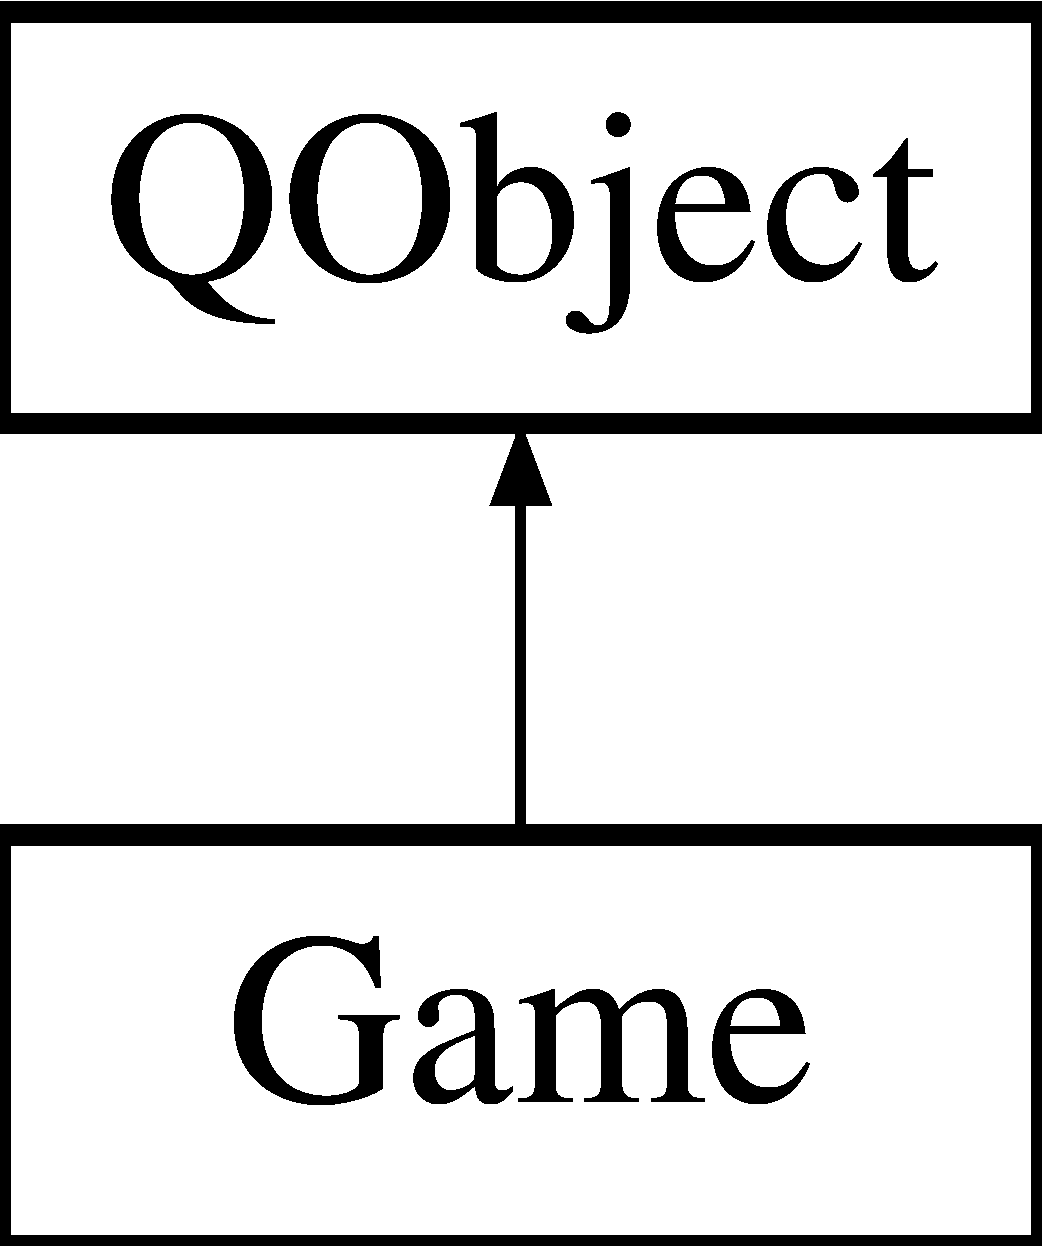
\includegraphics[height=2.000000cm]{class_game}
\end{center}
\end{figure}
\subsection*{Public Slots}
\begin{DoxyCompactItemize}
\item 
\hypertarget{class_game_a3c0e737b028fae5e5fc323efe6326880}{}void \hyperlink{class_game_a3c0e737b028fae5e5fc323efe6326880}{next\+Game\+Frame} ()\label{class_game_a3c0e737b028fae5e5fc323efe6326880}

\begin{DoxyCompactList}\small\item\em Calcule la prochaine frame. \end{DoxyCompactList}\item 
\hypertarget{class_game_a5ec2daf2a7fe95ee03dea84b4f5d6883}{}void \hyperlink{class_game_a5ec2daf2a7fe95ee03dea84b4f5d6883}{resume\+Game} ()\label{class_game_a5ec2daf2a7fe95ee03dea84b4f5d6883}

\begin{DoxyCompactList}\small\item\em Relance le timer du jeu. \end{DoxyCompactList}\end{DoxyCompactItemize}
\subsection*{Public Member Functions}
\begin{DoxyCompactItemize}
\item 
\hyperlink{class_game_a07651e12402cbf4ffb116870594cb347}{Game} (Q\+Dom\+Document $\ast$dom)
\begin{DoxyCompactList}\small\item\em Constructeur de base de la classe \hyperlink{class_game}{Game}. \end{DoxyCompactList}\item 
void \hyperlink{class_game_ae8638ccdb0ef3bf39a6affa30aa1258f}{start\+Game} ()
\begin{DoxyCompactList}\small\item\em Démarre le jeu avec F\+P\+S (cf. \hyperlink{pacmanparameters_8h_source}{pacmanparameters.\+h}) images par seconde. \end{DoxyCompactList}\item 
int \hyperlink{class_game_aa23771d9b5897ab65aae22f930b6e7a8}{current\+Level} () const 
\begin{DoxyCompactList}\small\item\em Getter. \end{DoxyCompactList}\item 
void \hyperlink{class_game_ad7c1d10b807c0707e4b9f71e975135f4}{set\+Current\+Level} (int \hyperlink{class_game_aa23771d9b5897ab65aae22f930b6e7a8}{current\+Level})
\begin{DoxyCompactList}\small\item\em Setter. \end{DoxyCompactList}\item 
Q\+List$<$ \hyperlink{class_level}{Level} $\ast$ $>$ \hyperlink{class_game_a827328224e2d00cca5534a87b655e3c4}{levels} () const 
\begin{DoxyCompactList}\small\item\em Getter. \end{DoxyCompactList}\item 
int \hyperlink{class_game_acd638924aa59358846e55e78d272a2ec}{score} () const 
\begin{DoxyCompactList}\small\item\em Getter. \end{DoxyCompactList}\item 
int \hyperlink{class_game_a5cf4da142ff72734ee8713b2c37b2b9b}{lifes} () const 
\begin{DoxyCompactList}\small\item\em Getter. \end{DoxyCompactList}\item 
Q\+Timer $\ast$ \hyperlink{class_game_a8c93ee78acb3dc311aaf5b7bae06e70c}{timer} () const 
\begin{DoxyCompactList}\small\item\em Getter. \end{DoxyCompactList}\item 
Q\+Image \hyperlink{class_game_a355b625103201150c07114b4b2fccb03}{image} () const 
\begin{DoxyCompactList}\small\item\em Getter. \end{DoxyCompactList}\item 
void \hyperlink{class_game_aa9db7117b627f79bac876506fa6733d3}{set\+Pacman\+Direction} (int direction)
\begin{DoxyCompactList}\small\item\em Modifie la direction actuelle du joueur. \end{DoxyCompactList}\end{DoxyCompactItemize}
\subsection*{Protected Slots}
\begin{DoxyCompactItemize}
\item 
\hypertarget{class_game_afaad4867b30abbd7005f336c9f270986}{}void \hyperlink{class_game_afaad4867b30abbd7005f336c9f270986}{on\+Pellet\+Eaten} ()\label{class_game_afaad4867b30abbd7005f336c9f270986}

\begin{DoxyCompactList}\small\item\em Modifie les valeurs du jeu lorsque le joueur mange une pastille. \end{DoxyCompactList}\item 
\hypertarget{class_game_ad3a2fed489f6bb930e3a88785ddf8c9d}{}void \hyperlink{class_game_ad3a2fed489f6bb930e3a88785ddf8c9d}{on\+Energizer\+Eaten} ()\label{class_game_ad3a2fed489f6bb930e3a88785ddf8c9d}

\begin{DoxyCompactList}\small\item\em Modifie les valeurs du jeu lorsque le joueur mange un énergisant et fait peur aux fantômes. \end{DoxyCompactList}\end{DoxyCompactItemize}


\subsection{Detailed Description}
La classe \hyperlink{class_game}{Game} gère l\textquotesingle{}ensemble des paramètres de Pacman. 

\begin{DoxyAuthor}{Author}
Valentin D.\+d.\+G. 
\end{DoxyAuthor}
\begin{DoxyVersion}{Version}
1.\+0
\end{DoxyVersion}
La classe \hyperlink{class_game}{Game} s\textquotesingle{}occupe de gérer l\textquotesingle{}ensemble des niveaux, en leur faisant calculer les déplacements des unités. La classe \hyperlink{class_game}{Game} s\textquotesingle{}occupe aussi de tous les éléments qui sont communs à tous les niveaux (tels que le score ou le nombre de vies du Pacman). Enfin, la classe \hyperlink{class_game}{Game} effectue le rendu final de la grille (sans les à côtés commme l\textquotesingle{}affichage du score) qu\textquotesingle{}il fait calculer au niveau actuellement en cours.

N\+O\+T\+E \+:
\begin{DoxyItemize}
\item La classe \hyperlink{class_game}{Game} ne gère pas encore le passage d\textquotesingle{}un niveau à l\textquotesingle{}autre.
\item La classe \hyperlink{class_game}{Game} ne gère pas encore le son.
\item La classe \hyperlink{class_game}{Game} ne dispose pas encore de toutes les animations.
\item La classe \hyperlink{class_game}{Game} ne dispose pas encore de la table de correspondance des textures. 
\end{DoxyItemize}

\subsection{Constructor \& Destructor Documentation}
\hypertarget{class_game_a07651e12402cbf4ffb116870594cb347}{}\index{Game@{Game}!Game@{Game}}
\index{Game@{Game}!Game@{Game}}
\subsubsection[{Game(\+Q\+Dom\+Document $\ast$dom)}]{\setlength{\rightskip}{0pt plus 5cm}Game\+::\+Game (
\begin{DoxyParamCaption}
\item[{Q\+Dom\+Document $\ast$}]{dom}
\end{DoxyParamCaption}
)}\label{class_game_a07651e12402cbf4ffb116870594cb347}


Constructeur de base de la classe \hyperlink{class_game}{Game}. 


\begin{DoxyParams}{Parameters}
{\em dom} & Document X\+M\+L d\textquotesingle{}où le jeu charge toutes les données.\\
\hline
\end{DoxyParams}
Exemple (3x3 avec 5 textures)\+:
\begin{DoxyItemize}
\item $<$?xml version=\char`\"{}1.\+0\char`\"{} encoding=\char`\"{}\+I\+S\+O-\/8859-\/1\char`\"{}?$>$
\item $<$root$>$
\begin{DoxyItemize}
\item $<$\hyperlink{class_level}{Level}$>$
\begin{DoxyItemize}
\item $<$\hyperlink{class_grid}{Grid}$>$
\begin{DoxyItemize}
\item $<$Tile\+Count height=\char`\"{}3\char`\"{} width=\char`\"{}3\char`\"{}/$>$
\item $<$Tile\+Size height=\char`\"{}24\char`\"{} width=\char`\"{}24\char`\"{}/$>$
\item $<$Grid\+Values values=\char`\"{}aaacdebbb\char`\"{}/$>$
\item $<$Texture filename=\char`\"{}\+Texture1.\+png\char`\"{}/$>$
\item $<$Texture filename=\char`\"{}\+Texture2.\+png\char`\"{}/$>$
\item $<$Texture filename=\char`\"{}\+Texture\+\_\+\+Pastille.\+png\char`\"{}/$>$
\item $<$Texture filename=\char`\"{}\+Texture\+\_\+\+Energisant.\+png\char`\"{}/$>$
\item $<$Texture filename=\char`\"{}\+Texture\+\_\+\+Vide.\+png\char`\"{}/$>$
\item $<$Collisions\+Grid values=\char`\"{}000111000\char`\"{}/$>$
\item $<$Ghost\+House x=\char`\"{}1\char`\"{} y=\char`\"{}1\char`\"{} width=\char`\"{}1\char`\"{} height=\char`\"{}1\char`\"{}/$>$
\end{DoxyItemize}
\item $<$/ \hyperlink{class_grid}{Grid}$>$
\item $<$Player ix=\char`\"{}0\char`\"{} iy=\char`\"{}0\char`\"{} speed=\char`\"{}77\char`\"{} sspeed = \char`\"{}91\char`\"{} fx = \char`\"{}half\char`\"{}/$>$
\item $<$Blinky ix=\char`\"{}1\char`\"{} iy=\char`\"{}2\char`\"{} speed=\char`\"{}71\char`\"{} sspeed = \char`\"{}50\char`\"{} cornerx=\char`\"{}26\char`\"{} cornery=\char`\"{}-\/2\char`\"{} fx = \char`\"{}half\char`\"{}/$>$
\item $<$Pinky ix=\char`\"{}2\char`\"{} iy=\char`\"{}2\char`\"{} speed=\char`\"{}71\char`\"{} sspeed = \char`\"{}50\char`\"{} cornerx=\char`\"{}2\char`\"{} cornery=\char`\"{}-\/2\char`\"{}/$>$
\item $<$Inky ix=\char`\"{}1\char`\"{} iy=\char`\"{}2\char`\"{} speed=\char`\"{}71\char`\"{} sspeed = \char`\"{}50\char`\"{} cornerx=\char`\"{}28\char`\"{} cornery=\char`\"{}32\char`\"{} fx = \char`\"{}half\char`\"{}/$>$
\item $<$Clyde ix=\char`\"{}2\char`\"{} iy=\char`\"{}2\char`\"{} speed=\char`\"{}71\char`\"{} sspeed = \char`\"{}50\char`\"{} cornerx=\char`\"{}0\char`\"{} cornery=\char`\"{}32\char`\"{}/$>$
\item $<$\hyperlink{class_ghost_timer}{Ghost\+Timer}$>$
\begin{DoxyItemize}
\item $<$Step time=\char`\"{}7\char`\"{} mode=\char`\"{}0\char`\"{}/$>$
\item $<$Step time=\char`\"{}20\char`\"{} mode=\char`\"{}1\char`\"{}/$>$
\item $<$Step time=\char`\"{}7\char`\"{} mode=\char`\"{}0\char`\"{}/$>$
\end{DoxyItemize}
\item $<$/ \hyperlink{class_ghost_timer}{Ghost\+Timer}$>$
\item $<$Scared\+Mode duration=\char`\"{}6000\char`\"{} flashs=\char`\"{}5\char`\"{}/$>$
\end{DoxyItemize}
\item $<$/ \hyperlink{class_level}{Level}$>$
\end{DoxyItemize}
\item $<$/root$>$ 
\end{DoxyItemize}

\subsection{Member Function Documentation}
\hypertarget{class_game_aa23771d9b5897ab65aae22f930b6e7a8}{}\index{Game@{Game}!current\+Level@{current\+Level}}
\index{current\+Level@{current\+Level}!Game@{Game}}
\subsubsection[{current\+Level() const }]{\setlength{\rightskip}{0pt plus 5cm}int Game\+::current\+Level (
\begin{DoxyParamCaption}
{}
\end{DoxyParamCaption}
) const}\label{class_game_aa23771d9b5897ab65aae22f930b6e7a8}


Getter. 

\begin{DoxyReturn}{Returns}
Niveau actuellement utilisé par le Jeu. 
\end{DoxyReturn}
\hypertarget{class_game_a355b625103201150c07114b4b2fccb03}{}\index{Game@{Game}!image@{image}}
\index{image@{image}!Game@{Game}}
\subsubsection[{image() const }]{\setlength{\rightskip}{0pt plus 5cm}Q\+Image Game\+::image (
\begin{DoxyParamCaption}
{}
\end{DoxyParamCaption}
) const}\label{class_game_a355b625103201150c07114b4b2fccb03}


Getter. 

\begin{DoxyReturn}{Returns}
Grille du jeu sous forme d\textquotesingle{}image. 
\end{DoxyReturn}
\hypertarget{class_game_a827328224e2d00cca5534a87b655e3c4}{}\index{Game@{Game}!levels@{levels}}
\index{levels@{levels}!Game@{Game}}
\subsubsection[{levels() const }]{\setlength{\rightskip}{0pt plus 5cm}Q\+List$<$ {\bf Level} $\ast$ $>$ Game\+::levels (
\begin{DoxyParamCaption}
{}
\end{DoxyParamCaption}
) const}\label{class_game_a827328224e2d00cca5534a87b655e3c4}


Getter. 

\begin{DoxyReturn}{Returns}
La liste de tous les niveaux du jeu. 
\end{DoxyReturn}
\hypertarget{class_game_a5cf4da142ff72734ee8713b2c37b2b9b}{}\index{Game@{Game}!lifes@{lifes}}
\index{lifes@{lifes}!Game@{Game}}
\subsubsection[{lifes() const }]{\setlength{\rightskip}{0pt plus 5cm}int Game\+::lifes (
\begin{DoxyParamCaption}
{}
\end{DoxyParamCaption}
) const}\label{class_game_a5cf4da142ff72734ee8713b2c37b2b9b}


Getter. 

\begin{DoxyReturn}{Returns}
Nombre de vies du joueur. 
\end{DoxyReturn}
\hypertarget{class_game_acd638924aa59358846e55e78d272a2ec}{}\index{Game@{Game}!score@{score}}
\index{score@{score}!Game@{Game}}
\subsubsection[{score() const }]{\setlength{\rightskip}{0pt plus 5cm}int Game\+::score (
\begin{DoxyParamCaption}
{}
\end{DoxyParamCaption}
) const}\label{class_game_acd638924aa59358846e55e78d272a2ec}


Getter. 

\begin{DoxyReturn}{Returns}
Score actuel du joueur. 
\end{DoxyReturn}
\hypertarget{class_game_ad7c1d10b807c0707e4b9f71e975135f4}{}\index{Game@{Game}!set\+Current\+Level@{set\+Current\+Level}}
\index{set\+Current\+Level@{set\+Current\+Level}!Game@{Game}}
\subsubsection[{set\+Current\+Level(int current\+Level)}]{\setlength{\rightskip}{0pt plus 5cm}void Game\+::set\+Current\+Level (
\begin{DoxyParamCaption}
\item[{int}]{current\+Level}
\end{DoxyParamCaption}
)}\label{class_game_ad7c1d10b807c0707e4b9f71e975135f4}


Setter. 


\begin{DoxyParams}{Parameters}
{\em current\+Level} & Change le niveau utilisé par le Jeu. \\
\hline
\end{DoxyParams}
\hypertarget{class_game_aa9db7117b627f79bac876506fa6733d3}{}\index{Game@{Game}!set\+Pacman\+Direction@{set\+Pacman\+Direction}}
\index{set\+Pacman\+Direction@{set\+Pacman\+Direction}!Game@{Game}}
\subsubsection[{set\+Pacman\+Direction(int direction)}]{\setlength{\rightskip}{0pt plus 5cm}void Game\+::set\+Pacman\+Direction (
\begin{DoxyParamCaption}
\item[{int}]{direction}
\end{DoxyParamCaption}
)}\label{class_game_aa9db7117b627f79bac876506fa6733d3}


Modifie la direction actuelle du joueur. 


\begin{DoxyParams}{Parameters}
{\em direction} & Nouvelle direction\\
\hline
\end{DoxyParams}
Essaie de modifier la direction actuelle du joueur par le paramètre. Si le joueur ne peut pas effectuer ce mouvement immédiatement, la direction est stockée et sera prise dès que possible. Si une direction est déjà stockée afin d\textquotesingle{}être utilisée dès que possible, elle est écrasée. Si la nouvelle direction est égale à la direction actuelle, la prochaine direction est écrasée (afin d\textquotesingle{}annuler la commande). \hypertarget{class_game_ae8638ccdb0ef3bf39a6affa30aa1258f}{}\index{Game@{Game}!start\+Game@{start\+Game}}
\index{start\+Game@{start\+Game}!Game@{Game}}
\subsubsection[{start\+Game()}]{\setlength{\rightskip}{0pt plus 5cm}void Game\+::start\+Game (
\begin{DoxyParamCaption}
{}
\end{DoxyParamCaption}
)}\label{class_game_ae8638ccdb0ef3bf39a6affa30aa1258f}


Démarre le jeu avec F\+P\+S (cf. \hyperlink{pacmanparameters_8h_source}{pacmanparameters.\+h}) images par seconde. 

Démarre le Q\+Timer m\+\_\+timer qui se délenche toutes les T\+I\+M\+E\+\_\+\+B\+E\+T\+W\+E\+E\+N\+\_\+\+F\+R\+A\+M\+E\+S secondes (F\+P\+S = 1000.\+0/\+T\+I\+M\+E\+\_\+\+B\+E\+T\+W\+E\+E\+N\+\_\+\+F\+R\+A\+M\+E\+S). A chaque déclenchement de m\+\_\+timer, une nouvelle frame est calculée. \hypertarget{class_game_a8c93ee78acb3dc311aaf5b7bae06e70c}{}\index{Game@{Game}!timer@{timer}}
\index{timer@{timer}!Game@{Game}}
\subsubsection[{timer() const }]{\setlength{\rightskip}{0pt plus 5cm}Q\+Timer $\ast$ Game\+::timer (
\begin{DoxyParamCaption}
{}
\end{DoxyParamCaption}
) const}\label{class_game_a8c93ee78acb3dc311aaf5b7bae06e70c}


Getter. 

\begin{DoxyReturn}{Returns}
Timer du Jeu. 
\end{DoxyReturn}


The documentation for this class was generated from the following files\+:\begin{DoxyCompactItemize}
\item 
game.\+h\item 
game.\+cpp\end{DoxyCompactItemize}

\hypertarget{class_ghost}{}\section{Ghost Class Reference}
\label{class_ghost}\index{Ghost@{Ghost}}


Classe d\textquotesingle{}unité de type Fantôme avec les comportements de chaque fantôme.  




{\ttfamily \#include $<$ghost.\+h$>$}

Inheritance diagram for Ghost\+:\begin{figure}[H]
\begin{center}
\leavevmode
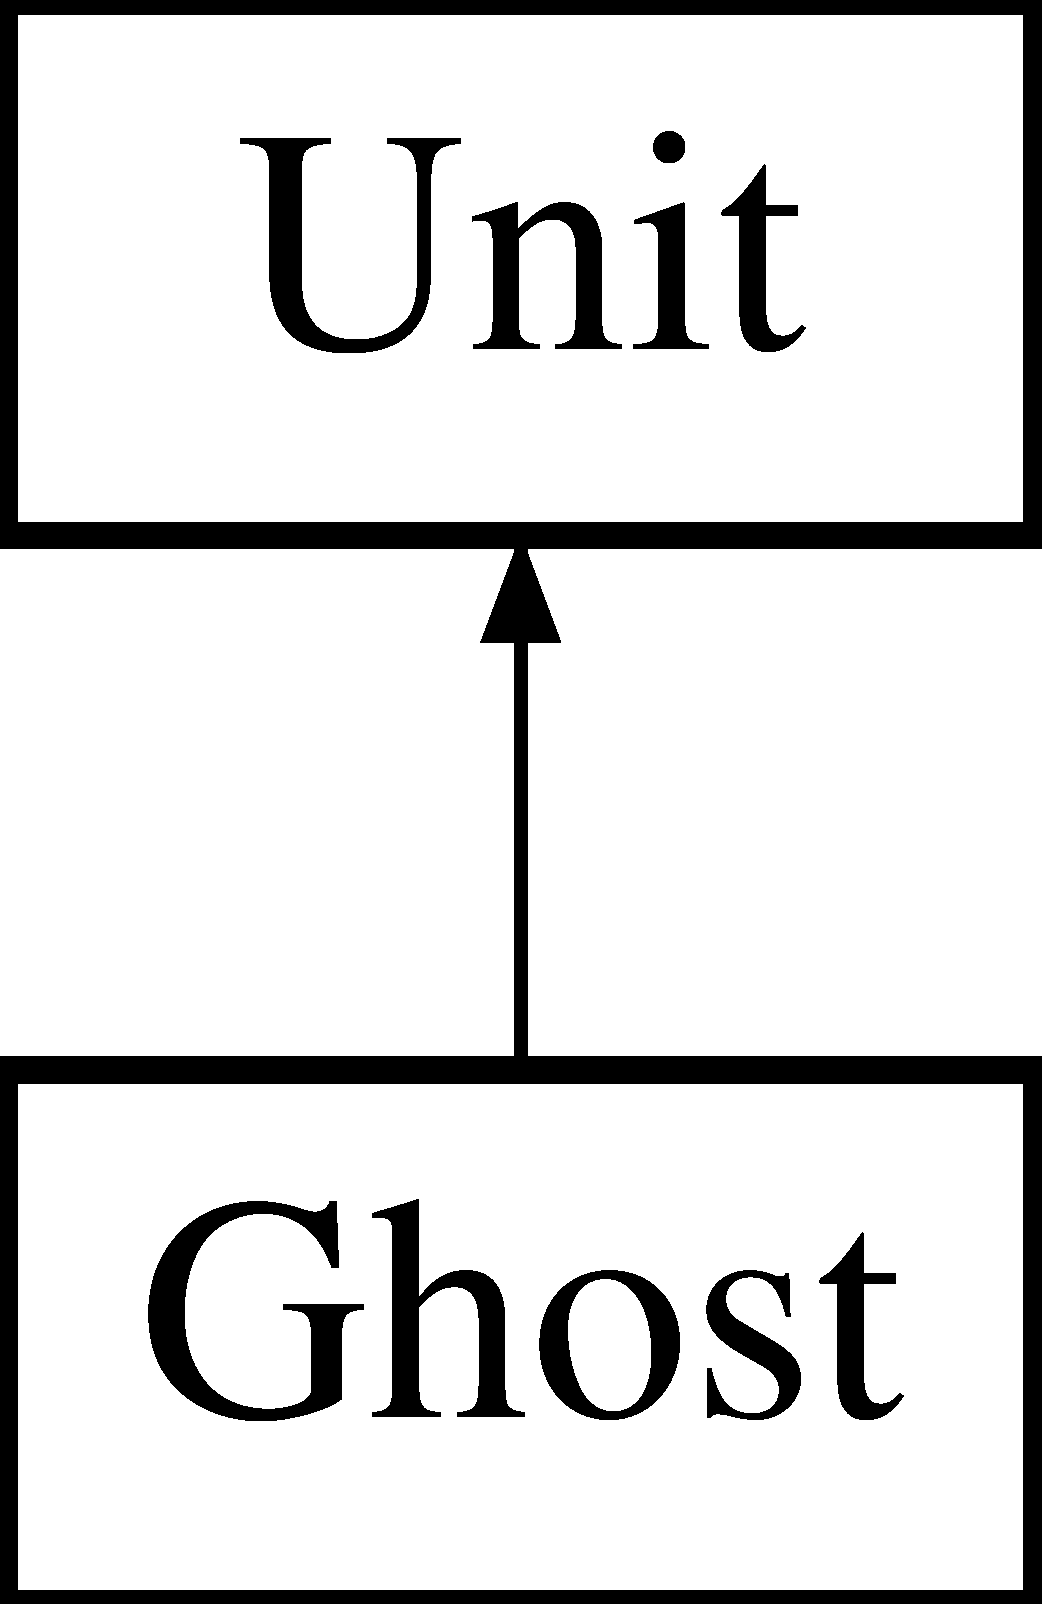
\includegraphics[height=2.000000cm]{class_ghost}
\end{center}
\end{figure}
\subsection*{Public Types}
\begin{DoxyCompactItemize}
\item 
enum \hyperlink{class_ghost_adc8bee2d77e1ca0e4999cace773c71dd}{Ghosts\+I\+D} \{ \hyperlink{class_ghost_adc8bee2d77e1ca0e4999cace773c71dda41f01d04777c489d40e34d6c058c6b5b}{Blinky}, 
\hyperlink{class_ghost_adc8bee2d77e1ca0e4999cace773c71ddac04d44f7968750d812d98cb2b3699cb5}{Pinky}, 
\hyperlink{class_ghost_adc8bee2d77e1ca0e4999cace773c71dda1e770e10aa3bb3f14728210ec28ccf0c}{Inky}, 
\hyperlink{class_ghost_adc8bee2d77e1ca0e4999cace773c71dda28364f0ec8546ed1dea16de59696ab12}{Clyde}
 \}\begin{DoxyCompactList}\small\item\em Identités des fantômes. \end{DoxyCompactList}
\item 
enum \hyperlink{class_ghost_a95bc4313fdf87d827c64fe9607fcc205}{ghost\+Chasing\+Mode\+I\+D} \{ \hyperlink{class_ghost_a95bc4313fdf87d827c64fe9607fcc205a4e0f748a4d226742a8d524f8386fc6db}{Chase}, 
\hyperlink{class_ghost_a95bc4313fdf87d827c64fe9607fcc205a49e7cffc44104e0f3f65579a25804b63}{Scatter}, 
\hyperlink{class_ghost_a95bc4313fdf87d827c64fe9607fcc205ae7975f0b636e971a50a0a4285353ac0e}{Caught}
 \}\begin{DoxyCompactList}\small\item\em Modes de poursuite des fantômes. \end{DoxyCompactList}
\end{DoxyCompactItemize}
\subsection*{Public Member Functions}
\begin{DoxyCompactItemize}
\item 
\hyperlink{class_ghost_a2e38d3c0c8546cceb74777b49a8e3bb7}{Ghost} ()
\begin{DoxyCompactList}\small\item\em Constructeur de base de la classe \hyperlink{class_ghost}{Ghost}. \end{DoxyCompactList}\item 
\hyperlink{class_ghost_a08c2db9f738793076d79de784a17708e}{Ghost} (\hyperlink{class_grid}{Grid} $\ast$grid, int id)
\begin{DoxyCompactList}\small\item\em Surchage du constructeur de base de la classe \hyperlink{class_ghost}{Ghost}. \end{DoxyCompactList}\item 
\hyperlink{class_ghost_ad71ada8752f18eaaccb44ef24b3c8718}{Ghost} (\hyperlink{class_grid}{Grid} $\ast$grid, Q\+Dom\+Element elem, int id)
\begin{DoxyCompactList}\small\item\em Surcharge du constructeur pour utiliser X\+M\+L. \end{DoxyCompactList}\item 
bool \hyperlink{class_ghost_af19dd8db51fe675e626785ebe44a0a1b}{is\+Inside\+Ghost\+House} () const 
\begin{DoxyCompactList}\small\item\em Vérifie si le fantôme se trouve dans la maison définie par sa grille. \end{DoxyCompactList}\item 
\hypertarget{class_ghost_a231a741f4efcc40f47bddb7efa61a19d}{}void \hyperlink{class_ghost_a231a741f4efcc40f47bddb7efa61a19d}{move} ()\label{class_ghost_a231a741f4efcc40f47bddb7efa61a19d}

\begin{DoxyCompactList}\small\item\em Calcule la prochaine position du fantôme en fonction de tous les paramètres et l\textquotesingle{}y déplace. \end{DoxyCompactList}\item 
\hypertarget{class_ghost_aea663d057631b7857e05b26205cb2c4b}{}void \hyperlink{class_ghost_aea663d057631b7857e05b26205cb2c4b}{reverse\+Direction} ()\label{class_ghost_aea663d057631b7857e05b26205cb2c4b}

\begin{DoxyCompactList}\small\item\em Inverse le sens de déplacement du fantôme (lors des changements de mode de poursuite). \end{DoxyCompactList}\item 
int \hyperlink{class_ghost_ac3966bbfe1af0b639d983f20289954f9}{find\+Nextdirection} (Q\+Point tile\+Target, bool ignore\+Previous\+Direction=false)
\begin{DoxyCompactList}\small\item\em Choisit la meilleure direction parmi les options qui s\textquotesingle{}offrent au fantômes. \end{DoxyCompactList}\item 
int \hyperlink{class_ghost_a9aa8db09a42bad7bd62bb336d0b5c89d}{state} () const 
\begin{DoxyCompactList}\small\item\em Getter. \end{DoxyCompactList}\item 
void \hyperlink{class_ghost_a29195fe389663ae6af139466042bd97c}{set\+State} (int \hyperlink{class_ghost_a9aa8db09a42bad7bd62bb336d0b5c89d}{state})
\begin{DoxyCompactList}\small\item\em Modifie l\textquotesingle{}état de poursuite du fantôme. \end{DoxyCompactList}\item 
bool \hyperlink{class_ghost_a990b12906e22b5064e56d3f961f7c2a9}{is\+Free} () const 
\begin{DoxyCompactList}\small\item\em Getter. \end{DoxyCompactList}\item 
void \hyperlink{class_ghost_a8f20887030473a8ceae63f2fe7722a28}{set\+Free} (bool free)
\begin{DoxyCompactList}\small\item\em Setter. \end{DoxyCompactList}\item 
bool \hyperlink{class_ghost_abd3f24e1a2f245865592ba5de5adbcba}{is\+On\+The\+Move} () const 
\begin{DoxyCompactList}\small\item\em Vérifie si la partie réelle de la position du fantôme est nulle. \end{DoxyCompactList}\item 
bool \hyperlink{class_ghost_ae1f2d6e6bbedde18fd5f0465eaf20c08}{is\+Chasing} () const 
\begin{DoxyCompactList}\small\item\em Getter. \end{DoxyCompactList}\item 
bool \hyperlink{class_ghost_aee8ff34fc61b92cc86274fa2b967e814}{is\+Scattering} () const 
\begin{DoxyCompactList}\small\item\em Getter. \end{DoxyCompactList}\item 
\hypertarget{class_ghost_af5702aa6b5aec6edfa9f00843eacd3bb}{}void \hyperlink{class_ghost_af5702aa6b5aec6edfa9f00843eacd3bb}{set\+Caught} ()\label{class_ghost_af5702aa6b5aec6edfa9f00843eacd3bb}

\begin{DoxyCompactList}\small\item\em Marque le fantôme comme attrapé. \end{DoxyCompactList}\item 
bool \hyperlink{class_ghost_adb8eaa0f4a713181fd91f758b7862394}{is\+Caught} () const 
\begin{DoxyCompactList}\small\item\em Getter. \end{DoxyCompactList}\item 
Q\+Point \hyperlink{class_ghost_af538955b257089ee1ab73bcc061b503e}{scatter\+Corner} () const 
\begin{DoxyCompactList}\small\item\em Getter. \end{DoxyCompactList}\item 
Q\+Pixmap \hyperlink{class_ghost_a829efb522dca9924e8228573a08e11c8}{ghost\+Image} (int size=24)
\begin{DoxyCompactList}\small\item\em Dessine l\textquotesingle{}image du fantôme en fonction de ses paramètres (identité, direction, ...). \end{DoxyCompactList}\item 
Q\+Pixmap \hyperlink{class_ghost_a756b09568125dbb619ff93d97ffc9eff}{ghost\+Eyes\+Image} (int size=24)
\begin{DoxyCompactList}\small\item\em Dessine les yeux du fantôme en fonction de sa direction. \end{DoxyCompactList}\end{DoxyCompactItemize}
\subsection*{Static Public Member Functions}
\begin{DoxyCompactItemize}
\item 
static void \hyperlink{class_ghost_adb0d9cf00e0918c43abeb4c1bfc116ec}{set\+Ghosts\+Scared} (bool scared)
\begin{DoxyCompactList}\small\item\em Modifie le comportement en Appeuré ou Normal. \end{DoxyCompactList}\item 
static bool \hyperlink{class_ghost_a09869588955cc6014359262e4f199300}{are\+Ghosts\+Scared} ()
\begin{DoxyCompactList}\small\item\em Getter. \end{DoxyCompactList}\item 
static Q\+Pixmap \hyperlink{class_ghost_a89c202713c5640f09a3cffc73b40d38a}{scared\+Ghost\+Image} (bool flash\+On=false, int size=24)
\begin{DoxyCompactList}\small\item\em Dessine l\textquotesingle{}image d\textquotesingle{}un fantôme effrayé (flashant ou non). \end{DoxyCompactList}\end{DoxyCompactItemize}
\subsection*{Protected Member Functions}
\begin{DoxyCompactItemize}
\item 
\hypertarget{class_ghost_a78fa64d27148af69bd45c57e4261f79d}{}void \hyperlink{class_ghost_a78fa64d27148af69bd45c57e4261f79d}{local\+Move} ()\label{class_ghost_a78fa64d27148af69bd45c57e4261f79d}

\begin{DoxyCompactList}\small\item\em Déplacement au sein d\textquotesingle{}une même case. \end{DoxyCompactList}\item 
\hypertarget{class_ghost_acb51421b22f418d0443a24ae82ca169b}{}void \hyperlink{class_ghost_acb51421b22f418d0443a24ae82ca169b}{chase} ()\label{class_ghost_acb51421b22f418d0443a24ae82ca169b}

\begin{DoxyCompactList}\small\item\em Sélection d\textquotesingle{}une nouvelle direction pour poursuivre le Pacman. \end{DoxyCompactList}\item 
\hypertarget{class_ghost_ad713f0afbe29921b18497972debda803}{}void \hyperlink{class_ghost_ad713f0afbe29921b18497972debda803}{scatter} ()\label{class_ghost_ad713f0afbe29921b18497972debda803}

\begin{DoxyCompactList}\small\item\em Sélection d\textquotesingle{}une nouvelle direction pour aller vers le coin du fantôme. \end{DoxyCompactList}\item 
\hypertarget{class_ghost_a22b8e862c12815a2cfe55bd6583c6a08}{}void \hyperlink{class_ghost_a22b8e862c12815a2cfe55bd6583c6a08}{escape} ()\label{class_ghost_a22b8e862c12815a2cfe55bd6583c6a08}

\begin{DoxyCompactList}\small\item\em Sélection aléatoire d\textquotesingle{}une direction pour fuir le Pacman. \end{DoxyCompactList}\item 
\hypertarget{class_ghost_a0c6d41d57edf393eb20f08eb10457914}{}void \hyperlink{class_ghost_a0c6d41d57edf393eb20f08eb10457914}{go\+Home} ()\label{class_ghost_a0c6d41d57edf393eb20f08eb10457914}

\begin{DoxyCompactList}\small\item\em Sélection d\textquotesingle{}une nouvelle direction vers la maison et saut d\textquotesingle{}une case d\textquotesingle{}un coup. \end{DoxyCompactList}\item 
\hypertarget{class_ghost_a38a8da798ef6876dbbdaa294242f6843}{}void \hyperlink{class_ghost_a38a8da798ef6876dbbdaa294242f6843}{release} ()\label{class_ghost_a38a8da798ef6876dbbdaa294242f6843}

\begin{DoxyCompactList}\small\item\em Libère le fantôme de la maison pour partir à la chasse. \end{DoxyCompactList}\end{DoxyCompactItemize}
\subsection*{Static Protected Member Functions}
\begin{DoxyCompactItemize}
\item 
static Q\+Point \hyperlink{class_ghost_a74121faf86c371e66221fe8d312cb7bf}{blinky\+Chase\+Target} ()
\begin{DoxyCompactList}\small\item\em Getter. \end{DoxyCompactList}\item 
static Q\+Point \hyperlink{class_ghost_a08e782e5437c63edfbfbdc41301c15cc}{pinky\+Chase\+Target} ()
\begin{DoxyCompactList}\small\item\em Getter. \end{DoxyCompactList}\item 
static Q\+Point \hyperlink{class_ghost_a4f4818ff5842e1c640a1edd05aacd8be}{inky\+Chase\+Target} ()
\begin{DoxyCompactList}\small\item\em Getter. \end{DoxyCompactList}\item 
static Q\+Point \hyperlink{class_ghost_aaf68a05af1e6a561e1733b889c35a26b}{clyde\+Chase\+Target} ()
\begin{DoxyCompactList}\small\item\em Getter. \end{DoxyCompactList}\end{DoxyCompactItemize}
\subsection*{Additional Inherited Members}


\subsection{Detailed Description}
Classe d\textquotesingle{}unité de type Fantôme avec les comportements de chaque fantôme. 

\begin{DoxyAuthor}{Author}
Valentin D.\+d.\+G. 
\end{DoxyAuthor}
\begin{DoxyVersion}{Version}
1.\+0
\end{DoxyVersion}
La classe crée dès le lancement du programme les 4 fantômes en variables globales afin d\textquotesingle{}y accéder à partir de n\textquotesingle{}importe où. Les méthodes de la classe permettent aux fantômes d\textquotesingle{}avoir différents comportement, en fonction de leur identité ou de leur état actuel. 

\subsection{Member Enumeration Documentation}
\hypertarget{class_ghost_a95bc4313fdf87d827c64fe9607fcc205}{}\index{Ghost@{Ghost}!ghost\+Chasing\+Mode\+I\+D@{ghost\+Chasing\+Mode\+I\+D}}
\index{ghost\+Chasing\+Mode\+I\+D@{ghost\+Chasing\+Mode\+I\+D}!Ghost@{Ghost}}
\subsubsection[{ghost\+Chasing\+Mode\+I\+D}]{\setlength{\rightskip}{0pt plus 5cm}enum {\bf Ghost\+::ghost\+Chasing\+Mode\+I\+D}}\label{class_ghost_a95bc4313fdf87d827c64fe9607fcc205}


Modes de poursuite des fantômes. 

\begin{Desc}
\item[Enumerator]\par
\begin{description}
\index{Chase@{Chase}!Ghost@{Ghost}}\index{Ghost@{Ghost}!Chase@{Chase}}\item[{\em 
\hypertarget{class_ghost_a95bc4313fdf87d827c64fe9607fcc205a4e0f748a4d226742a8d524f8386fc6db}{}Chase\label{class_ghost_a95bc4313fdf87d827c64fe9607fcc205a4e0f748a4d226742a8d524f8386fc6db}
}]Les fantômes utilisent leur I\+A personnelle pour attraper le Pacman \index{Scatter@{Scatter}!Ghost@{Ghost}}\index{Ghost@{Ghost}!Scatter@{Scatter}}\item[{\em 
\hypertarget{class_ghost_a95bc4313fdf87d827c64fe9607fcc205a49e7cffc44104e0f3f65579a25804b63}{}Scatter\label{class_ghost_a95bc4313fdf87d827c64fe9607fcc205a49e7cffc44104e0f3f65579a25804b63}
}]Les fantômes se dirigent vers leur coin spécifique \index{Caught@{Caught}!Ghost@{Ghost}}\index{Ghost@{Ghost}!Caught@{Caught}}\item[{\em 
\hypertarget{class_ghost_a95bc4313fdf87d827c64fe9607fcc205ae7975f0b636e971a50a0a4285353ac0e}{}Caught\label{class_ghost_a95bc4313fdf87d827c64fe9607fcc205ae7975f0b636e971a50a0a4285353ac0e}
}]Les fantômes attrapés se dirigent vers leur maison et y reste jusqu\textquotesingle{}à expiration \end{description}
\end{Desc}
\hypertarget{class_ghost_adc8bee2d77e1ca0e4999cace773c71dd}{}\index{Ghost@{Ghost}!Ghosts\+I\+D@{Ghosts\+I\+D}}
\index{Ghosts\+I\+D@{Ghosts\+I\+D}!Ghost@{Ghost}}
\subsubsection[{Ghosts\+I\+D}]{\setlength{\rightskip}{0pt plus 5cm}enum {\bf Ghost\+::\+Ghosts\+I\+D}}\label{class_ghost_adc8bee2d77e1ca0e4999cace773c71dd}


Identités des fantômes. 

\begin{Desc}
\item[Enumerator]\par
\begin{description}
\index{Blinky@{Blinky}!Ghost@{Ghost}}\index{Ghost@{Ghost}!Blinky@{Blinky}}\item[{\em 
\hypertarget{class_ghost_adc8bee2d77e1ca0e4999cace773c71dda41f01d04777c489d40e34d6c058c6b5b}{}Blinky\label{class_ghost_adc8bee2d77e1ca0e4999cace773c71dda41f01d04777c489d40e34d6c058c6b5b}
}]Shadow \char`\"{}\+Blinky\char`\"{} \index{Pinky@{Pinky}!Ghost@{Ghost}}\index{Ghost@{Ghost}!Pinky@{Pinky}}\item[{\em 
\hypertarget{class_ghost_adc8bee2d77e1ca0e4999cace773c71ddac04d44f7968750d812d98cb2b3699cb5}{}Pinky\label{class_ghost_adc8bee2d77e1ca0e4999cace773c71ddac04d44f7968750d812d98cb2b3699cb5}
}]Speedy \char`\"{}\+Pinky\char`\"{} \index{Inky@{Inky}!Ghost@{Ghost}}\index{Ghost@{Ghost}!Inky@{Inky}}\item[{\em 
\hypertarget{class_ghost_adc8bee2d77e1ca0e4999cace773c71dda1e770e10aa3bb3f14728210ec28ccf0c}{}Inky\label{class_ghost_adc8bee2d77e1ca0e4999cace773c71dda1e770e10aa3bb3f14728210ec28ccf0c}
}]Bashful \char`\"{}\+Inky\char`\"{} \index{Clyde@{Clyde}!Ghost@{Ghost}}\index{Ghost@{Ghost}!Clyde@{Clyde}}\item[{\em 
\hypertarget{class_ghost_adc8bee2d77e1ca0e4999cace773c71dda28364f0ec8546ed1dea16de59696ab12}{}Clyde\label{class_ghost_adc8bee2d77e1ca0e4999cace773c71dda28364f0ec8546ed1dea16de59696ab12}
}]Pokey \char`\"{}\+Clyde\char`\"{} \end{description}
\end{Desc}


\subsection{Constructor \& Destructor Documentation}
\hypertarget{class_ghost_a2e38d3c0c8546cceb74777b49a8e3bb7}{}\index{Ghost@{Ghost}!Ghost@{Ghost}}
\index{Ghost@{Ghost}!Ghost@{Ghost}}
\subsubsection[{Ghost()}]{\setlength{\rightskip}{0pt plus 5cm}Ghost\+::\+Ghost (
\begin{DoxyParamCaption}
{}
\end{DoxyParamCaption}
)}\label{class_ghost_a2e38d3c0c8546cceb74777b49a8e3bb7}


Constructeur de base de la classe \hyperlink{class_ghost}{Ghost}. 

Note \+: Cette version du constructeur n\textquotesingle{}est pas destinée à être utilisée en dehors de l\textquotesingle{}initialisation d\textquotesingle{}une classe qui la contient. L\textquotesingle{}objet créé n\textquotesingle{}est pas valide. \hypertarget{class_ghost_a08c2db9f738793076d79de784a17708e}{}\index{Ghost@{Ghost}!Ghost@{Ghost}}
\index{Ghost@{Ghost}!Ghost@{Ghost}}
\subsubsection[{Ghost(\+Grid $\ast$grid, int id)}]{\setlength{\rightskip}{0pt plus 5cm}Ghost\+::\+Ghost (
\begin{DoxyParamCaption}
\item[{{\bf Grid} $\ast$}]{grid, }
\item[{int}]{id}
\end{DoxyParamCaption}
)}\label{class_ghost_a08c2db9f738793076d79de784a17708e}


Surchage du constructeur de base de la classe \hyperlink{class_ghost}{Ghost}. 


\begin{DoxyParams}{Parameters}
{\em grid} & La grille sur laquelle se trouve le fantôme. \\
\hline
{\em id} & Identité du fantôme (cf. Ghosts\+I\+D).\\
\hline
\end{DoxyParams}
Un fantôme créé par ce constructeur est valide mais dispose de tous les paramètres par défaut. \hypertarget{class_ghost_ad71ada8752f18eaaccb44ef24b3c8718}{}\index{Ghost@{Ghost}!Ghost@{Ghost}}
\index{Ghost@{Ghost}!Ghost@{Ghost}}
\subsubsection[{Ghost(\+Grid $\ast$grid, Q\+Dom\+Element elem, int id)}]{\setlength{\rightskip}{0pt plus 5cm}Ghost\+::\+Ghost (
\begin{DoxyParamCaption}
\item[{{\bf Grid} $\ast$}]{grid, }
\item[{Q\+Dom\+Element}]{elem, }
\item[{int}]{id}
\end{DoxyParamCaption}
)}\label{class_ghost_ad71ada8752f18eaaccb44ef24b3c8718}


Surcharge du constructeur pour utiliser X\+M\+L. 


\begin{DoxyParams}{Parameters}
{\em grid} & La grille sur laquelle se trouve le fantôme. \\
\hline
{\em elem} & Données X\+M\+L à charger lors de la contruction de l\textquotesingle{}objet. \\
\hline
{\em id} & Identité du fantôme (cf. Ghosts\+I\+D).\\
\hline
\end{DoxyParams}
Construit un fantôme attachée à une grille et dont les paramètres sont chargés à partir d\textquotesingle{}une balise X\+M\+L.
\begin{DoxyItemize}
\item speed \+: Vitesse par défaut de l\textquotesingle{}unité.
\item sspeed \+: Vitesse lorsque les fantômes sont apeurés.
\item cornerx \+: Coordonnée horizontale du coin du fantôme.
\item cornery \+: Coordonnée verticale du coin du fantôme.
\item Autres \+: Voir \hyperlink{class_double_position}{Double\+Position(\+Q\+Dom\+Element elem)}.
\end{DoxyItemize}

Les vitesses doivent être proches d\textquotesingle{}un multiple de M\+A\+X\+\_\+\+F\+L\+O\+A\+T\+\_\+\+P\+O\+S. Par exemple, avec M\+A\+X\+\_\+\+F\+L\+O\+A\+T\+\_\+\+P\+O\+S égal à 1000, 80 donne un résultat assez éloigné (80$\ast$12 = 960, 80$\ast$13 = 1040) alors que 91 donne une valeur très proche (91$\ast$11 = 1001). Si la valeur est trop éloignée, les unités auront des erreurs dans leur déplacement. De base, l\textquotesingle{}écart maximal absolu est de 25.

A la construction, l\textquotesingle{}élément X\+M\+L doit aussi contenir la position qu\textquotesingle{}aura l\textquotesingle{}unité.

Exemple \+: $<$Blinky ix=\char`\"{}13\char`\"{} iy=\char`\"{}11\char`\"{} speed=\char`\"{}71\char`\"{} sspeed = \char`\"{}50\char`\"{} cornerx=\char`\"{}26\char`\"{} cornery=\char`\"{}-\/2\char`\"{} fx = \char`\"{}half\char`\"{}/$>$ 

\subsection{Member Function Documentation}
\hypertarget{class_ghost_a09869588955cc6014359262e4f199300}{}\index{Ghost@{Ghost}!are\+Ghosts\+Scared@{are\+Ghosts\+Scared}}
\index{are\+Ghosts\+Scared@{are\+Ghosts\+Scared}!Ghost@{Ghost}}
\subsubsection[{are\+Ghosts\+Scared()}]{\setlength{\rightskip}{0pt plus 5cm}bool Ghost\+::are\+Ghosts\+Scared (
\begin{DoxyParamCaption}
{}
\end{DoxyParamCaption}
)\hspace{0.3cm}{\ttfamily [static]}}\label{class_ghost_a09869588955cc6014359262e4f199300}


Getter. 

\begin{DoxyReturn}{Returns}
true si les fantômes sont appeurés, sinon false. 
\end{DoxyReturn}
\hypertarget{class_ghost_a74121faf86c371e66221fe8d312cb7bf}{}\index{Ghost@{Ghost}!blinky\+Chase\+Target@{blinky\+Chase\+Target}}
\index{blinky\+Chase\+Target@{blinky\+Chase\+Target}!Ghost@{Ghost}}
\subsubsection[{blinky\+Chase\+Target()}]{\setlength{\rightskip}{0pt plus 5cm}Q\+Point Ghost\+::blinky\+Chase\+Target (
\begin{DoxyParamCaption}
{}
\end{DoxyParamCaption}
)\hspace{0.3cm}{\ttfamily [static]}, {\ttfamily [protected]}}\label{class_ghost_a74121faf86c371e66221fe8d312cb7bf}


Getter. 

\begin{DoxyReturn}{Returns}
Cible de Blinky 
\end{DoxyReturn}
\hypertarget{class_ghost_aaf68a05af1e6a561e1733b889c35a26b}{}\index{Ghost@{Ghost}!clyde\+Chase\+Target@{clyde\+Chase\+Target}}
\index{clyde\+Chase\+Target@{clyde\+Chase\+Target}!Ghost@{Ghost}}
\subsubsection[{clyde\+Chase\+Target()}]{\setlength{\rightskip}{0pt plus 5cm}Q\+Point Ghost\+::clyde\+Chase\+Target (
\begin{DoxyParamCaption}
{}
\end{DoxyParamCaption}
)\hspace{0.3cm}{\ttfamily [static]}, {\ttfamily [protected]}}\label{class_ghost_aaf68a05af1e6a561e1733b889c35a26b}


Getter. 

\begin{DoxyReturn}{Returns}
Cible de Clyde 
\end{DoxyReturn}
\hypertarget{class_ghost_ac3966bbfe1af0b639d983f20289954f9}{}\index{Ghost@{Ghost}!find\+Nextdirection@{find\+Nextdirection}}
\index{find\+Nextdirection@{find\+Nextdirection}!Ghost@{Ghost}}
\subsubsection[{find\+Nextdirection(\+Q\+Point tile\+Target, bool ignore\+Previous\+Direction=false)}]{\setlength{\rightskip}{0pt plus 5cm}int Ghost\+::find\+Nextdirection (
\begin{DoxyParamCaption}
\item[{Q\+Point}]{tile\+Target, }
\item[{bool}]{ignore\+Previous\+Direction = {\ttfamily false}}
\end{DoxyParamCaption}
)}\label{class_ghost_ac3966bbfe1af0b639d983f20289954f9}


Choisit la meilleure direction parmi les options qui s\textquotesingle{}offrent au fantômes. 


\begin{DoxyParams}{Parameters}
{\em tile\+Target} & Cible pour trouver la meilleure direction. \\
\hline
{\em ignore\+Previous\+Direction} & false de base. Si true, le fantôme ignore le fait qu\textquotesingle{}il n\textquotesingle{}a pas le droit de se retourner en temps normal. \\
\hline
\end{DoxyParams}
\begin{DoxyReturn}{Returns}
Meilleure direction à suivre (cf. \hyperlink{class_unit_a198e5fe8c952e2f1e7e9524a914aa0ed}{Unit\+::\+Directions}).
\end{DoxyReturn}
Le fantôme regarde les quatres cases qui l\textquotesingle{}entourent et empile celles où il peut se déplacer.

Ensuite il cherche celle dans la pile qui a la plus courte distance euclidienne vers la cible.

En temps normal, un fantôme ne peut pas se retourner ni se déplacer sur une case avec la collision activée. \hypertarget{class_ghost_a756b09568125dbb619ff93d97ffc9eff}{}\index{Ghost@{Ghost}!ghost\+Eyes\+Image@{ghost\+Eyes\+Image}}
\index{ghost\+Eyes\+Image@{ghost\+Eyes\+Image}!Ghost@{Ghost}}
\subsubsection[{ghost\+Eyes\+Image(int size=24)}]{\setlength{\rightskip}{0pt plus 5cm}Q\+Pixmap Ghost\+::ghost\+Eyes\+Image (
\begin{DoxyParamCaption}
\item[{int}]{size = {\ttfamily 24}}
\end{DoxyParamCaption}
)}\label{class_ghost_a756b09568125dbb619ff93d97ffc9eff}


Dessine les yeux du fantôme en fonction de sa direction. 


\begin{DoxyParams}{Parameters}
{\em size} & Taille de l\textquotesingle{}image finale. \\
\hline
\end{DoxyParams}
\begin{DoxyReturn}{Returns}
Images des yeux du fantôme. 
\end{DoxyReturn}
\hypertarget{class_ghost_a829efb522dca9924e8228573a08e11c8}{}\index{Ghost@{Ghost}!ghost\+Image@{ghost\+Image}}
\index{ghost\+Image@{ghost\+Image}!Ghost@{Ghost}}
\subsubsection[{ghost\+Image(int size=24)}]{\setlength{\rightskip}{0pt plus 5cm}Q\+Pixmap Ghost\+::ghost\+Image (
\begin{DoxyParamCaption}
\item[{int}]{size = {\ttfamily 24}}
\end{DoxyParamCaption}
)}\label{class_ghost_a829efb522dca9924e8228573a08e11c8}


Dessine l\textquotesingle{}image du fantôme en fonction de ses paramètres (identité, direction, ...). 


\begin{DoxyParams}{Parameters}
{\em size} & Taille de l\textquotesingle{}image du fantôme. \\
\hline
\end{DoxyParams}
\begin{DoxyReturn}{Returns}
Image finale du fantôme. 
\end{DoxyReturn}
\hypertarget{class_ghost_a4f4818ff5842e1c640a1edd05aacd8be}{}\index{Ghost@{Ghost}!inky\+Chase\+Target@{inky\+Chase\+Target}}
\index{inky\+Chase\+Target@{inky\+Chase\+Target}!Ghost@{Ghost}}
\subsubsection[{inky\+Chase\+Target()}]{\setlength{\rightskip}{0pt plus 5cm}Q\+Point Ghost\+::inky\+Chase\+Target (
\begin{DoxyParamCaption}
{}
\end{DoxyParamCaption}
)\hspace{0.3cm}{\ttfamily [static]}, {\ttfamily [protected]}}\label{class_ghost_a4f4818ff5842e1c640a1edd05aacd8be}


Getter. 

\begin{DoxyReturn}{Returns}
Cible de Inky 
\end{DoxyReturn}
\hypertarget{class_ghost_adb8eaa0f4a713181fd91f758b7862394}{}\index{Ghost@{Ghost}!is\+Caught@{is\+Caught}}
\index{is\+Caught@{is\+Caught}!Ghost@{Ghost}}
\subsubsection[{is\+Caught() const }]{\setlength{\rightskip}{0pt plus 5cm}bool Ghost\+::is\+Caught (
\begin{DoxyParamCaption}
{}
\end{DoxyParamCaption}
) const}\label{class_ghost_adb8eaa0f4a713181fd91f758b7862394}


Getter. 

\begin{DoxyReturn}{Returns}
true si le fantôme est attrapé, false sinon. 
\end{DoxyReturn}
\hypertarget{class_ghost_ae1f2d6e6bbedde18fd5f0465eaf20c08}{}\index{Ghost@{Ghost}!is\+Chasing@{is\+Chasing}}
\index{is\+Chasing@{is\+Chasing}!Ghost@{Ghost}}
\subsubsection[{is\+Chasing() const }]{\setlength{\rightskip}{0pt plus 5cm}bool Ghost\+::is\+Chasing (
\begin{DoxyParamCaption}
{}
\end{DoxyParamCaption}
) const}\label{class_ghost_ae1f2d6e6bbedde18fd5f0465eaf20c08}


Getter. 

\begin{DoxyReturn}{Returns}
true si l\textquotesingle{}état est à Chase, sinon false. 
\end{DoxyReturn}
\hypertarget{class_ghost_a990b12906e22b5064e56d3f961f7c2a9}{}\index{Ghost@{Ghost}!is\+Free@{is\+Free}}
\index{is\+Free@{is\+Free}!Ghost@{Ghost}}
\subsubsection[{is\+Free() const }]{\setlength{\rightskip}{0pt plus 5cm}bool Ghost\+::is\+Free (
\begin{DoxyParamCaption}
{}
\end{DoxyParamCaption}
) const}\label{class_ghost_a990b12906e22b5064e56d3f961f7c2a9}


Getter. 

\begin{DoxyReturn}{Returns}
true si le fantôme a le droit de sortir.
\end{DoxyReturn}
De base, seuls Blinky et Pinky sont capables de sortir. Inky attend que Pacman ait mangé 30 pastilles et Clyde attend qu\textquotesingle{}il en ai mangé un tiers. \hypertarget{class_ghost_af19dd8db51fe675e626785ebe44a0a1b}{}\index{Ghost@{Ghost}!is\+Inside\+Ghost\+House@{is\+Inside\+Ghost\+House}}
\index{is\+Inside\+Ghost\+House@{is\+Inside\+Ghost\+House}!Ghost@{Ghost}}
\subsubsection[{is\+Inside\+Ghost\+House() const }]{\setlength{\rightskip}{0pt plus 5cm}bool Ghost\+::is\+Inside\+Ghost\+House (
\begin{DoxyParamCaption}
{}
\end{DoxyParamCaption}
) const}\label{class_ghost_af19dd8db51fe675e626785ebe44a0a1b}


Vérifie si le fantôme se trouve dans la maison définie par sa grille. 

\begin{DoxyReturn}{Returns}
true si le fantôme se trouve dans la maison, sinon false. 
\end{DoxyReturn}
\hypertarget{class_ghost_abd3f24e1a2f245865592ba5de5adbcba}{}\index{Ghost@{Ghost}!is\+On\+The\+Move@{is\+On\+The\+Move}}
\index{is\+On\+The\+Move@{is\+On\+The\+Move}!Ghost@{Ghost}}
\subsubsection[{is\+On\+The\+Move() const }]{\setlength{\rightskip}{0pt plus 5cm}bool Ghost\+::is\+On\+The\+Move (
\begin{DoxyParamCaption}
{}
\end{DoxyParamCaption}
) const}\label{class_ghost_abd3f24e1a2f245865592ba5de5adbcba}


Vérifie si la partie réelle de la position du fantôme est nulle. 

\begin{DoxyReturn}{Returns}
true si la partie réelle n\textquotesingle{}est pas nulle, sinon false. 
\end{DoxyReturn}
\hypertarget{class_ghost_aee8ff34fc61b92cc86274fa2b967e814}{}\index{Ghost@{Ghost}!is\+Scattering@{is\+Scattering}}
\index{is\+Scattering@{is\+Scattering}!Ghost@{Ghost}}
\subsubsection[{is\+Scattering() const }]{\setlength{\rightskip}{0pt plus 5cm}bool Ghost\+::is\+Scattering (
\begin{DoxyParamCaption}
{}
\end{DoxyParamCaption}
) const}\label{class_ghost_aee8ff34fc61b92cc86274fa2b967e814}


Getter. 

\begin{DoxyReturn}{Returns}
true si l\textquotesingle{}état est à Scatter, sinon false. 
\end{DoxyReturn}
\hypertarget{class_ghost_a08e782e5437c63edfbfbdc41301c15cc}{}\index{Ghost@{Ghost}!pinky\+Chase\+Target@{pinky\+Chase\+Target}}
\index{pinky\+Chase\+Target@{pinky\+Chase\+Target}!Ghost@{Ghost}}
\subsubsection[{pinky\+Chase\+Target()}]{\setlength{\rightskip}{0pt plus 5cm}Q\+Point Ghost\+::pinky\+Chase\+Target (
\begin{DoxyParamCaption}
{}
\end{DoxyParamCaption}
)\hspace{0.3cm}{\ttfamily [static]}, {\ttfamily [protected]}}\label{class_ghost_a08e782e5437c63edfbfbdc41301c15cc}


Getter. 

\begin{DoxyReturn}{Returns}
Cible de Pinky 
\end{DoxyReturn}
\hypertarget{class_ghost_a89c202713c5640f09a3cffc73b40d38a}{}\index{Ghost@{Ghost}!scared\+Ghost\+Image@{scared\+Ghost\+Image}}
\index{scared\+Ghost\+Image@{scared\+Ghost\+Image}!Ghost@{Ghost}}
\subsubsection[{scared\+Ghost\+Image(bool flash\+On=false, int size=24)}]{\setlength{\rightskip}{0pt plus 5cm}Q\+Pixmap Ghost\+::scared\+Ghost\+Image (
\begin{DoxyParamCaption}
\item[{bool}]{flash\+On = {\ttfamily false}, }
\item[{int}]{size = {\ttfamily 24}}
\end{DoxyParamCaption}
)\hspace{0.3cm}{\ttfamily [static]}}\label{class_ghost_a89c202713c5640f09a3cffc73b40d38a}


Dessine l\textquotesingle{}image d\textquotesingle{}un fantôme effrayé (flashant ou non). 


\begin{DoxyParams}{Parameters}
{\em flash\+On} & Si true, alors le fantôme est blanc, sinon bleu foncé. \\
\hline
{\em size} & Taille de l\textquotesingle{}image finale. \\
\hline
\end{DoxyParams}
\begin{DoxyReturn}{Returns}
Image de fantôme effrayé. 
\end{DoxyReturn}
\hypertarget{class_ghost_af538955b257089ee1ab73bcc061b503e}{}\index{Ghost@{Ghost}!scatter\+Corner@{scatter\+Corner}}
\index{scatter\+Corner@{scatter\+Corner}!Ghost@{Ghost}}
\subsubsection[{scatter\+Corner() const }]{\setlength{\rightskip}{0pt plus 5cm}Q\+Point Ghost\+::scatter\+Corner (
\begin{DoxyParamCaption}
{}
\end{DoxyParamCaption}
) const}\label{class_ghost_af538955b257089ee1ab73bcc061b503e}


Getter. 

\begin{DoxyReturn}{Returns}
Le coin du mode Scatter du fantôme. 
\end{DoxyReturn}
\hypertarget{class_ghost_a8f20887030473a8ceae63f2fe7722a28}{}\index{Ghost@{Ghost}!set\+Free@{set\+Free}}
\index{set\+Free@{set\+Free}!Ghost@{Ghost}}
\subsubsection[{set\+Free(bool free)}]{\setlength{\rightskip}{0pt plus 5cm}void Ghost\+::set\+Free (
\begin{DoxyParamCaption}
\item[{bool}]{free}
\end{DoxyParamCaption}
)}\label{class_ghost_a8f20887030473a8ceae63f2fe7722a28}


Setter. 


\begin{DoxyParams}{Parameters}
{\em free} & Si true alors le fantôme devient capable de sortir de la maison et démarre son I\+A. \\
\hline
\end{DoxyParams}
\hypertarget{class_ghost_adb0d9cf00e0918c43abeb4c1bfc116ec}{}\index{Ghost@{Ghost}!set\+Ghosts\+Scared@{set\+Ghosts\+Scared}}
\index{set\+Ghosts\+Scared@{set\+Ghosts\+Scared}!Ghost@{Ghost}}
\subsubsection[{set\+Ghosts\+Scared(bool scared)}]{\setlength{\rightskip}{0pt plus 5cm}void Ghost\+::set\+Ghosts\+Scared (
\begin{DoxyParamCaption}
\item[{bool}]{scared}
\end{DoxyParamCaption}
)\hspace{0.3cm}{\ttfamily [static]}}\label{class_ghost_adb0d9cf00e0918c43abeb4c1bfc116ec}


Modifie le comportement en Appeuré ou Normal. 


\begin{DoxyParams}{Parameters}
{\em scared} & Si true, alors le comportement devient Appeuré sinon Normal. \\
\hline
\end{DoxyParams}
\hypertarget{class_ghost_a29195fe389663ae6af139466042bd97c}{}\index{Ghost@{Ghost}!set\+State@{set\+State}}
\index{set\+State@{set\+State}!Ghost@{Ghost}}
\subsubsection[{set\+State(int state)}]{\setlength{\rightskip}{0pt plus 5cm}void Ghost\+::set\+State (
\begin{DoxyParamCaption}
\item[{int}]{state}
\end{DoxyParamCaption}
)}\label{class_ghost_a29195fe389663ae6af139466042bd97c}


Modifie l\textquotesingle{}état de poursuite du fantôme. 


\begin{DoxyParams}{Parameters}
{\em state} & Nouvel état de poursuite. \\
\hline
\end{DoxyParams}
\hypertarget{class_ghost_a9aa8db09a42bad7bd62bb336d0b5c89d}{}\index{Ghost@{Ghost}!state@{state}}
\index{state@{state}!Ghost@{Ghost}}
\subsubsection[{state() const }]{\setlength{\rightskip}{0pt plus 5cm}int Ghost\+::state (
\begin{DoxyParamCaption}
{}
\end{DoxyParamCaption}
) const}\label{class_ghost_a9aa8db09a42bad7bd62bb336d0b5c89d}


Getter. 

\begin{DoxyReturn}{Returns}
Etat de poursuite actuel du fantôme.(cf. ghost\+Chasing\+Mode\+I\+D). 
\end{DoxyReturn}


The documentation for this class was generated from the following files\+:\begin{DoxyCompactItemize}
\item 
ghost.\+h\item 
ghost.\+cpp\end{DoxyCompactItemize}

\hypertarget{class_ghost_timer}{}\section{Ghost\+Timer Class Reference}
\label{class_ghost_timer}\index{Ghost\+Timer@{Ghost\+Timer}}


Classe de Timer pour les modes des fantômes.  




{\ttfamily \#include $<$ghosttimer.\+h$>$}

\subsection*{Public Member Functions}
\begin{DoxyCompactItemize}
\item 
\hyperlink{class_ghost_timer_adebf7cf8bb544e23f6fd8ce7095b8394}{Ghost\+Timer} ()
\begin{DoxyCompactList}\small\item\em Constructeur de base de la classe \hyperlink{class_ghost_timer}{Ghost\+Timer}. \end{DoxyCompactList}\item 
\hyperlink{class_ghost_timer_a363147268fa53ea5e7f9e4b50b8453ef}{Ghost\+Timer} (Q\+Dom\+Element elem)
\begin{DoxyCompactList}\small\item\em Surcharge du constructeur pour utiliser X\+M\+L. \end{DoxyCompactList}\item 
int \hyperlink{class_ghost_timer_adf6ae0f333a95d4fe3e6f8a132a8201d}{current\+Mode} () const 
\begin{DoxyCompactList}\small\item\em Getter. \end{DoxyCompactList}\item 
void \hyperlink{class_ghost_timer_acca62ab4734e961d46965a7d10a886ad}{increase\+Timer} ()
\begin{DoxyCompactList}\small\item\em Augmente la valeur du timer de T\+I\+M\+E\+\_\+\+B\+E\+T\+W\+E\+E\+N\+\_\+\+F\+R\+A\+M\+E\+S mscs. \end{DoxyCompactList}\end{DoxyCompactItemize}


\subsection{Detailed Description}
Classe de Timer pour les modes des fantômes. 

\begin{DoxyAuthor}{Author}
Valentin D.\+d.\+G. 
\end{DoxyAuthor}
\begin{DoxyVersion}{Version}
1.\+0
\end{DoxyVersion}
Cette classe permet de suivre le mode de poursuite des fantômes en fonction du temps écoulé dans la partie.

Il est nécessaire d\textquotesingle{}appeler manuellement la fonction de mise à jour du timer. 

\subsection{Constructor \& Destructor Documentation}
\hypertarget{class_ghost_timer_adebf7cf8bb544e23f6fd8ce7095b8394}{}\index{Ghost\+Timer@{Ghost\+Timer}!Ghost\+Timer@{Ghost\+Timer}}
\index{Ghost\+Timer@{Ghost\+Timer}!Ghost\+Timer@{Ghost\+Timer}}
\subsubsection[{Ghost\+Timer()}]{\setlength{\rightskip}{0pt plus 5cm}Ghost\+Timer\+::\+Ghost\+Timer (
\begin{DoxyParamCaption}
{}
\end{DoxyParamCaption}
)}\label{class_ghost_timer_adebf7cf8bb544e23f6fd8ce7095b8394}


Constructeur de base de la classe \hyperlink{class_ghost_timer}{Ghost\+Timer}. 

Note \+: Cette version du constructeur n\textquotesingle{}est pas destinée à être utilisée en dehors de l\textquotesingle{}initialisation d\textquotesingle{}une classe qui la contient. L\textquotesingle{}objet créé n\textquotesingle{}est pas valide. \hypertarget{class_ghost_timer_a363147268fa53ea5e7f9e4b50b8453ef}{}\index{Ghost\+Timer@{Ghost\+Timer}!Ghost\+Timer@{Ghost\+Timer}}
\index{Ghost\+Timer@{Ghost\+Timer}!Ghost\+Timer@{Ghost\+Timer}}
\subsubsection[{Ghost\+Timer(\+Q\+Dom\+Element elem)}]{\setlength{\rightskip}{0pt plus 5cm}Ghost\+Timer\+::\+Ghost\+Timer (
\begin{DoxyParamCaption}
\item[{Q\+Dom\+Element}]{elem}
\end{DoxyParamCaption}
)}\label{class_ghost_timer_a363147268fa53ea5e7f9e4b50b8453ef}


Surcharge du constructeur pour utiliser X\+M\+L. 


\begin{DoxyParams}{Parameters}
{\em elem} & Données X\+M\+L à charger lors de la contruction de l\textquotesingle{}objet.\\
\hline
\end{DoxyParams}
L\textquotesingle{}élément X\+M\+L doit ressembler au template suivant \+:
\begin{DoxyItemize}
\item $<$\hyperlink{class_ghost_timer}{Ghost\+Timer}$>$
\begin{DoxyItemize}
\item $<$Step time=\char`\"{}7\char`\"{} mode=\char`\"{}0\char`\"{}/$>$ // Mode Scatter (0) pendant 7 secondes.
\item $<$Step time=\char`\"{}20\char`\"{} mode=\char`\"{}1\char`\"{}/$>$ // Puis Chase(1) pendant 20 secondes.
\item $<$Step time=\char`\"{}7\char`\"{} mode=\char`\"{}0\char`\"{}/$>$ // Puis Scatter (0) jusqu\textquotesingle{}à la fin (time ignoré).
\end{DoxyItemize}
\item $<$/\+Ghost\+Timer$>$ 
\end{DoxyItemize}

\subsection{Member Function Documentation}
\hypertarget{class_ghost_timer_adf6ae0f333a95d4fe3e6f8a132a8201d}{}\index{Ghost\+Timer@{Ghost\+Timer}!current\+Mode@{current\+Mode}}
\index{current\+Mode@{current\+Mode}!Ghost\+Timer@{Ghost\+Timer}}
\subsubsection[{current\+Mode() const }]{\setlength{\rightskip}{0pt plus 5cm}int Ghost\+Timer\+::current\+Mode (
\begin{DoxyParamCaption}
{}
\end{DoxyParamCaption}
) const}\label{class_ghost_timer_adf6ae0f333a95d4fe3e6f8a132a8201d}


Getter. 

\begin{DoxyReturn}{Returns}
Mode de poursuite actuel du timer. 
\end{DoxyReturn}
\hypertarget{class_ghost_timer_acca62ab4734e961d46965a7d10a886ad}{}\index{Ghost\+Timer@{Ghost\+Timer}!increase\+Timer@{increase\+Timer}}
\index{increase\+Timer@{increase\+Timer}!Ghost\+Timer@{Ghost\+Timer}}
\subsubsection[{increase\+Timer()}]{\setlength{\rightskip}{0pt plus 5cm}void Ghost\+Timer\+::increase\+Timer (
\begin{DoxyParamCaption}
{}
\end{DoxyParamCaption}
)}\label{class_ghost_timer_acca62ab4734e961d46965a7d10a886ad}


Augmente la valeur du timer de T\+I\+M\+E\+\_\+\+B\+E\+T\+W\+E\+E\+N\+\_\+\+F\+R\+A\+M\+E\+S mscs. 

Si la valeur excède la prochaine limite de temps, le timer passe au prochain mode et réinitialise sa valeur de temps. 

The documentation for this class was generated from the following files\+:\begin{DoxyCompactItemize}
\item 
ghosttimer.\+h\item 
ghosttimer.\+cpp\end{DoxyCompactItemize}

\hypertarget{class_grid}{}\section{Grid Class Reference}
\label{class_grid}\index{Grid@{Grid}}


Classe de grille de Pacman.  




{\ttfamily \#include $<$grid.\+h$>$}

\subsection*{Public Types}
\begin{DoxyCompactItemize}
\item 
enum \hyperlink{class_grid_a473f8c5d768a1734d8911bf1213ce10f}{Collisions\+I\+D} \{ \hyperlink{class_grid_a473f8c5d768a1734d8911bf1213ce10fa0a40927bb14a23a6aeb090abe9bfb517}{Collision\+Off}, 
\hyperlink{class_grid_a473f8c5d768a1734d8911bf1213ce10fa2b394e743be772d4a1da354d5b597623}{Collision\+On}
 \}\begin{DoxyCompactList}\small\item\em Types de collisions. \end{DoxyCompactList}
\end{DoxyCompactItemize}
\subsection*{Public Member Functions}
\begin{DoxyCompactItemize}
\item 
\hyperlink{class_grid_a4d98f6e0a0a048fbce5b77fbc0cba646}{Grid} (Q\+Dom\+Element elem, \hyperlink{class_texture_handler}{Texture\+Handler} $\ast$texture\+Handler)
\begin{DoxyCompactList}\small\item\em Constructeur de base de \hyperlink{class_grid}{Grid}. \end{DoxyCompactList}\item 
Q\+Size \hyperlink{class_grid_aa79281119d2e4644d53c9fba286b5dad}{size} () const 
\begin{DoxyCompactList}\small\item\em Getter. \end{DoxyCompactList}\item 
void \hyperlink{class_grid_ad7b1701e7ba881746363ad87aee5c879}{add\+Texture} (Q\+String filename)
\begin{DoxyCompactList}\small\item\em Ajoute la texture à la liste des textures de la grille. \end{DoxyCompactList}\item 
Q\+Pixmap \hyperlink{class_grid_a1e092c1365a7e1759a169de4e305c777}{texture\+At} (int index)
\begin{DoxyCompactList}\small\item\em Donne la texture de la liste des textures de la grille à l\textquotesingle{}index donné. \end{DoxyCompactList}\item 
int \hyperlink{class_grid_aeb52c62fd156c4169463d3f6cff8208e}{tile\+Texture} (Q\+Point p)
\begin{DoxyCompactList}\small\item\em Donne le numéro de la texture à la case donnée. \end{DoxyCompactList}\item 
int \hyperlink{class_grid_af6f09b36ec823d16065f2f8c997ba071}{tile\+Texture} (int i)
\begin{DoxyCompactList}\small\item\em Donne le numéro de la texture à la case donnée. \end{DoxyCompactList}\item 
void \hyperlink{class_grid_abf2e8bc6fe111e3228fea6a496befc16}{set\+Tile\+Texture} (Q\+Point p, int texture)
\begin{DoxyCompactList}\small\item\em Modifie la texture à la case donnée. \end{DoxyCompactList}\item 
int \hyperlink{class_grid_af360f3f9d6df547d63829a3af47e5109}{tiles\+Size} () const 
\begin{DoxyCompactList}\small\item\em Getter. \end{DoxyCompactList}\item 
int \hyperlink{class_grid_a711ac8dd739f2fded9160f467be76bf4}{collision\+At} (Q\+Point pos) const 
\begin{DoxyCompactList}\small\item\em Donne la valeur de collision au point donné. \end{DoxyCompactList}\item 
Q\+Pixmap \hyperlink{class_grid_a4a021bb5b8a2210cb8a773ae23131090}{process\+Base\+Image} ()
\begin{DoxyCompactList}\small\item\em Calcule l\textquotesingle{}image de base de la grille. \end{DoxyCompactList}\item 
Q\+Pixmap \hyperlink{class_grid_a6186275b098df986400db17659895b23}{update\+Base\+Image} ()
\begin{DoxyCompactList}\small\item\em Met à jour l\textquotesingle{}image de base de la grille. \end{DoxyCompactList}\item 
Q\+Rect \hyperlink{class_grid_a96c1d1e403aa5e04aeb6b194795448c4}{ghost\+House} () const 
\begin{DoxyCompactList}\small\item\em Getter. \end{DoxyCompactList}\item 
int \hyperlink{class_grid_acc9b139189e4242de864c5bc7a60987c}{empty\+Tile} () const 
\begin{DoxyCompactList}\small\item\em Getter. \end{DoxyCompactList}\item 
void \hyperlink{class_grid_a8c6bd2ddd44b14bf887d5e0bfc7a6fb3}{set\+Empty\+Tile} (int \hyperlink{class_grid_acc9b139189e4242de864c5bc7a60987c}{empty\+Tile})
\begin{DoxyCompactList}\small\item\em Setter. \end{DoxyCompactList}\item 
int \hyperlink{class_grid_a9816017ce1a36bdad4d489383d19acc6}{pellet\+Tile} () const 
\begin{DoxyCompactList}\small\item\em Getter. \end{DoxyCompactList}\item 
void \hyperlink{class_grid_ac97425f75ec6edde70f12a8d2f3b450f}{set\+Pellet\+Tile} (int \hyperlink{class_grid_a9816017ce1a36bdad4d489383d19acc6}{pellet\+Tile})
\begin{DoxyCompactList}\small\item\em Setter. \end{DoxyCompactList}\item 
int \hyperlink{class_grid_afa7b0cbe21203a8bf089ab537510392c}{energizer\+Tile} () const 
\begin{DoxyCompactList}\small\item\em Getter. \end{DoxyCompactList}\item 
void \hyperlink{class_grid_a72e0bb85cb48c443e409b4fdffe8c40c}{set\+Energizer\+Tile} (int \hyperlink{class_grid_afa7b0cbe21203a8bf089ab537510392c}{energizer\+Tile})
\begin{DoxyCompactList}\small\item\em Setter. \end{DoxyCompactList}\end{DoxyCompactItemize}


\subsection{Detailed Description}
Classe de grille de Pacman. 

\begin{DoxyAuthor}{Author}
Valentin D.\+d.\+G. 
\end{DoxyAuthor}
\begin{DoxyVersion}{Version}
1.\+0
\end{DoxyVersion}
La Grille s\textquotesingle{}occupe d\textquotesingle{}attribuer à chaque case une texture et un indicateur de collision.

La classe génère une image de base qui sera mise à jour le minimum possible (une case par frame en théorie) afin d\textquotesingle{}être utilisée par d\textquotesingle{}autres classes ultérieurement. La grille s\textquotesingle{}occupe aussi de baliser la maison des fantômes. 

\subsection{Member Enumeration Documentation}
\hypertarget{class_grid_a473f8c5d768a1734d8911bf1213ce10f}{}\index{Grid@{Grid}!Collisions\+I\+D@{Collisions\+I\+D}}
\index{Collisions\+I\+D@{Collisions\+I\+D}!Grid@{Grid}}
\subsubsection[{Collisions\+I\+D}]{\setlength{\rightskip}{0pt plus 5cm}enum {\bf Grid\+::\+Collisions\+I\+D}}\label{class_grid_a473f8c5d768a1734d8911bf1213ce10f}


Types de collisions. 

\begin{Desc}
\item[Enumerator]\par
\begin{description}
\index{Collision\+Off@{Collision\+Off}!Grid@{Grid}}\index{Grid@{Grid}!Collision\+Off@{Collision\+Off}}\item[{\em 
\hypertarget{class_grid_a473f8c5d768a1734d8911bf1213ce10fa0a40927bb14a23a6aeb090abe9bfb517}{}Collision\+Off\label{class_grid_a473f8c5d768a1734d8911bf1213ce10fa0a40927bb14a23a6aeb090abe9bfb517}
}]Collision désactivée \index{Collision\+On@{Collision\+On}!Grid@{Grid}}\index{Grid@{Grid}!Collision\+On@{Collision\+On}}\item[{\em 
\hypertarget{class_grid_a473f8c5d768a1734d8911bf1213ce10fa2b394e743be772d4a1da354d5b597623}{}Collision\+On\label{class_grid_a473f8c5d768a1734d8911bf1213ce10fa2b394e743be772d4a1da354d5b597623}
}]Collision activée \end{description}
\end{Desc}


\subsection{Constructor \& Destructor Documentation}
\hypertarget{class_grid_a4d98f6e0a0a048fbce5b77fbc0cba646}{}\index{Grid@{Grid}!Grid@{Grid}}
\index{Grid@{Grid}!Grid@{Grid}}
\subsubsection[{Grid(\+Q\+Dom\+Element elem, Texture\+Handler $\ast$texture\+Handler)}]{\setlength{\rightskip}{0pt plus 5cm}Grid\+::\+Grid (
\begin{DoxyParamCaption}
\item[{Q\+Dom\+Element}]{elem, }
\item[{{\bf Texture\+Handler} $\ast$}]{texture\+Handler}
\end{DoxyParamCaption}
)}\label{class_grid_a4d98f6e0a0a048fbce5b77fbc0cba646}


Constructeur de base de \hyperlink{class_grid}{Grid}. 


\begin{DoxyParams}{Parameters}
{\em elem} & Données X\+M\+L à charger lors de la contruction de l\textquotesingle{}objet. \\
\hline
{\em texture\+Handler} & Gestionnaire de texture déjà instancié d\textquotesingle{}où la grille va extraire les textures. \\
\hline
\end{DoxyParams}


\subsection{Member Function Documentation}
\hypertarget{class_grid_ad7b1701e7ba881746363ad87aee5c879}{}\index{Grid@{Grid}!add\+Texture@{add\+Texture}}
\index{add\+Texture@{add\+Texture}!Grid@{Grid}}
\subsubsection[{add\+Texture(\+Q\+String filename)}]{\setlength{\rightskip}{0pt plus 5cm}void Grid\+::add\+Texture (
\begin{DoxyParamCaption}
\item[{Q\+String}]{filename}
\end{DoxyParamCaption}
)}\label{class_grid_ad7b1701e7ba881746363ad87aee5c879}


Ajoute la texture à la liste des textures de la grille. 


\begin{DoxyParams}{Parameters}
{\em filename} & Chemin vers la texture \\
\hline
\end{DoxyParams}
\hypertarget{class_grid_a711ac8dd739f2fded9160f467be76bf4}{}\index{Grid@{Grid}!collision\+At@{collision\+At}}
\index{collision\+At@{collision\+At}!Grid@{Grid}}
\subsubsection[{collision\+At(\+Q\+Point pos) const }]{\setlength{\rightskip}{0pt plus 5cm}int Grid\+::collision\+At (
\begin{DoxyParamCaption}
\item[{Q\+Point}]{pos}
\end{DoxyParamCaption}
) const}\label{class_grid_a711ac8dd739f2fded9160f467be76bf4}


Donne la valeur de collision au point donné. 


\begin{DoxyParams}{Parameters}
{\em pos} & Case à inspecter. \\
\hline
\end{DoxyParams}
\begin{DoxyReturn}{Returns}
Valeur de collision. 
\end{DoxyReturn}
\hypertarget{class_grid_acc9b139189e4242de864c5bc7a60987c}{}\index{Grid@{Grid}!empty\+Tile@{empty\+Tile}}
\index{empty\+Tile@{empty\+Tile}!Grid@{Grid}}
\subsubsection[{empty\+Tile() const }]{\setlength{\rightskip}{0pt plus 5cm}int Grid\+::empty\+Tile (
\begin{DoxyParamCaption}
{}
\end{DoxyParamCaption}
) const}\label{class_grid_acc9b139189e4242de864c5bc7a60987c}


Getter. 

\begin{DoxyReturn}{Returns}
Numero de case vide. 
\end{DoxyReturn}
\hypertarget{class_grid_afa7b0cbe21203a8bf089ab537510392c}{}\index{Grid@{Grid}!energizer\+Tile@{energizer\+Tile}}
\index{energizer\+Tile@{energizer\+Tile}!Grid@{Grid}}
\subsubsection[{energizer\+Tile() const }]{\setlength{\rightskip}{0pt plus 5cm}int Grid\+::energizer\+Tile (
\begin{DoxyParamCaption}
{}
\end{DoxyParamCaption}
) const}\label{class_grid_afa7b0cbe21203a8bf089ab537510392c}


Getter. 

\begin{DoxyReturn}{Returns}
Numero de case avec énergisant. 
\end{DoxyReturn}
\hypertarget{class_grid_a96c1d1e403aa5e04aeb6b194795448c4}{}\index{Grid@{Grid}!ghost\+House@{ghost\+House}}
\index{ghost\+House@{ghost\+House}!Grid@{Grid}}
\subsubsection[{ghost\+House() const }]{\setlength{\rightskip}{0pt plus 5cm}Q\+Rect Grid\+::ghost\+House (
\begin{DoxyParamCaption}
{}
\end{DoxyParamCaption}
) const}\label{class_grid_a96c1d1e403aa5e04aeb6b194795448c4}


Getter. 

\begin{DoxyReturn}{Returns}
Dimension de la maison des fantômes. 
\end{DoxyReturn}
\hypertarget{class_grid_a9816017ce1a36bdad4d489383d19acc6}{}\index{Grid@{Grid}!pellet\+Tile@{pellet\+Tile}}
\index{pellet\+Tile@{pellet\+Tile}!Grid@{Grid}}
\subsubsection[{pellet\+Tile() const }]{\setlength{\rightskip}{0pt plus 5cm}int Grid\+::pellet\+Tile (
\begin{DoxyParamCaption}
{}
\end{DoxyParamCaption}
) const}\label{class_grid_a9816017ce1a36bdad4d489383d19acc6}


Getter. 

\begin{DoxyReturn}{Returns}
Numero de case avec pastille. 
\end{DoxyReturn}
\hypertarget{class_grid_a4a021bb5b8a2210cb8a773ae23131090}{}\index{Grid@{Grid}!process\+Base\+Image@{process\+Base\+Image}}
\index{process\+Base\+Image@{process\+Base\+Image}!Grid@{Grid}}
\subsubsection[{process\+Base\+Image()}]{\setlength{\rightskip}{0pt plus 5cm}Q\+Pixmap Grid\+::process\+Base\+Image (
\begin{DoxyParamCaption}
{}
\end{DoxyParamCaption}
)}\label{class_grid_a4a021bb5b8a2210cb8a773ae23131090}


Calcule l\textquotesingle{}image de base de la grille. 

\begin{DoxyReturn}{Returns}
Image de base de la grille. 
\end{DoxyReturn}
\hypertarget{class_grid_a8c6bd2ddd44b14bf887d5e0bfc7a6fb3}{}\index{Grid@{Grid}!set\+Empty\+Tile@{set\+Empty\+Tile}}
\index{set\+Empty\+Tile@{set\+Empty\+Tile}!Grid@{Grid}}
\subsubsection[{set\+Empty\+Tile(int empty\+Tile)}]{\setlength{\rightskip}{0pt plus 5cm}void Grid\+::set\+Empty\+Tile (
\begin{DoxyParamCaption}
\item[{int}]{empty\+Tile}
\end{DoxyParamCaption}
)}\label{class_grid_a8c6bd2ddd44b14bf887d5e0bfc7a6fb3}


Setter. 


\begin{DoxyParams}{Parameters}
{\em empty\+Tile} & Numero de case vide. \\
\hline
\end{DoxyParams}
\hypertarget{class_grid_a72e0bb85cb48c443e409b4fdffe8c40c}{}\index{Grid@{Grid}!set\+Energizer\+Tile@{set\+Energizer\+Tile}}
\index{set\+Energizer\+Tile@{set\+Energizer\+Tile}!Grid@{Grid}}
\subsubsection[{set\+Energizer\+Tile(int energizer\+Tile)}]{\setlength{\rightskip}{0pt plus 5cm}void Grid\+::set\+Energizer\+Tile (
\begin{DoxyParamCaption}
\item[{int}]{energizer\+Tile}
\end{DoxyParamCaption}
)}\label{class_grid_a72e0bb85cb48c443e409b4fdffe8c40c}


Setter. 


\begin{DoxyParams}{Parameters}
{\em energizer\+Tile} & \\
\hline
\end{DoxyParams}
\hypertarget{class_grid_ac97425f75ec6edde70f12a8d2f3b450f}{}\index{Grid@{Grid}!set\+Pellet\+Tile@{set\+Pellet\+Tile}}
\index{set\+Pellet\+Tile@{set\+Pellet\+Tile}!Grid@{Grid}}
\subsubsection[{set\+Pellet\+Tile(int pellet\+Tile)}]{\setlength{\rightskip}{0pt plus 5cm}void Grid\+::set\+Pellet\+Tile (
\begin{DoxyParamCaption}
\item[{int}]{pellet\+Tile}
\end{DoxyParamCaption}
)}\label{class_grid_ac97425f75ec6edde70f12a8d2f3b450f}


Setter. 


\begin{DoxyParams}{Parameters}
{\em pellet\+Tile} & \\
\hline
\end{DoxyParams}
\hypertarget{class_grid_abf2e8bc6fe111e3228fea6a496befc16}{}\index{Grid@{Grid}!set\+Tile\+Texture@{set\+Tile\+Texture}}
\index{set\+Tile\+Texture@{set\+Tile\+Texture}!Grid@{Grid}}
\subsubsection[{set\+Tile\+Texture(\+Q\+Point p, int texture)}]{\setlength{\rightskip}{0pt plus 5cm}void Grid\+::set\+Tile\+Texture (
\begin{DoxyParamCaption}
\item[{Q\+Point}]{p, }
\item[{int}]{texture}
\end{DoxyParamCaption}
)}\label{class_grid_abf2e8bc6fe111e3228fea6a496befc16}


Modifie la texture à la case donnée. 


\begin{DoxyParams}{Parameters}
{\em p} & Case où la modification se fait. \\
\hline
{\em texture} & Nouvelle texture de la case. \\
\hline
\end{DoxyParams}
\hypertarget{class_grid_aa79281119d2e4644d53c9fba286b5dad}{}\index{Grid@{Grid}!size@{size}}
\index{size@{size}!Grid@{Grid}}
\subsubsection[{size() const }]{\setlength{\rightskip}{0pt plus 5cm}Q\+Size Grid\+::size (
\begin{DoxyParamCaption}
{}
\end{DoxyParamCaption}
) const}\label{class_grid_aa79281119d2e4644d53c9fba286b5dad}


Getter. 

\begin{DoxyReturn}{Returns}
Taille de la grille (nombre de cases). 
\end{DoxyReturn}
\hypertarget{class_grid_a1e092c1365a7e1759a169de4e305c777}{}\index{Grid@{Grid}!texture\+At@{texture\+At}}
\index{texture\+At@{texture\+At}!Grid@{Grid}}
\subsubsection[{texture\+At(int index)}]{\setlength{\rightskip}{0pt plus 5cm}Q\+Pixmap Grid\+::texture\+At (
\begin{DoxyParamCaption}
\item[{int}]{index}
\end{DoxyParamCaption}
)}\label{class_grid_a1e092c1365a7e1759a169de4e305c777}


Donne la texture de la liste des textures de la grille à l\textquotesingle{}index donné. 


\begin{DoxyParams}{Parameters}
{\em index} & Index de la texture \\
\hline
\end{DoxyParams}
\begin{DoxyReturn}{Returns}
Texture à l\textquotesingle{}index donné 
\end{DoxyReturn}
\hypertarget{class_grid_af360f3f9d6df547d63829a3af47e5109}{}\index{Grid@{Grid}!tiles\+Size@{tiles\+Size}}
\index{tiles\+Size@{tiles\+Size}!Grid@{Grid}}
\subsubsection[{tiles\+Size() const }]{\setlength{\rightskip}{0pt plus 5cm}int Grid\+::tiles\+Size (
\begin{DoxyParamCaption}
{}
\end{DoxyParamCaption}
) const}\label{class_grid_af360f3f9d6df547d63829a3af47e5109}


Getter. 

\begin{DoxyReturn}{Returns}
Taille d\textquotesingle{}une case (en pixels). 
\end{DoxyReturn}
\hypertarget{class_grid_aeb52c62fd156c4169463d3f6cff8208e}{}\index{Grid@{Grid}!tile\+Texture@{tile\+Texture}}
\index{tile\+Texture@{tile\+Texture}!Grid@{Grid}}
\subsubsection[{tile\+Texture(\+Q\+Point p)}]{\setlength{\rightskip}{0pt plus 5cm}int Grid\+::tile\+Texture (
\begin{DoxyParamCaption}
\item[{Q\+Point}]{p}
\end{DoxyParamCaption}
)}\label{class_grid_aeb52c62fd156c4169463d3f6cff8208e}


Donne le numéro de la texture à la case donnée. 


\begin{DoxyParams}{Parameters}
{\em p} & Case à inspecter \\
\hline
\end{DoxyParams}
\begin{DoxyReturn}{Returns}
Numéro de la texture
\end{DoxyReturn}
Le numéro correspond à l\textquotesingle{}index de texture\+At \hypertarget{class_grid_af6f09b36ec823d16065f2f8c997ba071}{}\index{Grid@{Grid}!tile\+Texture@{tile\+Texture}}
\index{tile\+Texture@{tile\+Texture}!Grid@{Grid}}
\subsubsection[{tile\+Texture(int i)}]{\setlength{\rightskip}{0pt plus 5cm}int Grid\+::tile\+Texture (
\begin{DoxyParamCaption}
\item[{int}]{i}
\end{DoxyParamCaption}
)}\label{class_grid_af6f09b36ec823d16065f2f8c997ba071}


Donne le numéro de la texture à la case donnée. 


\begin{DoxyParams}{Parameters}
{\em i} & Index de la case en une dimension. \\
\hline
\end{DoxyParams}
\begin{DoxyReturn}{Returns}
Numéro de la texture.
\end{DoxyReturn}
Le numéro correspond à l\textquotesingle{}index de texture\+At. \hypertarget{class_grid_a6186275b098df986400db17659895b23}{}\index{Grid@{Grid}!update\+Base\+Image@{update\+Base\+Image}}
\index{update\+Base\+Image@{update\+Base\+Image}!Grid@{Grid}}
\subsubsection[{update\+Base\+Image()}]{\setlength{\rightskip}{0pt plus 5cm}Q\+Pixmap Grid\+::update\+Base\+Image (
\begin{DoxyParamCaption}
{}
\end{DoxyParamCaption}
)}\label{class_grid_a6186275b098df986400db17659895b23}


Met à jour l\textquotesingle{}image de base de la grille. 

\begin{DoxyReturn}{Returns}
Image de base de la grille (mise à jour). 
\end{DoxyReturn}


The documentation for this class was generated from the following files\+:\begin{DoxyCompactItemize}
\item 
grid.\+h\item 
grid.\+cpp\end{DoxyCompactItemize}

\hypertarget{class_level}{}\section{Level Class Reference}
\label{class_level}\index{Level@{Level}}


La classe de Niveau de Pacman.  




{\ttfamily \#include $<$level.\+h$>$}

Inheritance diagram for Level\+:\begin{figure}[H]
\begin{center}
\leavevmode
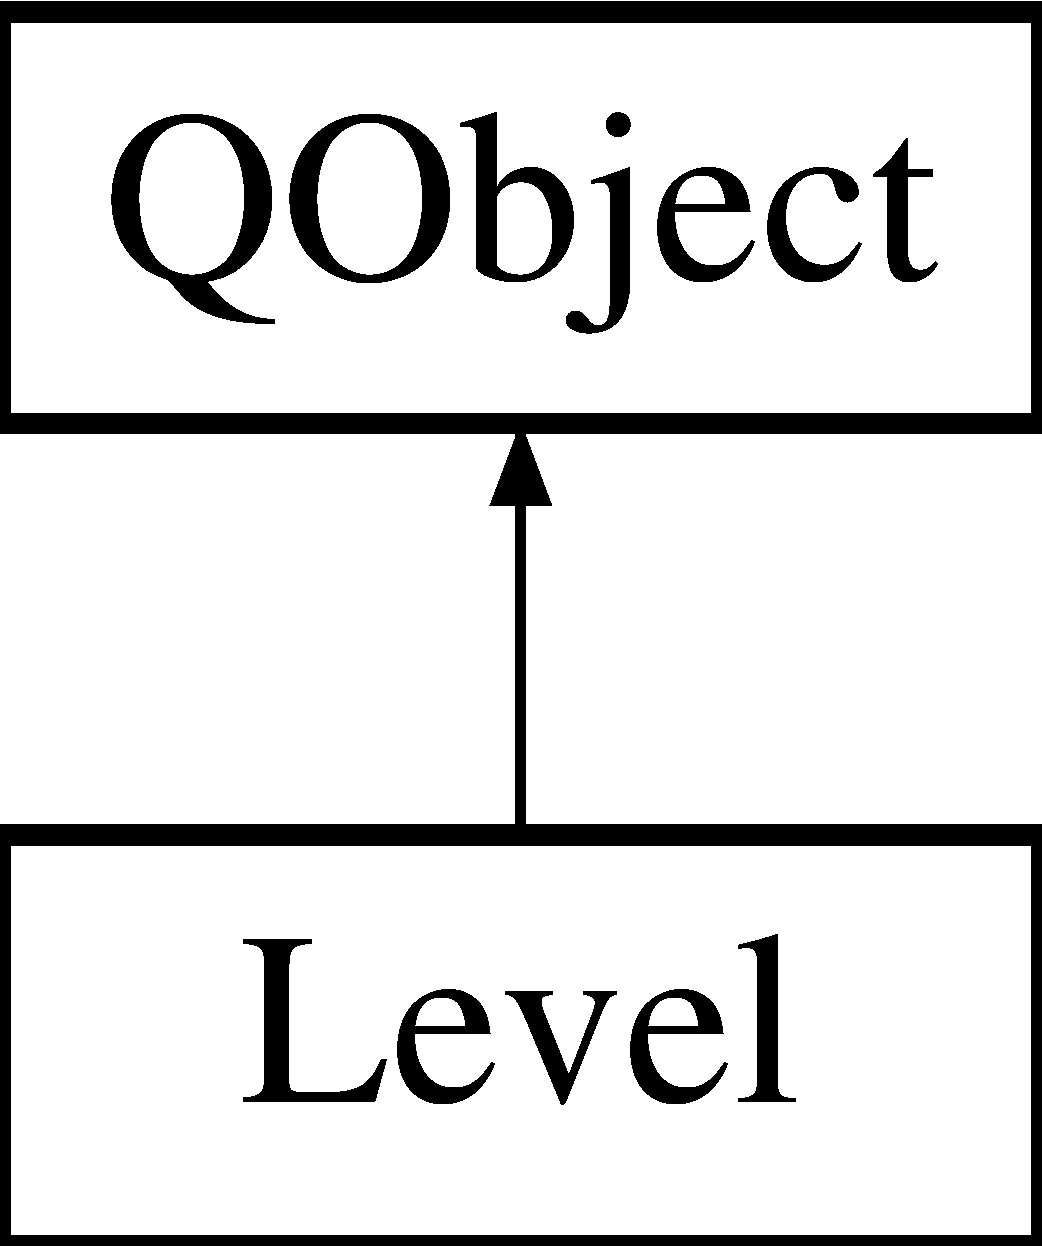
\includegraphics[height=2.000000cm]{class_level}
\end{center}
\end{figure}
\subsection*{Public Slots}
\begin{DoxyCompactItemize}
\item 
\hypertarget{class_level_ab0df304172dc4b1c3965248c4945e776}{}void \hyperlink{class_level_ab0df304172dc4b1c3965248c4945e776}{on\+Energizer\+Eaten} ()\label{class_level_ab0df304172dc4b1c3965248c4945e776}

\begin{DoxyCompactList}\small\item\em Répercute les conséquences d\textquotesingle{}un énergisant sur le mode Appeuré. \end{DoxyCompactList}\item 
\hypertarget{class_level_a4d68a82f73a3519330498c33015bc1a5}{}void \hyperlink{class_level_a4d68a82f73a3519330498c33015bc1a5}{on\+Energizer\+Ending} ()\label{class_level_a4d68a82f73a3519330498c33015bc1a5}

\begin{DoxyCompactList}\small\item\em Démarre le clignotement des fantômes. \end{DoxyCompactList}\item 
\hypertarget{class_level_a8906592d63bc309d535bce9e3af038b6}{}void \hyperlink{class_level_a8906592d63bc309d535bce9e3af038b6}{reverse\+Flash} ()\label{class_level_a8906592d63bc309d535bce9e3af038b6}

\begin{DoxyCompactList}\small\item\em Permet d\textquotesingle{}inverser le flash, faisant clignoter les fantômes. \end{DoxyCompactList}\item 
\hypertarget{class_level_ab44d383ae2a854964e5a991b0c3636ac}{}void \hyperlink{class_level_ab44d383ae2a854964e5a991b0c3636ac}{leave\+Scared\+Move} ()\label{class_level_ab44d383ae2a854964e5a991b0c3636ac}

\begin{DoxyCompactList}\small\item\em Quitte le mode Appeuré. \end{DoxyCompactList}\end{DoxyCompactItemize}
\subsection*{Public Member Functions}
\begin{DoxyCompactItemize}
\item 
\hyperlink{class_level_a610ec153d154322c3d42af030bf54425}{Level} (Q\+Dom\+Element elem)
\begin{DoxyCompactList}\small\item\em Constructeur de base de la classe \hyperlink{class_level}{Level}. \end{DoxyCompactList}\item 
\hyperlink{class_pacman_unit}{Pacman\+Unit} $\ast$ \hyperlink{class_level_afdd877e4e92747abb3718060e77b9cd6}{player} () const 
\begin{DoxyCompactList}\small\item\em Getter. \end{DoxyCompactList}\item 
\hyperlink{class_ghost}{Ghost} \hyperlink{class_level_afe5a9cb5dc0a1f56b5e491298abfc5c5}{ghost} (int ghost\+Idx) const 
\begin{DoxyCompactList}\small\item\em Getter. \end{DoxyCompactList}\item 
void \hyperlink{class_level_a90eaf5382cf0c6a31c0db006644b798c}{set\+Ghosts\+Chasing\+Mode} (int ghosts\+Chasing\+Mode)
\begin{DoxyCompactList}\small\item\em Modifie le comportement des fantômes de ce niveau. \end{DoxyCompactList}\item 
void \hyperlink{class_level_a4ba3695094e42f46ed7af0f489e36b15}{set\+Ghosts\+Scared} (bool scared)
\begin{DoxyCompactList}\small\item\em Active le mode Appeuré des fantômes. \end{DoxyCompactList}\item 
int \hyperlink{class_level_a05f5d955db2a800d9073d5cd9159d6f7}{pellet\+Count} () const 
\begin{DoxyCompactList}\small\item\em Getter. \end{DoxyCompactList}\item 
int \hyperlink{class_level_a22e230e7ff4e40ae092534caafda9060}{eaten\+Pellets} () const 
\begin{DoxyCompactList}\small\item\em Getter. \end{DoxyCompactList}\item 
void \hyperlink{class_level_af6c4d0af3e4e22bb2e543d03e39e68ac}{set\+Eaten\+Pellets} (int \hyperlink{class_level_a22e230e7ff4e40ae092534caafda9060}{eaten\+Pellets})
\begin{DoxyCompactList}\small\item\em Modifie le nombre de pastilles mangées par pacman. \end{DoxyCompactList}\item 
\hyperlink{class_grid}{Grid} $\ast$ \hyperlink{class_level_a61c34c5c6db8f96276fdb87ceaf3d879}{grid} () const 
\begin{DoxyCompactList}\small\item\em Getter. \end{DoxyCompactList}\item 
void \hyperlink{class_level_af43ddfbd5b7b08adc65cf88989280800}{set\+Grid} (\hyperlink{class_grid}{Grid} $\ast$\hyperlink{class_level_a61c34c5c6db8f96276fdb87ceaf3d879}{grid})
\begin{DoxyCompactList}\small\item\em Change de grille utilisée par le niveau. \end{DoxyCompactList}\item 
int \hyperlink{class_level_a870e37a0f1b58e8f0b7beb9819e8cc54}{scared\+Duration} () const 
\begin{DoxyCompactList}\small\item\em Getter. \end{DoxyCompactList}\item 
int \hyperlink{class_level_a002203a9fd3f9ea736af7e940602775c}{flashs\+Count} () const 
\begin{DoxyCompactList}\small\item\em Getter. \end{DoxyCompactList}\item 
void \hyperlink{class_level_a56e0184447f4469d5c13f08577b5c3f9}{set\+Pacman\+Direction} (int direction)
\begin{DoxyCompactList}\small\item\em Tente de modifier la direction du pacman. \end{DoxyCompactList}\item 
Q\+List$<$ \hyperlink{class_ghost}{Ghost} $\ast$ $>$ \hyperlink{class_level_a89da34148d40923b1a1448efd9e68486}{check\+Units\+Positions} ()
\begin{DoxyCompactList}\small\item\em Vérifie si les unités ne se trouvent pas trop proches les unes des autres. \end{DoxyCompactList}\item 
Q\+Image $\ast$ \hyperlink{class_level_a50346e8af1e9b6c6107a104ce70e962e}{render} ()
\begin{DoxyCompactList}\small\item\em Récupère l\textquotesingle{}image de base de la grille et y ajoute les unités. \end{DoxyCompactList}\item 
\hypertarget{class_level_ac61a6b945f5947beed35fea97495c719}{}void \hyperlink{class_level_ac61a6b945f5947beed35fea97495c719}{move\+Pacman} ()\label{class_level_ac61a6b945f5947beed35fea97495c719}

\begin{DoxyCompactList}\small\item\em Calcule le déplacement du pacman du niveau. \end{DoxyCompactList}\item 
\hypertarget{class_level_a16b282122a4046e16e8b28bd1471b933}{}void \hyperlink{class_level_a16b282122a4046e16e8b28bd1471b933}{move\+Ghosts} ()\label{class_level_a16b282122a4046e16e8b28bd1471b933}

\begin{DoxyCompactList}\small\item\em Calcule le déplacement des fantômes du niveau. \end{DoxyCompactList}\item 
\hypertarget{class_level_afb52fc19c9f68243db489df978e142ed}{}void \hyperlink{class_level_afb52fc19c9f68243db489df978e142ed}{update\+Timer} ()\label{class_level_afb52fc19c9f68243db489df978e142ed}

\begin{DoxyCompactList}\small\item\em Met à jour le timer qui gère le mode des fantômes. \end{DoxyCompactList}\item 
\hypertarget{class_level_a8ff7672108dac0debe8d0c0dc1590f34}{}void \hyperlink{class_level_a8ff7672108dac0debe8d0c0dc1590f34}{reset\+Units\+Position} ()\label{class_level_a8ff7672108dac0debe8d0c0dc1590f34}

\begin{DoxyCompactList}\small\item\em Réinitialise la position de toutes unités à leur point de départ. \end{DoxyCompactList}\item 
\hypertarget{class_level_af9979f888060289a08dbc72dc7ab5573}{}void \hyperlink{class_level_af9979f888060289a08dbc72dc7ab5573}{start\+Level} ()\label{class_level_af9979f888060289a08dbc72dc7ab5573}

\begin{DoxyCompactList}\small\item\em Initalise le niveau. \end{DoxyCompactList}\end{DoxyCompactItemize}
\subsection*{Protected Member Functions}
\begin{DoxyCompactItemize}
\item 
void \hyperlink{class_level_ae29473d13944d0ac362d4ab6f7651e29}{add\+Units\+To\+Image} (Q\+Image $\ast$res)
\begin{DoxyCompactList}\small\item\em Ajoute toutes les unités à l\textquotesingle{}image. \end{DoxyCompactList}\item 
void \hyperlink{class_level_afba61ca4ae1267e6b015443d56fdb4dd}{add\+Ghosts\+To\+Image} (Q\+Image $\ast$res)
\begin{DoxyCompactList}\small\item\em Ajoute tous les fantômes à l\textquotesingle{}image. \end{DoxyCompactList}\item 
void \hyperlink{class_level_a973582da2a41b2641cfcfa79d7915b3b}{add\+Pacman\+To\+Image} (Q\+Image $\ast$res)
\begin{DoxyCompactList}\small\item\em Ajoute pacman à l\textquotesingle{}image. \end{DoxyCompactList}\end{DoxyCompactItemize}


\subsection{Detailed Description}
La classe de Niveau de Pacman. 

\begin{DoxyAuthor}{Author}
Valentin D.\+d.\+G. 
\end{DoxyAuthor}
\begin{DoxyVersion}{Version}
1.\+0
\end{DoxyVersion}
Cette classe s\textquotesingle{}occupe des paramètres propres à un seul niveau (Grille, Nombre de pastilles/énergisants, Unités...). 

\subsection{Constructor \& Destructor Documentation}
\hypertarget{class_level_a610ec153d154322c3d42af030bf54425}{}\index{Level@{Level}!Level@{Level}}
\index{Level@{Level}!Level@{Level}}
\subsubsection[{Level(\+Q\+Dom\+Element elem)}]{\setlength{\rightskip}{0pt plus 5cm}Level\+::\+Level (
\begin{DoxyParamCaption}
\item[{Q\+Dom\+Element}]{elem}
\end{DoxyParamCaption}
)}\label{class_level_a610ec153d154322c3d42af030bf54425}


Constructeur de base de la classe \hyperlink{class_level}{Level}. 


\begin{DoxyParams}{Parameters}
{\em elem} & Données X\+M\+L à charger lors de la contruction de l\textquotesingle{}objet.\\
\hline
\end{DoxyParams}
L\textquotesingle{}élément X\+M\+L doit ressembler au template suivant \+:
\begin{DoxyItemize}
\item $<$\hyperlink{class_level}{Level}$>$
\begin{DoxyItemize}
\item $<$\hyperlink{class_grid}{Grid}$>$
\begin{DoxyItemize}
\item $<$Tile\+Count height=\char`\"{}3\char`\"{} width=\char`\"{}3\char`\"{}/$>$
\item $<$Tile\+Size height=\char`\"{}24\char`\"{} width=\char`\"{}24\char`\"{}/$>$
\item $<$Grid\+Values values=\char`\"{}aaacdebbb\char`\"{}/$>$
\item $<$Texture filename=\char`\"{}\+Texture1.\+png\char`\"{}/$>$
\item $<$Texture filename=\char`\"{}\+Texture2.\+png\char`\"{}/$>$
\item $<$Texture filename=\char`\"{}\+Texture\+\_\+\+Pastille.\+png\char`\"{}/$>$
\item $<$Texture filename=\char`\"{}\+Texture\+\_\+\+Energisant.\+png\char`\"{}/$>$
\item $<$Texture filename=\char`\"{}\+Texture\+\_\+\+Vide.\+png\char`\"{}/$>$
\item $<$Collisions\+Grid values=\char`\"{}000111000\char`\"{}/$>$
\item $<$Ghost\+House x=\char`\"{}1\char`\"{} y=\char`\"{}1\char`\"{} width=\char`\"{}1\char`\"{} height=\char`\"{}1\char`\"{}/$>$
\end{DoxyItemize}
\item $<$/ \hyperlink{class_grid}{Grid}$>$
\item $<$Player ix=\char`\"{}0\char`\"{} iy=\char`\"{}0\char`\"{} speed=\char`\"{}77\char`\"{} sspeed = \char`\"{}91\char`\"{} fx = \char`\"{}half\char`\"{}/$>$
\item $<$Blinky ix=\char`\"{}1\char`\"{} iy=\char`\"{}2\char`\"{} speed=\char`\"{}71\char`\"{} sspeed = \char`\"{}50\char`\"{} cornerx=\char`\"{}26\char`\"{} cornery=\char`\"{}-\/2\char`\"{} fx = \char`\"{}half\char`\"{}/$>$
\item $<$Pinky ix=\char`\"{}2\char`\"{} iy=\char`\"{}2\char`\"{} speed=\char`\"{}71\char`\"{} sspeed = \char`\"{}50\char`\"{} cornerx=\char`\"{}2\char`\"{} cornery=\char`\"{}-\/2\char`\"{}/$>$
\item $<$Inky ix=\char`\"{}1\char`\"{} iy=\char`\"{}2\char`\"{} speed=\char`\"{}71\char`\"{} sspeed = \char`\"{}50\char`\"{} cornerx=\char`\"{}28\char`\"{} cornery=\char`\"{}32\char`\"{} fx = \char`\"{}half\char`\"{}/$>$
\item $<$Clyde ix=\char`\"{}2\char`\"{} iy=\char`\"{}2\char`\"{} speed=\char`\"{}71\char`\"{} sspeed = \char`\"{}50\char`\"{} cornerx=\char`\"{}0\char`\"{} cornery=\char`\"{}32\char`\"{}/$>$
\item $<$\hyperlink{class_ghost_timer}{Ghost\+Timer}$>$
\begin{DoxyItemize}
\item $<$Step time=\char`\"{}7\char`\"{} mode=\char`\"{}0\char`\"{}/$>$
\item $<$Step time=\char`\"{}20\char`\"{} mode=\char`\"{}1\char`\"{}/$>$
\item $<$Step time=\char`\"{}7\char`\"{} mode=\char`\"{}0\char`\"{}/$>$
\end{DoxyItemize}
\item $<$/ \hyperlink{class_ghost_timer}{Ghost\+Timer}$>$
\item $<$Scared\+Mode duration=\char`\"{}6000\char`\"{} flashs=\char`\"{}5\char`\"{}/$>$
\end{DoxyItemize}
\item $<$/ \hyperlink{class_level}{Level}$>$ 
\end{DoxyItemize}

\subsection{Member Function Documentation}
\hypertarget{class_level_afba61ca4ae1267e6b015443d56fdb4dd}{}\index{Level@{Level}!add\+Ghosts\+To\+Image@{add\+Ghosts\+To\+Image}}
\index{add\+Ghosts\+To\+Image@{add\+Ghosts\+To\+Image}!Level@{Level}}
\subsubsection[{add\+Ghosts\+To\+Image(\+Q\+Image $\ast$res)}]{\setlength{\rightskip}{0pt plus 5cm}void Level\+::add\+Ghosts\+To\+Image (
\begin{DoxyParamCaption}
\item[{Q\+Image $\ast$}]{res}
\end{DoxyParamCaption}
)\hspace{0.3cm}{\ttfamily [protected]}}\label{class_level_afba61ca4ae1267e6b015443d56fdb4dd}


Ajoute tous les fantômes à l\textquotesingle{}image. 


\begin{DoxyParams}[1]{Parameters}
\mbox{\tt out}  & {\em res} & Image modifiée (passage par pointeur pour éviter la copie). \\
\hline
\end{DoxyParams}
\hypertarget{class_level_a973582da2a41b2641cfcfa79d7915b3b}{}\index{Level@{Level}!add\+Pacman\+To\+Image@{add\+Pacman\+To\+Image}}
\index{add\+Pacman\+To\+Image@{add\+Pacman\+To\+Image}!Level@{Level}}
\subsubsection[{add\+Pacman\+To\+Image(\+Q\+Image $\ast$res)}]{\setlength{\rightskip}{0pt plus 5cm}void Level\+::add\+Pacman\+To\+Image (
\begin{DoxyParamCaption}
\item[{Q\+Image $\ast$}]{res}
\end{DoxyParamCaption}
)\hspace{0.3cm}{\ttfamily [protected]}}\label{class_level_a973582da2a41b2641cfcfa79d7915b3b}


Ajoute pacman à l\textquotesingle{}image. 


\begin{DoxyParams}[1]{Parameters}
\mbox{\tt out}  & {\em res} & Image modifiée (passage par pointeur pour éviter la copie). \\
\hline
\end{DoxyParams}
\hypertarget{class_level_ae29473d13944d0ac362d4ab6f7651e29}{}\index{Level@{Level}!add\+Units\+To\+Image@{add\+Units\+To\+Image}}
\index{add\+Units\+To\+Image@{add\+Units\+To\+Image}!Level@{Level}}
\subsubsection[{add\+Units\+To\+Image(\+Q\+Image $\ast$res)}]{\setlength{\rightskip}{0pt plus 5cm}void Level\+::add\+Units\+To\+Image (
\begin{DoxyParamCaption}
\item[{Q\+Image $\ast$}]{res}
\end{DoxyParamCaption}
)\hspace{0.3cm}{\ttfamily [protected]}}\label{class_level_ae29473d13944d0ac362d4ab6f7651e29}


Ajoute toutes les unités à l\textquotesingle{}image. 


\begin{DoxyParams}[1]{Parameters}
\mbox{\tt out}  & {\em res} & Image modifiée (passage par pointeur pour éviter la copie). \\
\hline
\end{DoxyParams}
\hypertarget{class_level_a89da34148d40923b1a1448efd9e68486}{}\index{Level@{Level}!check\+Units\+Positions@{check\+Units\+Positions}}
\index{check\+Units\+Positions@{check\+Units\+Positions}!Level@{Level}}
\subsubsection[{check\+Units\+Positions()}]{\setlength{\rightskip}{0pt plus 5cm}Q\+List$<$ {\bf Ghost} $\ast$ $>$ Level\+::check\+Units\+Positions (
\begin{DoxyParamCaption}
{}
\end{DoxyParamCaption}
)}\label{class_level_a89da34148d40923b1a1448efd9e68486}


Vérifie si les unités ne se trouvent pas trop proches les unes des autres. 

\begin{DoxyReturn}{Returns}
Liste des fantômes qui sont trop proches de pacman. 
\end{DoxyReturn}
\hypertarget{class_level_a22e230e7ff4e40ae092534caafda9060}{}\index{Level@{Level}!eaten\+Pellets@{eaten\+Pellets}}
\index{eaten\+Pellets@{eaten\+Pellets}!Level@{Level}}
\subsubsection[{eaten\+Pellets() const }]{\setlength{\rightskip}{0pt plus 5cm}int Level\+::eaten\+Pellets (
\begin{DoxyParamCaption}
{}
\end{DoxyParamCaption}
) const}\label{class_level_a22e230e7ff4e40ae092534caafda9060}


Getter. 

\begin{DoxyReturn}{Returns}
Nombre total de pastilles mangées depuis le début du niveau. 
\end{DoxyReturn}
\hypertarget{class_level_a002203a9fd3f9ea736af7e940602775c}{}\index{Level@{Level}!flashs\+Count@{flashs\+Count}}
\index{flashs\+Count@{flashs\+Count}!Level@{Level}}
\subsubsection[{flashs\+Count() const }]{\setlength{\rightskip}{0pt plus 5cm}int Level\+::flashs\+Count (
\begin{DoxyParamCaption}
{}
\end{DoxyParamCaption}
) const}\label{class_level_a002203a9fd3f9ea736af7e940602775c}


Getter. 

\begin{DoxyReturn}{Returns}
Nombre de flashs d\textquotesingle{}avertissement avant fin de l\textquotesingle{}Appeuré. 
\end{DoxyReturn}
\hypertarget{class_level_afe5a9cb5dc0a1f56b5e491298abfc5c5}{}\index{Level@{Level}!ghost@{ghost}}
\index{ghost@{ghost}!Level@{Level}}
\subsubsection[{ghost(int ghost\+Idx) const }]{\setlength{\rightskip}{0pt plus 5cm}{\bf Ghost} Level\+::ghost (
\begin{DoxyParamCaption}
\item[{int}]{ghost\+Idx}
\end{DoxyParamCaption}
) const}\label{class_level_afe5a9cb5dc0a1f56b5e491298abfc5c5}


Getter. 


\begin{DoxyParams}{Parameters}
{\em ghost\+Idx} & Identificateur du fantôme. \\
\hline
\end{DoxyParams}
\begin{DoxyReturn}{Returns}
Fantôme du niveau avec pour identificateur celui donné en paramètre. 
\end{DoxyReturn}
\hypertarget{class_level_a61c34c5c6db8f96276fdb87ceaf3d879}{}\index{Level@{Level}!grid@{grid}}
\index{grid@{grid}!Level@{Level}}
\subsubsection[{grid() const }]{\setlength{\rightskip}{0pt plus 5cm}{\bf Grid} $\ast$ Level\+::grid (
\begin{DoxyParamCaption}
{}
\end{DoxyParamCaption}
) const}\label{class_level_a61c34c5c6db8f96276fdb87ceaf3d879}


Getter. 

\begin{DoxyReturn}{Returns}
Grille du niveau. 
\end{DoxyReturn}
\hypertarget{class_level_a05f5d955db2a800d9073d5cd9159d6f7}{}\index{Level@{Level}!pellet\+Count@{pellet\+Count}}
\index{pellet\+Count@{pellet\+Count}!Level@{Level}}
\subsubsection[{pellet\+Count() const }]{\setlength{\rightskip}{0pt plus 5cm}int Level\+::pellet\+Count (
\begin{DoxyParamCaption}
{}
\end{DoxyParamCaption}
) const}\label{class_level_a05f5d955db2a800d9073d5cd9159d6f7}


Getter. 

\begin{DoxyReturn}{Returns}
Nombre total de pastilles au début du niveau. 
\end{DoxyReturn}
\hypertarget{class_level_afdd877e4e92747abb3718060e77b9cd6}{}\index{Level@{Level}!player@{player}}
\index{player@{player}!Level@{Level}}
\subsubsection[{player() const }]{\setlength{\rightskip}{0pt plus 5cm}{\bf Pacman\+Unit} $\ast$ Level\+::player (
\begin{DoxyParamCaption}
{}
\end{DoxyParamCaption}
) const}\label{class_level_afdd877e4e92747abb3718060e77b9cd6}


Getter. 

\begin{DoxyReturn}{Returns}
Joueur du niveau. 
\end{DoxyReturn}
\hypertarget{class_level_a50346e8af1e9b6c6107a104ce70e962e}{}\index{Level@{Level}!render@{render}}
\index{render@{render}!Level@{Level}}
\subsubsection[{render()}]{\setlength{\rightskip}{0pt plus 5cm}Q\+Image $\ast$ Level\+::render (
\begin{DoxyParamCaption}
{}
\end{DoxyParamCaption}
)}\label{class_level_a50346e8af1e9b6c6107a104ce70e962e}


Récupère l\textquotesingle{}image de base de la grille et y ajoute les unités. 

\begin{DoxyReturn}{Returns}
Image après ajout des unités sur le terrain. 
\end{DoxyReturn}
\hypertarget{class_level_a870e37a0f1b58e8f0b7beb9819e8cc54}{}\index{Level@{Level}!scared\+Duration@{scared\+Duration}}
\index{scared\+Duration@{scared\+Duration}!Level@{Level}}
\subsubsection[{scared\+Duration() const }]{\setlength{\rightskip}{0pt plus 5cm}int Level\+::scared\+Duration (
\begin{DoxyParamCaption}
{}
\end{DoxyParamCaption}
) const}\label{class_level_a870e37a0f1b58e8f0b7beb9819e8cc54}


Getter. 

\begin{DoxyReturn}{Returns}
Temps pendant le lequel un énergisant fait effet (avant les flashs). 
\end{DoxyReturn}
\hypertarget{class_level_af6c4d0af3e4e22bb2e543d03e39e68ac}{}\index{Level@{Level}!set\+Eaten\+Pellets@{set\+Eaten\+Pellets}}
\index{set\+Eaten\+Pellets@{set\+Eaten\+Pellets}!Level@{Level}}
\subsubsection[{set\+Eaten\+Pellets(int eaten\+Pellets)}]{\setlength{\rightskip}{0pt plus 5cm}void Level\+::set\+Eaten\+Pellets (
\begin{DoxyParamCaption}
\item[{int}]{eaten\+Pellets}
\end{DoxyParamCaption}
)}\label{class_level_af6c4d0af3e4e22bb2e543d03e39e68ac}


Modifie le nombre de pastilles mangées par pacman. 


\begin{DoxyParams}{Parameters}
{\em eaten\+Pellets} & Nouveau nombre de pastilles mangées. \\
\hline
\end{DoxyParams}
\hypertarget{class_level_a90eaf5382cf0c6a31c0db006644b798c}{}\index{Level@{Level}!set\+Ghosts\+Chasing\+Mode@{set\+Ghosts\+Chasing\+Mode}}
\index{set\+Ghosts\+Chasing\+Mode@{set\+Ghosts\+Chasing\+Mode}!Level@{Level}}
\subsubsection[{set\+Ghosts\+Chasing\+Mode(int ghosts\+Chasing\+Mode)}]{\setlength{\rightskip}{0pt plus 5cm}void Level\+::set\+Ghosts\+Chasing\+Mode (
\begin{DoxyParamCaption}
\item[{int}]{ghosts\+Chasing\+Mode}
\end{DoxyParamCaption}
)}\label{class_level_a90eaf5382cf0c6a31c0db006644b798c}


Modifie le comportement des fantômes de ce niveau. 


\begin{DoxyParams}{Parameters}
{\em ghosts\+Chasing\+Mode} & Nouveau comportement. \\
\hline
\end{DoxyParams}
\hypertarget{class_level_a4ba3695094e42f46ed7af0f489e36b15}{}\index{Level@{Level}!set\+Ghosts\+Scared@{set\+Ghosts\+Scared}}
\index{set\+Ghosts\+Scared@{set\+Ghosts\+Scared}!Level@{Level}}
\subsubsection[{set\+Ghosts\+Scared(bool scared)}]{\setlength{\rightskip}{0pt plus 5cm}void Level\+::set\+Ghosts\+Scared (
\begin{DoxyParamCaption}
\item[{bool}]{scared}
\end{DoxyParamCaption}
)}\label{class_level_a4ba3695094e42f46ed7af0f489e36b15}


Active le mode Appeuré des fantômes. 


\begin{DoxyParams}{Parameters}
{\em scared} & Si true, active le mode Appeuré, sinon le désactive.\\
\hline
\end{DoxyParams}
(Dés)Active le mode Appeuré et s\textquotesingle{}il n\textquotesingle{}est pas déjà (in)actif, force les fantômes à changer de sens et met à jour leur vitesse. \hypertarget{class_level_af43ddfbd5b7b08adc65cf88989280800}{}\index{Level@{Level}!set\+Grid@{set\+Grid}}
\index{set\+Grid@{set\+Grid}!Level@{Level}}
\subsubsection[{set\+Grid(\+Grid $\ast$grid)}]{\setlength{\rightskip}{0pt plus 5cm}void Level\+::set\+Grid (
\begin{DoxyParamCaption}
\item[{{\bf Grid} $\ast$}]{grid}
\end{DoxyParamCaption}
)}\label{class_level_af43ddfbd5b7b08adc65cf88989280800}


Change de grille utilisée par le niveau. 


\begin{DoxyParams}{Parameters}
{\em grid} & Nouvelle grille. \\
\hline
\end{DoxyParams}
\hypertarget{class_level_a56e0184447f4469d5c13f08577b5c3f9}{}\index{Level@{Level}!set\+Pacman\+Direction@{set\+Pacman\+Direction}}
\index{set\+Pacman\+Direction@{set\+Pacman\+Direction}!Level@{Level}}
\subsubsection[{set\+Pacman\+Direction(int direction)}]{\setlength{\rightskip}{0pt plus 5cm}void Level\+::set\+Pacman\+Direction (
\begin{DoxyParamCaption}
\item[{int}]{direction}
\end{DoxyParamCaption}
)}\label{class_level_a56e0184447f4469d5c13f08577b5c3f9}


Tente de modifier la direction du pacman. 


\begin{DoxyParams}{Parameters}
{\em direction} & Nouvelle direction du pacman. \\
\hline
\end{DoxyParams}


The documentation for this class was generated from the following files\+:\begin{DoxyCompactItemize}
\item 
level.\+h\item 
level.\+cpp\end{DoxyCompactItemize}

\hypertarget{class_pacman_unit}{}\section{Pacman\+Unit Class Reference}
\label{class_pacman_unit}\index{Pacman\+Unit@{Pacman\+Unit}}


Classe de l\textquotesingle{}unité Pacman.  




{\ttfamily \#include $<$pacmanunit.\+h$>$}

Inheritance diagram for Pacman\+Unit\+:\begin{figure}[H]
\begin{center}
\leavevmode
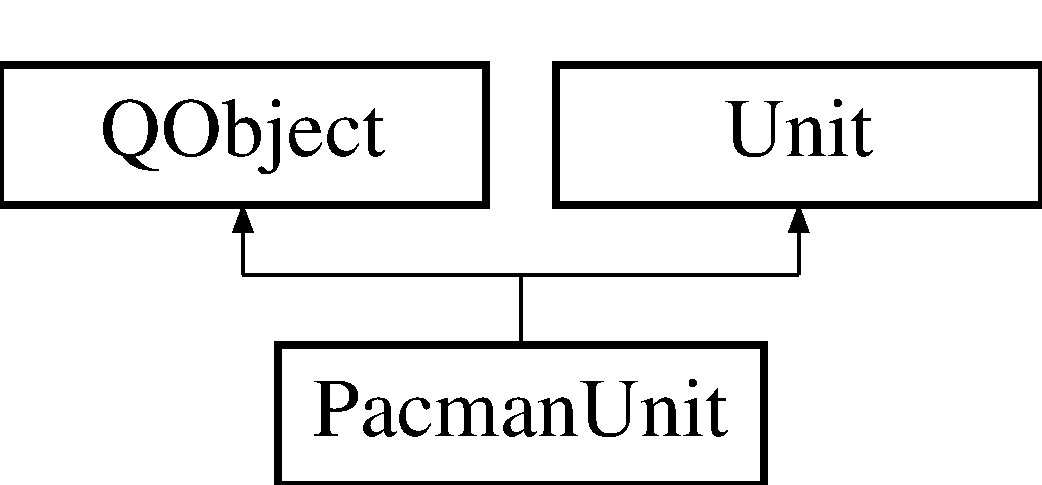
\includegraphics[height=2.000000cm]{class_pacman_unit}
\end{center}
\end{figure}
\subsection*{Signals}
\begin{DoxyCompactItemize}
\item 
\hypertarget{class_pacman_unit_aa1ab8429c64e26cb9b011608f97c9d08}{}void \hyperlink{class_pacman_unit_aa1ab8429c64e26cb9b011608f97c9d08}{pellet\+Eaten} ()\label{class_pacman_unit_aa1ab8429c64e26cb9b011608f97c9d08}

\begin{DoxyCompactList}\small\item\em Emit lorsque le Pacman arrive sur une case avec une pastille. \end{DoxyCompactList}\item 
\hypertarget{class_pacman_unit_a329d9e2c50972a5cae3b4fbd85f83c15}{}void \hyperlink{class_pacman_unit_a329d9e2c50972a5cae3b4fbd85f83c15}{energizer\+Eaten} ()\label{class_pacman_unit_a329d9e2c50972a5cae3b4fbd85f83c15}

\begin{DoxyCompactList}\small\item\em Emit lorsque le Pacman arrive sur une case avec un énergisant. \end{DoxyCompactList}\end{DoxyCompactItemize}
\subsection*{Public Member Functions}
\begin{DoxyCompactItemize}
\item 
\hyperlink{class_pacman_unit_a5da689e1d96160428b625a861cdb7406}{Pacman\+Unit} (Q\+Object $\ast$parent=0)
\begin{DoxyCompactList}\small\item\em Constructeur de base du \hyperlink{class_pacman_unit}{Pacman\+Unit}. \end{DoxyCompactList}\item 
\hyperlink{class_pacman_unit_a5aaebd34aa813060d373a5a80597e4ed}{Pacman\+Unit} (\hyperlink{class_grid}{Grid} $\ast$grid, Q\+Dom\+Element elem, Q\+Object $\ast$parent=0)
\begin{DoxyCompactList}\small\item\em Surcharge du constructeur (avec grille) pour utiliser X\+M\+L. \end{DoxyCompactList}\item 
\hypertarget{class_pacman_unit_afea95a3310aad0ad96f7a22b616e1dc3}{}void \hyperlink{class_pacman_unit_afea95a3310aad0ad96f7a22b616e1dc3}{next\+Frame} ()\label{class_pacman_unit_afea95a3310aad0ad96f7a22b616e1dc3}

\begin{DoxyCompactList}\small\item\em Fait passer le dessin du pacman à la prochain frame (pas de calul d\textquotesingle{}image). \end{DoxyCompactList}\item 
void \hyperlink{class_pacman_unit_a9c4c0c4677e8cda4d9f65d4be17a16f7}{set\+Frame} (int \hyperlink{class_pacman_unit_a55cd713a2c14b16d26c06846598dfbec}{frame})
\begin{DoxyCompactList}\small\item\em Fait directement passer le dessin du pacman à la frame donnée (pas de calul d\textquotesingle{}image). \end{DoxyCompactList}\item 
int \hyperlink{class_pacman_unit_a55cd713a2c14b16d26c06846598dfbec}{frame} () const 
\begin{DoxyCompactList}\small\item\em Getter. \end{DoxyCompactList}\item 
void \hyperlink{class_pacman_unit_a3f5d014178425c2ee077d982ad5f0d7c}{set\+Next\+Direction} (int \hyperlink{class_unit_a5d8a5a789acfa4d2502b0c1082876172}{direction})
\begin{DoxyCompactList}\small\item\em Modifie la prochaine direction que prendra Pacman dès qu\textquotesingle{}il pourra. \end{DoxyCompactList}\item 
\hypertarget{class_pacman_unit_adc791959727ea73b022d37be8d60fa8f}{}void \hyperlink{class_pacman_unit_adc791959727ea73b022d37be8d60fa8f}{move} ()\label{class_pacman_unit_adc791959727ea73b022d37be8d60fa8f}

\begin{DoxyCompactList}\small\item\em Calcule le prochain déplacement du Pacman. \end{DoxyCompactList}\item 
void \hyperlink{class_pacman_unit_a40f1adb4bd0a91b8bef0fb73bd64fb33}{set\+Direction} (int \hyperlink{class_unit_a5d8a5a789acfa4d2502b0c1082876172}{direction})
\begin{DoxyCompactList}\small\item\em Tente de modifier la direction du pacman. \end{DoxyCompactList}\item 
\hypertarget{class_pacman_unit_aedfa1c220c161792b887a5ab75efcaac}{}void \hyperlink{class_pacman_unit_aedfa1c220c161792b887a5ab75efcaac}{reset\+Position} ()\label{class_pacman_unit_aedfa1c220c161792b887a5ab75efcaac}

\begin{DoxyCompactList}\small\item\em Réinitialise la position de Pacman à son origine. \end{DoxyCompactList}\item 
Q\+Pixmap \hyperlink{class_pacman_unit_aeafee04941b0de276151d43480d9d645}{render\+Pacman\+Image} (int size=24)
\begin{DoxyCompactList}\small\item\em Calcule l\textquotesingle{}image de Pacman en fonction de sa direction et de sa frame actuelle. \end{DoxyCompactList}\end{DoxyCompactItemize}
\subsection*{Additional Inherited Members}


\subsection{Detailed Description}
Classe de l\textquotesingle{}unité Pacman. 

\begin{DoxyAuthor}{Author}
Valentin D.\+d.\+G. 
\end{DoxyAuthor}
\begin{DoxyVersion}{Version}
1.\+0
\end{DoxyVersion}
Cette classe héritée de la classe \hyperlink{class_unit}{Unit} permet d\textquotesingle{}ajouter quelques fonctionnalités uniques au Pacman (comme l\textquotesingle{}enregistrement d\textquotesingle{}un coup en avance) ainsi qu\textquotesingle{}une aide pour le dessin du Pacman. 

\subsection{Constructor \& Destructor Documentation}
\hypertarget{class_pacman_unit_a5da689e1d96160428b625a861cdb7406}{}\index{Pacman\+Unit@{Pacman\+Unit}!Pacman\+Unit@{Pacman\+Unit}}
\index{Pacman\+Unit@{Pacman\+Unit}!Pacman\+Unit@{Pacman\+Unit}}
\subsubsection[{Pacman\+Unit(\+Q\+Object $\ast$parent=0)}]{\setlength{\rightskip}{0pt plus 5cm}Pacman\+Unit\+::\+Pacman\+Unit (
\begin{DoxyParamCaption}
\item[{Q\+Object $\ast$}]{parent = {\ttfamily 0}}
\end{DoxyParamCaption}
)}\label{class_pacman_unit_a5da689e1d96160428b625a861cdb7406}


Constructeur de base du \hyperlink{class_pacman_unit}{Pacman\+Unit}. 


\begin{DoxyParams}{Parameters}
{\em parent} & Parent de l\textquotesingle{}objet.\\
\hline
\end{DoxyParams}
Note \+: Cette version du constructeur n\textquotesingle{}est pas destinée à être utilisée en dehors de l\textquotesingle{}initialisation d\textquotesingle{}une classe qui la contient. L\textquotesingle{}objet créé n\textquotesingle{}est pas valide. \hypertarget{class_pacman_unit_a5aaebd34aa813060d373a5a80597e4ed}{}\index{Pacman\+Unit@{Pacman\+Unit}!Pacman\+Unit@{Pacman\+Unit}}
\index{Pacman\+Unit@{Pacman\+Unit}!Pacman\+Unit@{Pacman\+Unit}}
\subsubsection[{Pacman\+Unit(\+Grid $\ast$grid, Q\+Dom\+Element elem, Q\+Object $\ast$parent=0)}]{\setlength{\rightskip}{0pt plus 5cm}Pacman\+Unit\+::\+Pacman\+Unit (
\begin{DoxyParamCaption}
\item[{{\bf Grid} $\ast$}]{grid, }
\item[{Q\+Dom\+Element}]{elem, }
\item[{Q\+Object $\ast$}]{parent = {\ttfamily 0}}
\end{DoxyParamCaption}
)}\label{class_pacman_unit_a5aaebd34aa813060d373a5a80597e4ed}


Surcharge du constructeur (avec grille) pour utiliser X\+M\+L. 


\begin{DoxyParams}{Parameters}
{\em grid} & La grille sur laquelle se trouve Pacman. \\
\hline
{\em elem} & Données X\+M\+L à charger lors de la contruction de l\textquotesingle{}objet. \\
\hline
{\em parent} & \\
\hline
\end{DoxyParams}
Construit un pacman (unité) attaché à une grille et dont les paramètres sont chargés à partir d\textquotesingle{}une balise X\+M\+L.
\begin{DoxyItemize}
\item speed \+: Vitesse par défaut de l\textquotesingle{}unité.
\item sspeed \+: Vitesse lorsque les fantômes sont apeurés.
\item Autres \+: Voir \hyperlink{class_double_position}{Double\+Position(\+Q\+Dom\+Element elem)}.
\end{DoxyItemize}

Exemple \+: $<$Player ix=\char`\"{}14\char`\"{} iy=\char`\"{}23\char`\"{} speed=\char`\"{}77\char`\"{} sspeed = \char`\"{}91\char`\"{} fx = \char`\"{}half\char`\"{}/$>$ 

\subsection{Member Function Documentation}
\hypertarget{class_pacman_unit_a55cd713a2c14b16d26c06846598dfbec}{}\index{Pacman\+Unit@{Pacman\+Unit}!frame@{frame}}
\index{frame@{frame}!Pacman\+Unit@{Pacman\+Unit}}
\subsubsection[{frame() const }]{\setlength{\rightskip}{0pt plus 5cm}int Pacman\+Unit\+::frame (
\begin{DoxyParamCaption}
{}
\end{DoxyParamCaption}
) const}\label{class_pacman_unit_a55cd713a2c14b16d26c06846598dfbec}


Getter. 

\begin{DoxyReturn}{Returns}
Frame actuelle du pacman. 
\end{DoxyReturn}
\hypertarget{class_pacman_unit_aeafee04941b0de276151d43480d9d645}{}\index{Pacman\+Unit@{Pacman\+Unit}!render\+Pacman\+Image@{render\+Pacman\+Image}}
\index{render\+Pacman\+Image@{render\+Pacman\+Image}!Pacman\+Unit@{Pacman\+Unit}}
\subsubsection[{render\+Pacman\+Image(int size=24)}]{\setlength{\rightskip}{0pt plus 5cm}Q\+Pixmap Pacman\+Unit\+::render\+Pacman\+Image (
\begin{DoxyParamCaption}
\item[{int}]{size = {\ttfamily 24}}
\end{DoxyParamCaption}
)}\label{class_pacman_unit_aeafee04941b0de276151d43480d9d645}


Calcule l\textquotesingle{}image de Pacman en fonction de sa direction et de sa frame actuelle. 


\begin{DoxyParams}{Parameters}
{\em size} & Taille de l\textquotesingle{}image résultante. \\
\hline
\end{DoxyParams}
\begin{DoxyReturn}{Returns}
Image du Pacman faisant face dans la direction du Pacman et à la bonne frame. 
\end{DoxyReturn}
\hypertarget{class_pacman_unit_a40f1adb4bd0a91b8bef0fb73bd64fb33}{}\index{Pacman\+Unit@{Pacman\+Unit}!set\+Direction@{set\+Direction}}
\index{set\+Direction@{set\+Direction}!Pacman\+Unit@{Pacman\+Unit}}
\subsubsection[{set\+Direction(int direction)}]{\setlength{\rightskip}{0pt plus 5cm}void Pacman\+Unit\+::set\+Direction (
\begin{DoxyParamCaption}
\item[{int}]{direction}
\end{DoxyParamCaption}
)}\label{class_pacman_unit_a40f1adb4bd0a91b8bef0fb73bd64fb33}


Tente de modifier la direction du pacman. 


\begin{DoxyParams}{Parameters}
{\em direction} & Nouvelle direction.\\
\hline
\end{DoxyParams}
Essaie de modifier la direction actuelle du joueur par le paramètre. Si le joueur ne peut pas effectuer ce mouvement immédiatement, la direction est stockée et sera prise dès que possible. Si une direction est déjà stockée afin d\textquotesingle{}être utilisée dès que possible, elle est écrasée. Si la nouvelle direction est égale à la direction actuelle, la prochaine direction est écrasée (afin d\textquotesingle{}annuler la commande). \hypertarget{class_pacman_unit_a9c4c0c4677e8cda4d9f65d4be17a16f7}{}\index{Pacman\+Unit@{Pacman\+Unit}!set\+Frame@{set\+Frame}}
\index{set\+Frame@{set\+Frame}!Pacman\+Unit@{Pacman\+Unit}}
\subsubsection[{set\+Frame(int frame)}]{\setlength{\rightskip}{0pt plus 5cm}void Pacman\+Unit\+::set\+Frame (
\begin{DoxyParamCaption}
\item[{int}]{frame}
\end{DoxyParamCaption}
)}\label{class_pacman_unit_a9c4c0c4677e8cda4d9f65d4be17a16f7}


Fait directement passer le dessin du pacman à la frame donnée (pas de calul d\textquotesingle{}image). 


\begin{DoxyParams}{Parameters}
{\em frame} & Nouvelle frame du pacman.\\
\hline
\end{DoxyParams}
Utile pour créer un Pacman Dummy afin d\textquotesingle{}afficher une position particulière. \hypertarget{class_pacman_unit_a3f5d014178425c2ee077d982ad5f0d7c}{}\index{Pacman\+Unit@{Pacman\+Unit}!set\+Next\+Direction@{set\+Next\+Direction}}
\index{set\+Next\+Direction@{set\+Next\+Direction}!Pacman\+Unit@{Pacman\+Unit}}
\subsubsection[{set\+Next\+Direction(int direction)}]{\setlength{\rightskip}{0pt plus 5cm}void Pacman\+Unit\+::set\+Next\+Direction (
\begin{DoxyParamCaption}
\item[{int}]{direction}
\end{DoxyParamCaption}
)}\label{class_pacman_unit_a3f5d014178425c2ee077d982ad5f0d7c}


Modifie la prochaine direction que prendra Pacman dès qu\textquotesingle{}il pourra. 


\begin{DoxyParams}{Parameters}
{\em direction} & Nouvelle prochaine direction. \\
\hline
\end{DoxyParams}


The documentation for this class was generated from the following files\+:\begin{DoxyCompactItemize}
\item 
pacmanunit.\+h\item 
pacmanunit.\+cpp\end{DoxyCompactItemize}

\hypertarget{class_pacscreen}{}\section{Pacscreen Class Reference}
\label{class_pacscreen}\index{Pacscreen@{Pacscreen}}


Widget affichant l\textquotesingle{}ensemble du jeu.  




{\ttfamily \#include $<$pacscreen.\+h$>$}

Inheritance diagram for Pacscreen\+:\begin{figure}[H]
\begin{center}
\leavevmode
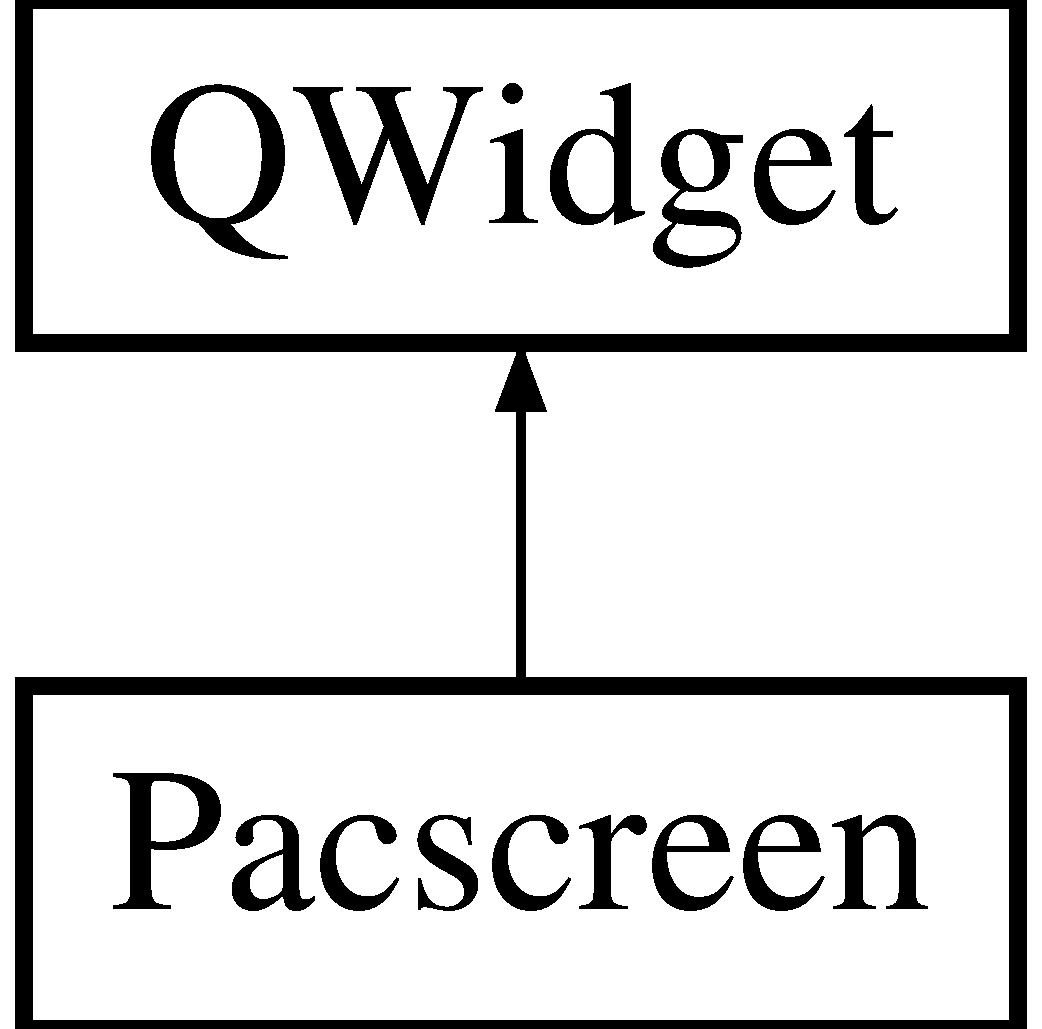
\includegraphics[height=2.000000cm]{class_pacscreen}
\end{center}
\end{figure}
\subsection*{Public Member Functions}
\begin{DoxyCompactItemize}
\item 
\hyperlink{class_pacscreen_a8dfe2adcf7e11f715664859db16c6710}{Pacscreen} (Q\+Widget $\ast$parent=0)
\begin{DoxyCompactList}\small\item\em Constructeur de base de la classe \hyperlink{class_pacscreen}{Pacscreen}. \end{DoxyCompactList}\item 
\hypertarget{class_pacscreen_a4c4bd0bef62cc02bd3798b4d20cd765f}{}\hyperlink{class_pacscreen_a4c4bd0bef62cc02bd3798b4d20cd765f}{$\sim$\+Pacscreen} ()\label{class_pacscreen_a4c4bd0bef62cc02bd3798b4d20cd765f}

\begin{DoxyCompactList}\small\item\em Destructeur de la classe \hyperlink{class_pacscreen}{Pacscreen}. \end{DoxyCompactList}\item 
void \hyperlink{class_pacscreen_a6860cefac4b539818d5d78ace3f61b18}{set\+Game} (\hyperlink{class_game}{Game} $\ast$game)
\begin{DoxyCompactList}\small\item\em Setter. \end{DoxyCompactList}\end{DoxyCompactItemize}
\subsection*{Protected Member Functions}
\begin{DoxyCompactItemize}
\item 
void \hyperlink{class_pacscreen_a487bc9941a204557e94c942a4c95552c}{paint\+Event} (Q\+Paint\+Event $\ast$)
\begin{DoxyCompactList}\small\item\em paint\+Event de la classe, afin d\textquotesingle{}afficher l\textquotesingle{}ensemble du jeu. \end{DoxyCompactList}\end{DoxyCompactItemize}


\subsection{Detailed Description}
Widget affichant l\textquotesingle{}ensemble du jeu. 

\begin{DoxyAuthor}{Author}
Valentin D.\+d.\+G. 
\end{DoxyAuthor}
\begin{DoxyVersion}{Version}
1.\+0
\end{DoxyVersion}
Grâce à l\textquotesingle{}utilisation d\textquotesingle{}un Paint\+Event, cette classe fille de Q\+Widget permet d\textquotesingle{}afficher tous les éléments graphiques du jeu en plein écran.

Cette classe permet aussi de recevoir les commandes utilisateurs venant du clavier ou d\textquotesingle{}une manette Arduino Uno. 

\subsection{Constructor \& Destructor Documentation}
\hypertarget{class_pacscreen_a8dfe2adcf7e11f715664859db16c6710}{}\index{Pacscreen@{Pacscreen}!Pacscreen@{Pacscreen}}
\index{Pacscreen@{Pacscreen}!Pacscreen@{Pacscreen}}
\subsubsection[{Pacscreen(\+Q\+Widget $\ast$parent=0)}]{\setlength{\rightskip}{0pt plus 5cm}Pacscreen\+::\+Pacscreen (
\begin{DoxyParamCaption}
\item[{Q\+Widget $\ast$}]{parent = {\ttfamily 0}}
\end{DoxyParamCaption}
)\hspace{0.3cm}{\ttfamily [explicit]}}\label{class_pacscreen_a8dfe2adcf7e11f715664859db16c6710}


Constructeur de base de la classe \hyperlink{class_pacscreen}{Pacscreen}. 


\begin{DoxyParams}{Parameters}
{\em parent} & Parent de la fenêtre \\
\hline
\end{DoxyParams}


\subsection{Member Function Documentation}
\hypertarget{class_pacscreen_a487bc9941a204557e94c942a4c95552c}{}\index{Pacscreen@{Pacscreen}!paint\+Event@{paint\+Event}}
\index{paint\+Event@{paint\+Event}!Pacscreen@{Pacscreen}}
\subsubsection[{paint\+Event(\+Q\+Paint\+Event $\ast$)}]{\setlength{\rightskip}{0pt plus 5cm}void Pacscreen\+::paint\+Event (
\begin{DoxyParamCaption}
\item[{Q\+Paint\+Event $\ast$}]{}
\end{DoxyParamCaption}
)\hspace{0.3cm}{\ttfamily [protected]}}\label{class_pacscreen_a487bc9941a204557e94c942a4c95552c}


paint\+Event de la classe, afin d\textquotesingle{}afficher l\textquotesingle{}ensemble du jeu. 

Cet évenement est appelé à chaque fois que le timer du Jeu calcule une frame et affiche la frame (il peut y avoir une frame d\textquotesingle{}écart, soit 16-\/17 ms). \hypertarget{class_pacscreen_a6860cefac4b539818d5d78ace3f61b18}{}\index{Pacscreen@{Pacscreen}!set\+Game@{set\+Game}}
\index{set\+Game@{set\+Game}!Pacscreen@{Pacscreen}}
\subsubsection[{set\+Game(\+Game $\ast$game)}]{\setlength{\rightskip}{0pt plus 5cm}void Pacscreen\+::set\+Game (
\begin{DoxyParamCaption}
\item[{{\bf Game} $\ast$}]{game}
\end{DoxyParamCaption}
)}\label{class_pacscreen_a6860cefac4b539818d5d78ace3f61b18}


Setter. 


\begin{DoxyParams}{Parameters}
{\em game} & Jeu à afficher. \\
\hline
\end{DoxyParams}


The documentation for this class was generated from the following files\+:\begin{DoxyCompactItemize}
\item 
pacscreen.\+h\item 
pacscreen.\+cpp\end{DoxyCompactItemize}

\hypertarget{class_texture_handler}{}\section{Texture\+Handler Class Reference}
\label{class_texture_handler}\index{Texture\+Handler@{Texture\+Handler}}


Gestionnaire de textures.  




{\ttfamily \#include $<$texturehandler.\+h$>$}

\subsection*{Public Member Functions}
\begin{DoxyCompactItemize}
\item 
\hyperlink{class_texture_handler_a9056de3d9a44b2e696c8e8b39462dd46}{Texture\+Handler} ()
\begin{DoxyCompactList}\small\item\em Constructeur de base de \hyperlink{class_texture_handler}{Texture\+Handler}. \end{DoxyCompactList}\item 
void \hyperlink{class_texture_handler_a67bc892bd24dfd85bc1eb3af78b8ca40}{add\+Texture} (Q\+String complete\+Filename)
\begin{DoxyCompactList}\small\item\em Ajoute une texture via le chemin du fichier. \end{DoxyCompactList}\item 
Q\+Pixmap \hyperlink{class_texture_handler_a608d66882a46775d1ce498895cf3679b}{texture\+At} (int index) const 
\begin{DoxyCompactList}\small\item\em Getter. \end{DoxyCompactList}\item 
Q\+String \hyperlink{class_texture_handler_a0cdb224be8b1980733698f41b856a55c}{filename\+At} (int index) const 
\begin{DoxyCompactList}\small\item\em Getter. \end{DoxyCompactList}\item 
Q\+String \hyperlink{class_texture_handler_aa6d8737d949687142ffff1e163a15b4f}{texture\+Name\+At} (int index) const 
\begin{DoxyCompactList}\small\item\em Getter. \end{DoxyCompactList}\item 
bool \hyperlink{class_texture_handler_a28014e2b89614335ec2131cdfb94c0be}{contains} (Q\+String filename) const 
\begin{DoxyCompactList}\small\item\em Vérifie si le gestionnaire connait déjà la texture donnée. \end{DoxyCompactList}\item 
int \hyperlink{class_texture_handler_a4753c03df1e7718542557000c04988b1}{index\+Of\+Texture\+Name} (Q\+String texture\+Name) const 
\begin{DoxyCompactList}\small\item\em Récupère l\textquotesingle{}index de la texture dans le gestionnaire. \end{DoxyCompactList}\item 
int \hyperlink{class_texture_handler_aa3fe3f090ff350d2357b4b6fdb570eb7}{count} () const 
\begin{DoxyCompactList}\small\item\em Getter. \end{DoxyCompactList}\item 
int \hyperlink{class_texture_handler_a57242ce71321d2d3376f621486bd432c}{tiles\+Size} () const 
\begin{DoxyCompactList}\small\item\em Getter. \end{DoxyCompactList}\item 
void \hyperlink{class_texture_handler_aecf95d09a430bbc7b92f0a2189b9ff7d}{set\+Tiles\+Size} (int \hyperlink{class_texture_handler_a57242ce71321d2d3376f621486bd432c}{tiles\+Size})
\begin{DoxyCompactList}\small\item\em Setter. \end{DoxyCompactList}\end{DoxyCompactItemize}


\subsection{Detailed Description}
Gestionnaire de textures. 

\begin{DoxyAuthor}{Author}
Valentin D.\+d.\+G. 
\end{DoxyAuthor}
\begin{DoxyVersion}{Version}
1.\+0
\end{DoxyVersion}
Ce gestionnaire de textures permet de faire le lien entre le nom complet d\textquotesingle{}un fichier, son nom en court et son index dans le gestionnaire. Le gestionnaire par défaut modifie la taille des textures. 

\subsection{Constructor \& Destructor Documentation}
\hypertarget{class_texture_handler_a9056de3d9a44b2e696c8e8b39462dd46}{}\index{Texture\+Handler@{Texture\+Handler}!Texture\+Handler@{Texture\+Handler}}
\index{Texture\+Handler@{Texture\+Handler}!Texture\+Handler@{Texture\+Handler}}
\subsubsection[{Texture\+Handler()}]{\setlength{\rightskip}{0pt plus 5cm}Texture\+Handler\+::\+Texture\+Handler (
\begin{DoxyParamCaption}
{}
\end{DoxyParamCaption}
)}\label{class_texture_handler_a9056de3d9a44b2e696c8e8b39462dd46}


Constructeur de base de \hyperlink{class_texture_handler}{Texture\+Handler}. 

Crée un gestionnaire totalement vide. 

\subsection{Member Function Documentation}
\hypertarget{class_texture_handler_a67bc892bd24dfd85bc1eb3af78b8ca40}{}\index{Texture\+Handler@{Texture\+Handler}!add\+Texture@{add\+Texture}}
\index{add\+Texture@{add\+Texture}!Texture\+Handler@{Texture\+Handler}}
\subsubsection[{add\+Texture(\+Q\+String complete\+Filename)}]{\setlength{\rightskip}{0pt plus 5cm}void Texture\+Handler\+::add\+Texture (
\begin{DoxyParamCaption}
\item[{Q\+String}]{complete\+Filename}
\end{DoxyParamCaption}
)}\label{class_texture_handler_a67bc892bd24dfd85bc1eb3af78b8ca40}


Ajoute une texture via le chemin du fichier. 


\begin{DoxyParams}{Parameters}
{\em complete\+Filename} & Chemin complet vers la texture ajoutée. \\
\hline
\end{DoxyParams}
\hypertarget{class_texture_handler_a28014e2b89614335ec2131cdfb94c0be}{}\index{Texture\+Handler@{Texture\+Handler}!contains@{contains}}
\index{contains@{contains}!Texture\+Handler@{Texture\+Handler}}
\subsubsection[{contains(\+Q\+String filename) const }]{\setlength{\rightskip}{0pt plus 5cm}bool Texture\+Handler\+::contains (
\begin{DoxyParamCaption}
\item[{Q\+String}]{filename}
\end{DoxyParamCaption}
) const}\label{class_texture_handler_a28014e2b89614335ec2131cdfb94c0be}


Vérifie si le gestionnaire connait déjà la texture donnée. 


\begin{DoxyParams}{Parameters}
{\em filename} & Chemin complet vers la texture. \\
\hline
\end{DoxyParams}
\begin{DoxyReturn}{Returns}
Vrai si le gestionnaire contient la texture, sinon Faux. 
\end{DoxyReturn}
\hypertarget{class_texture_handler_aa3fe3f090ff350d2357b4b6fdb570eb7}{}\index{Texture\+Handler@{Texture\+Handler}!count@{count}}
\index{count@{count}!Texture\+Handler@{Texture\+Handler}}
\subsubsection[{count() const }]{\setlength{\rightskip}{0pt plus 5cm}int Texture\+Handler\+::count (
\begin{DoxyParamCaption}
{}
\end{DoxyParamCaption}
) const}\label{class_texture_handler_aa3fe3f090ff350d2357b4b6fdb570eb7}


Getter. 

\begin{DoxyReturn}{Returns}
Nombre de textures différentes stockées. 
\end{DoxyReturn}
\hypertarget{class_texture_handler_a0cdb224be8b1980733698f41b856a55c}{}\index{Texture\+Handler@{Texture\+Handler}!filename\+At@{filename\+At}}
\index{filename\+At@{filename\+At}!Texture\+Handler@{Texture\+Handler}}
\subsubsection[{filename\+At(int index) const }]{\setlength{\rightskip}{0pt plus 5cm}Q\+String Texture\+Handler\+::filename\+At (
\begin{DoxyParamCaption}
\item[{int}]{index}
\end{DoxyParamCaption}
) const}\label{class_texture_handler_a0cdb224be8b1980733698f41b856a55c}


Getter. 


\begin{DoxyParams}{Parameters}
{\em index} & Index de la texture dans le gestionnaire. \\
\hline
\end{DoxyParams}
\begin{DoxyReturn}{Returns}
Chemin complet de la texture à l\textquotesingle{}index donné. 
\end{DoxyReturn}
\hypertarget{class_texture_handler_a4753c03df1e7718542557000c04988b1}{}\index{Texture\+Handler@{Texture\+Handler}!index\+Of\+Texture\+Name@{index\+Of\+Texture\+Name}}
\index{index\+Of\+Texture\+Name@{index\+Of\+Texture\+Name}!Texture\+Handler@{Texture\+Handler}}
\subsubsection[{index\+Of\+Texture\+Name(\+Q\+String texture\+Name) const }]{\setlength{\rightskip}{0pt plus 5cm}int Texture\+Handler\+::index\+Of\+Texture\+Name (
\begin{DoxyParamCaption}
\item[{Q\+String}]{texture\+Name}
\end{DoxyParamCaption}
) const}\label{class_texture_handler_a4753c03df1e7718542557000c04988b1}


Récupère l\textquotesingle{}index de la texture dans le gestionnaire. 


\begin{DoxyParams}{Parameters}
{\em texture\+Name} & Nom du fichier de la texture. \\
\hline
\end{DoxyParams}
\begin{DoxyReturn}{Returns}
Index de la texture qui porte le nom donné. 
\end{DoxyReturn}
\hypertarget{class_texture_handler_aecf95d09a430bbc7b92f0a2189b9ff7d}{}\index{Texture\+Handler@{Texture\+Handler}!set\+Tiles\+Size@{set\+Tiles\+Size}}
\index{set\+Tiles\+Size@{set\+Tiles\+Size}!Texture\+Handler@{Texture\+Handler}}
\subsubsection[{set\+Tiles\+Size(int tiles\+Size)}]{\setlength{\rightskip}{0pt plus 5cm}void Texture\+Handler\+::set\+Tiles\+Size (
\begin{DoxyParamCaption}
\item[{int}]{tiles\+Size}
\end{DoxyParamCaption}
)}\label{class_texture_handler_aecf95d09a430bbc7b92f0a2189b9ff7d}


Setter. 


\begin{DoxyParams}{Parameters}
{\em tiles\+Size} & Taille des textures du gestionnaire. \\
\hline
\end{DoxyParams}
\hypertarget{class_texture_handler_a608d66882a46775d1ce498895cf3679b}{}\index{Texture\+Handler@{Texture\+Handler}!texture\+At@{texture\+At}}
\index{texture\+At@{texture\+At}!Texture\+Handler@{Texture\+Handler}}
\subsubsection[{texture\+At(int index) const }]{\setlength{\rightskip}{0pt plus 5cm}Q\+Pixmap Texture\+Handler\+::texture\+At (
\begin{DoxyParamCaption}
\item[{int}]{index}
\end{DoxyParamCaption}
) const}\label{class_texture_handler_a608d66882a46775d1ce498895cf3679b}


Getter. 


\begin{DoxyParams}{Parameters}
{\em index} & Index de la texture dans le gestionnaire. \\
\hline
\end{DoxyParams}
\begin{DoxyReturn}{Returns}
Texture à l\textquotesingle{}index donné. 
\end{DoxyReturn}
\hypertarget{class_texture_handler_aa6d8737d949687142ffff1e163a15b4f}{}\index{Texture\+Handler@{Texture\+Handler}!texture\+Name\+At@{texture\+Name\+At}}
\index{texture\+Name\+At@{texture\+Name\+At}!Texture\+Handler@{Texture\+Handler}}
\subsubsection[{texture\+Name\+At(int index) const }]{\setlength{\rightskip}{0pt plus 5cm}Q\+String Texture\+Handler\+::texture\+Name\+At (
\begin{DoxyParamCaption}
\item[{int}]{index}
\end{DoxyParamCaption}
) const}\label{class_texture_handler_aa6d8737d949687142ffff1e163a15b4f}


Getter. 


\begin{DoxyParams}{Parameters}
{\em index} & Index de la texture dans le gestionnaire. \\
\hline
\end{DoxyParams}
\begin{DoxyReturn}{Returns}
Nom du fichier de la texture à l\textquotesingle{}index donné. 
\end{DoxyReturn}
\hypertarget{class_texture_handler_a57242ce71321d2d3376f621486bd432c}{}\index{Texture\+Handler@{Texture\+Handler}!tiles\+Size@{tiles\+Size}}
\index{tiles\+Size@{tiles\+Size}!Texture\+Handler@{Texture\+Handler}}
\subsubsection[{tiles\+Size() const }]{\setlength{\rightskip}{0pt plus 5cm}int Texture\+Handler\+::tiles\+Size (
\begin{DoxyParamCaption}
{}
\end{DoxyParamCaption}
) const}\label{class_texture_handler_a57242ce71321d2d3376f621486bd432c}


Getter. 

\begin{DoxyReturn}{Returns}
Taille des textures du gestionnaire. 
\end{DoxyReturn}


The documentation for this class was generated from the following files\+:\begin{DoxyCompactItemize}
\item 
texturehandler.\+h\item 
texturehandler.\+cpp\end{DoxyCompactItemize}

\hypertarget{class_unit}{}\section{Unit Class Reference}
\label{class_unit}\index{Unit@{Unit}}


Classe représentant une unité du pacman.  




{\ttfamily \#include $<$unit.\+h$>$}

Inheritance diagram for Unit\+:\begin{figure}[H]
\begin{center}
\leavevmode
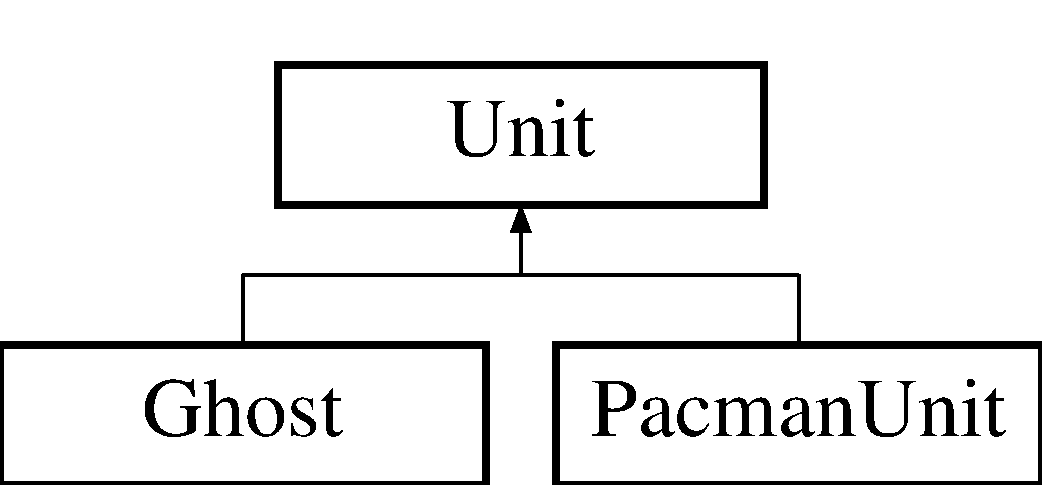
\includegraphics[height=2.000000cm]{class_unit}
\end{center}
\end{figure}
\subsection*{Public Types}
\begin{DoxyCompactItemize}
\item 
enum \hyperlink{class_unit_a198e5fe8c952e2f1e7e9524a914aa0ed}{Directions} \{ \\*
\hyperlink{class_unit_a198e5fe8c952e2f1e7e9524a914aa0edadbae641fa2ba279643d63ee3e071c07a}{Up}, 
\hyperlink{class_unit_a198e5fe8c952e2f1e7e9524a914aa0eda6be5329b08ddd45e62b4d70ae9940f09}{Down}, 
\hyperlink{class_unit_a198e5fe8c952e2f1e7e9524a914aa0eda0d0c9e2b7e0bc40ed55e26b44d2eeae6}{Left}, 
\hyperlink{class_unit_a198e5fe8c952e2f1e7e9524a914aa0eda4b5bae12923642cf30197c5ea676154c}{Right}, 
\\*
\hyperlink{class_unit_a198e5fe8c952e2f1e7e9524a914aa0eda2932642ae5d44019d2d191842b1c818d}{Direction\+Not\+Valid} = -\/1
 \}\begin{DoxyCompactList}\small\item\em Enum des Directions. \end{DoxyCompactList}
\end{DoxyCompactItemize}
\subsection*{Public Member Functions}
\begin{DoxyCompactItemize}
\item 
\hyperlink{class_unit_a8e46f663a95736c8002d85ab271a7581}{Unit} ()
\begin{DoxyCompactList}\small\item\em Constructeur de base de la classe \hyperlink{class_unit}{Unit}. \end{DoxyCompactList}\item 
\hyperlink{class_unit_a581eba4325543aef767722a162ca99cb}{Unit} (\hyperlink{class_grid}{Grid} $\ast$grid)
\begin{DoxyCompactList}\small\item\em Surcharge du constructeur de base référençant la grille. \end{DoxyCompactList}\item 
\hyperlink{class_unit_ab4ca2daa555261d2fa1b8f0edbba667c}{Unit} (\hyperlink{class_grid}{Grid} $\ast$grid, Q\+Dom\+Element elem)
\begin{DoxyCompactList}\small\item\em Surcharge du constructeur (avec grille) pour utiliser X\+M\+L. \end{DoxyCompactList}\item 
Q\+Point \hyperlink{class_unit_a1f96c746ab2d0cc7956e73d59d9c7c70}{position} () const 
\begin{DoxyCompactList}\small\item\em Getter. \end{DoxyCompactList}\item 
Q\+Point \hyperlink{class_unit_a57e72aa7298681d991bf37966d9f2943}{position\+In\+Tile} () const 
\begin{DoxyCompactList}\small\item\em Getter. \end{DoxyCompactList}\item 
\hyperlink{class_double_position}{Double\+Position} \hyperlink{class_unit_a115a97bb5d63670215d42dddc46c9c99}{full\+Position} () const 
\begin{DoxyCompactList}\small\item\em Getter. \end{DoxyCompactList}\item 
void \hyperlink{class_unit_a2424bd74d829e4fc79aa97a083918841}{set\+Direction} (int \hyperlink{class_unit_a5d8a5a789acfa4d2502b0c1082876172}{direction})
\begin{DoxyCompactList}\small\item\em Setter. \end{DoxyCompactList}\item 
int \hyperlink{class_unit_a5d8a5a789acfa4d2502b0c1082876172}{direction} () const 
\begin{DoxyCompactList}\small\item\em Getter. \end{DoxyCompactList}\item 
char \hyperlink{class_unit_a41b1fa4f39ca207da3ad30202b341cd7}{speed} () const 
\begin{DoxyCompactList}\small\item\em Getter. \end{DoxyCompactList}\item 
void \hyperlink{class_unit_aa1b69d788d11e91ed7b9142cfb1bedfb}{set\+Speed} (char \hyperlink{class_unit_a41b1fa4f39ca207da3ad30202b341cd7}{speed})
\begin{DoxyCompactList}\small\item\em Setter. \end{DoxyCompactList}\item 
char \hyperlink{class_unit_a3112ab535d2bf6faef29cb4c4685d43f}{scared\+Speed} () const 
\begin{DoxyCompactList}\small\item\em Getter. \end{DoxyCompactList}\item 
void \hyperlink{class_unit_ae9d92b8ca322719ca8c9a994108d749b}{set\+Scared\+Speed} (char \hyperlink{class_unit_a3112ab535d2bf6faef29cb4c4685d43f}{scared\+Speed})
\begin{DoxyCompactList}\small\item\em Setter. \end{DoxyCompactList}\item 
char \hyperlink{class_unit_a3e8b2e19d807aadc384e5a2092c6bc5c}{base\+Speed} () const 
\begin{DoxyCompactList}\small\item\em Getter. \end{DoxyCompactList}\item 
void \hyperlink{class_unit_a18aa42601bc7e52c2298e87f5ccdd6c5}{set\+Base\+Speed} (char \hyperlink{class_unit_a3e8b2e19d807aadc384e5a2092c6bc5c}{base\+Speed})
\begin{DoxyCompactList}\small\item\em Setter. \end{DoxyCompactList}\item 
void \hyperlink{class_unit_a7b265c0e213164ee5446e6930c0a2155}{reverse\+Speeds} (bool reverse)
\begin{DoxyCompactList}\small\item\em Modifie la vitesse actuelle, soit par celle de base, soit par la vitesse lorsque les fantômes ont peur. \end{DoxyCompactList}\item 
void \hyperlink{class_unit_a3c457eefcea6d9c0e6f07303d4b2f73c}{move\+To\+Tile} (Q\+Point tile)
\begin{DoxyCompactList}\small\item\em Déplace l\textquotesingle{}unité sur la case ciblée. \end{DoxyCompactList}\item 
void \hyperlink{class_unit_ad7e1e0f92908be580fbf75a83fd85467}{move\+To\+Tile} (int \hyperlink{class_unit_a5d8a5a789acfa4d2502b0c1082876172}{direction})
\begin{DoxyCompactList}\small\item\em Déplace l\textquotesingle{}unité sur la prochaine case dans la direction choisie. \end{DoxyCompactList}\item 
void \hyperlink{class_unit_a3ac85960189eb629b56e00ec231b87fa}{move\+To} (int \hyperlink{class_unit_a5d8a5a789acfa4d2502b0c1082876172}{direction})
\begin{DoxyCompactList}\small\item\em Déplace l\textquotesingle{}unité de sa vitesse dans la direction choisie. \end{DoxyCompactList}\item 
void \hyperlink{class_unit_aae1ddaef885741c7b5fc6f1eefd46907}{reset\+Position} ()
\begin{DoxyCompactList}\small\item\em Réinitialise la position de l\textquotesingle{}unité à sa position d\textquotesingle{}origine. \end{DoxyCompactList}\item 
bool \hyperlink{class_unit_a9f26369cc967f76ef91daee0927669aa}{is\+Move\+Legal} (int \hyperlink{class_unit_a5d8a5a789acfa4d2502b0c1082876172}{direction})
\begin{DoxyCompactList}\small\item\em Vérifie si l\textquotesingle{}unité peut se déplacer dans la direction donnée. \end{DoxyCompactList}\end{DoxyCompactItemize}
\subsection*{Static Public Member Functions}
\begin{DoxyCompactItemize}
\item 
static Q\+Point \hyperlink{class_unit_a20108f02c092e52bf4c008a20370b9ef}{direction\+To\+Move} (int \hyperlink{class_unit_a5d8a5a789acfa4d2502b0c1082876172}{direction})
\begin{DoxyCompactList}\small\item\em Calcule l\textquotesingle{}écart selon la direction donnée. \end{DoxyCompactList}\item 
static qreal \hyperlink{class_unit_a4bbd8e88c7b2d16b25067ff2dedcb067}{euclidian\+Distance} (Q\+Point p1, Q\+Point p2)
\begin{DoxyCompactList}\small\item\em Calcule la distance euclidienne d\textquotesingle{}un point à l\textquotesingle{}autre. \end{DoxyCompactList}\end{DoxyCompactItemize}
\subsection*{Protected Attributes}
\begin{DoxyCompactItemize}
\item 
\hypertarget{class_unit_ac4c086ea3b94b3be426c081b33244ca1}{}\hyperlink{class_double_position}{Double\+Position} \hyperlink{class_unit_ac4c086ea3b94b3be426c081b33244ca1}{m\+\_\+position}\label{class_unit_ac4c086ea3b94b3be426c081b33244ca1}

\begin{DoxyCompactList}\small\item\em Position actuelle de l\textquotesingle{}unité \end{DoxyCompactList}\item 
\hypertarget{class_unit_adf868b599517d73750fe30531164f121}{}\hyperlink{class_double_position}{Double\+Position} \hyperlink{class_unit_adf868b599517d73750fe30531164f121}{m\+\_\+origine}\label{class_unit_adf868b599517d73750fe30531164f121}

\begin{DoxyCompactList}\small\item\em Position de base de l\textquotesingle{}unité \end{DoxyCompactList}\item 
\hypertarget{class_unit_a6ef9090f1e7e35c32dc2ad88cb1af761}{}char \hyperlink{class_unit_a6ef9090f1e7e35c32dc2ad88cb1af761}{m\+\_\+direction}\label{class_unit_a6ef9090f1e7e35c32dc2ad88cb1af761}

\begin{DoxyCompactList}\small\item\em Direction actuelle de l\textquotesingle{}unité \end{DoxyCompactList}\item 
\hypertarget{class_unit_a89e65c03176c3485a103c8d74fea84e4}{}char \hyperlink{class_unit_a89e65c03176c3485a103c8d74fea84e4}{m\+\_\+speed}\label{class_unit_a89e65c03176c3485a103c8d74fea84e4}

\begin{DoxyCompactList}\small\item\em Vitesse actuelle de l\textquotesingle{}unité \end{DoxyCompactList}\item 
\hypertarget{class_unit_aa9dff9898710a724a36c04ef55b1eecd}{}char \hyperlink{class_unit_aa9dff9898710a724a36c04ef55b1eecd}{m\+\_\+scared\+Speed}\label{class_unit_aa9dff9898710a724a36c04ef55b1eecd}

\begin{DoxyCompactList}\small\item\em Vitesse de l\textquotesingle{}unité lorsque les fantômes ont peur. \end{DoxyCompactList}\item 
\hypertarget{class_unit_ae7e2ef6ed5459b8783e8698142f6037e}{}char \hyperlink{class_unit_ae7e2ef6ed5459b8783e8698142f6037e}{m\+\_\+base\+Speed}\label{class_unit_ae7e2ef6ed5459b8783e8698142f6037e}

\begin{DoxyCompactList}\small\item\em Vitesse de base de l\textquotesingle{}unité \end{DoxyCompactList}\item 
\hypertarget{class_unit_accaaf0c1e19bf9d254c7c5af96812f34}{}\hyperlink{class_grid}{Grid} $\ast$ \hyperlink{class_unit_accaaf0c1e19bf9d254c7c5af96812f34}{m\+\_\+grid}\label{class_unit_accaaf0c1e19bf9d254c7c5af96812f34}

\begin{DoxyCompactList}\small\item\em Grille sur laquelle circule l\textquotesingle{}unité \end{DoxyCompactList}\end{DoxyCompactItemize}


\subsection{Detailed Description}
Classe représentant une unité du pacman. 

\begin{DoxyAuthor}{Author}
Valentin D.\+d.\+G. 
\end{DoxyAuthor}
\begin{DoxyVersion}{Version}
1.\+0
\end{DoxyVersion}
La classe \hyperlink{class_unit}{Unit} fournit les éléments de base afin de diriger une unité à travers une grille de Pacman. 

\subsection{Member Enumeration Documentation}
\hypertarget{class_unit_a198e5fe8c952e2f1e7e9524a914aa0ed}{}\index{Unit@{Unit}!Directions@{Directions}}
\index{Directions@{Directions}!Unit@{Unit}}
\subsubsection[{Directions}]{\setlength{\rightskip}{0pt plus 5cm}enum {\bf Unit\+::\+Directions}}\label{class_unit_a198e5fe8c952e2f1e7e9524a914aa0ed}


Enum des Directions. 

\begin{Desc}
\item[Enumerator]\par
\begin{description}
\index{Up@{Up}!Unit@{Unit}}\index{Unit@{Unit}!Up@{Up}}\item[{\em 
\hypertarget{class_unit_a198e5fe8c952e2f1e7e9524a914aa0edadbae641fa2ba279643d63ee3e071c07a}{}Up\label{class_unit_a198e5fe8c952e2f1e7e9524a914aa0edadbae641fa2ba279643d63ee3e071c07a}
}]Vers le Haut \index{Down@{Down}!Unit@{Unit}}\index{Unit@{Unit}!Down@{Down}}\item[{\em 
\hypertarget{class_unit_a198e5fe8c952e2f1e7e9524a914aa0eda6be5329b08ddd45e62b4d70ae9940f09}{}Down\label{class_unit_a198e5fe8c952e2f1e7e9524a914aa0eda6be5329b08ddd45e62b4d70ae9940f09}
}]Vers le Bas \index{Left@{Left}!Unit@{Unit}}\index{Unit@{Unit}!Left@{Left}}\item[{\em 
\hypertarget{class_unit_a198e5fe8c952e2f1e7e9524a914aa0eda0d0c9e2b7e0bc40ed55e26b44d2eeae6}{}Left\label{class_unit_a198e5fe8c952e2f1e7e9524a914aa0eda0d0c9e2b7e0bc40ed55e26b44d2eeae6}
}]Vers la Gauche \index{Right@{Right}!Unit@{Unit}}\index{Unit@{Unit}!Right@{Right}}\item[{\em 
\hypertarget{class_unit_a198e5fe8c952e2f1e7e9524a914aa0eda4b5bae12923642cf30197c5ea676154c}{}Right\label{class_unit_a198e5fe8c952e2f1e7e9524a914aa0eda4b5bae12923642cf30197c5ea676154c}
}]Vers la Droite \index{Direction\+Not\+Valid@{Direction\+Not\+Valid}!Unit@{Unit}}\index{Unit@{Unit}!Direction\+Not\+Valid@{Direction\+Not\+Valid}}\item[{\em 
\hypertarget{class_unit_a198e5fe8c952e2f1e7e9524a914aa0eda2932642ae5d44019d2d191842b1c818d}{}Direction\+Not\+Valid\label{class_unit_a198e5fe8c952e2f1e7e9524a914aa0eda2932642ae5d44019d2d191842b1c818d}
}]Direction invalide \end{description}
\end{Desc}


\subsection{Constructor \& Destructor Documentation}
\hypertarget{class_unit_a8e46f663a95736c8002d85ab271a7581}{}\index{Unit@{Unit}!Unit@{Unit}}
\index{Unit@{Unit}!Unit@{Unit}}
\subsubsection[{Unit()}]{\setlength{\rightskip}{0pt plus 5cm}Unit\+::\+Unit (
\begin{DoxyParamCaption}
{}
\end{DoxyParamCaption}
)}\label{class_unit_a8e46f663a95736c8002d85ab271a7581}


Constructeur de base de la classe \hyperlink{class_unit}{Unit}. 

Note \+: Cette version du constructeur n\textquotesingle{}est pas destinée à être utilisée en dehors de l\textquotesingle{}initialisation d\textquotesingle{}une classe qui la contient. L\textquotesingle{}objet créé n\textquotesingle{}est pas valide. \hypertarget{class_unit_a581eba4325543aef767722a162ca99cb}{}\index{Unit@{Unit}!Unit@{Unit}}
\index{Unit@{Unit}!Unit@{Unit}}
\subsubsection[{Unit(\+Grid $\ast$grid)}]{\setlength{\rightskip}{0pt plus 5cm}Unit\+::\+Unit (
\begin{DoxyParamCaption}
\item[{{\bf Grid} $\ast$}]{grid}
\end{DoxyParamCaption}
)}\label{class_unit_a581eba4325543aef767722a162ca99cb}


Surcharge du constructeur de base référençant la grille. 


\begin{DoxyParams}{Parameters}
{\em grid} & La grille sur laquelle se trouve l\textquotesingle{}unité.\\
\hline
\end{DoxyParams}
Une unité créée par ce constructeur est valide mais dispose de tous les paramètres par défaut. \hypertarget{class_unit_ab4ca2daa555261d2fa1b8f0edbba667c}{}\index{Unit@{Unit}!Unit@{Unit}}
\index{Unit@{Unit}!Unit@{Unit}}
\subsubsection[{Unit(\+Grid $\ast$grid, Q\+Dom\+Element elem)}]{\setlength{\rightskip}{0pt plus 5cm}Unit\+::\+Unit (
\begin{DoxyParamCaption}
\item[{{\bf Grid} $\ast$}]{grid, }
\item[{Q\+Dom\+Element}]{elem}
\end{DoxyParamCaption}
)}\label{class_unit_ab4ca2daa555261d2fa1b8f0edbba667c}


Surcharge du constructeur (avec grille) pour utiliser X\+M\+L. 


\begin{DoxyParams}{Parameters}
{\em grid} & La grille sur laquelle se trouve l\textquotesingle{}unité. \\
\hline
{\em elem} & Données X\+M\+L à charger lors de la contruction de l\textquotesingle{}objet.\\
\hline
\end{DoxyParams}
Construit une unité attachée à une grille et dont les paramètres sont chargés à partir d\textquotesingle{}une balise X\+M\+L.
\begin{DoxyItemize}
\item speed \+: Vitesse par défaut de l\textquotesingle{}unité.
\item sspeed \+: Vitesse lorsque les fantômes sont apeurés.
\item Autres \+: Voir \hyperlink{class_double_position}{Double\+Position(\+Q\+Dom\+Element elem)}.
\end{DoxyItemize}

Les vitesses doivent être proches d\textquotesingle{}un multiple de M\+A\+X\+\_\+\+F\+L\+O\+A\+T\+\_\+\+P\+O\+S. Par exemple, avec M\+A\+X\+\_\+\+F\+L\+O\+A\+T\+\_\+\+P\+O\+S égal à 1000, 80 donne un résultat assez éloigné (80$\ast$12 = 960, 80$\ast$13 = 1040) alors que 91 donne une valeur très proche (91$\ast$11 = 1001). Si la valeur est trop éloignée, les unités auront des erreurs dans leur déplacement. De base, l\textquotesingle{}écart maximal absolu est de 25.

A la construction, l\textquotesingle{}élément X\+M\+L doit aussi contenir la position qu\textquotesingle{}aura l\textquotesingle{}unité.

Exemple \+: $<$Player ix=\char`\"{}14\char`\"{} iy=\char`\"{}23\char`\"{} speed=\char`\"{}77\char`\"{} sspeed = \char`\"{}91\char`\"{} fx = \char`\"{}half\char`\"{}/$>$ 

\subsection{Member Function Documentation}
\hypertarget{class_unit_a3e8b2e19d807aadc384e5a2092c6bc5c}{}\index{Unit@{Unit}!base\+Speed@{base\+Speed}}
\index{base\+Speed@{base\+Speed}!Unit@{Unit}}
\subsubsection[{base\+Speed() const }]{\setlength{\rightskip}{0pt plus 5cm}char Unit\+::base\+Speed (
\begin{DoxyParamCaption}
{}
\end{DoxyParamCaption}
) const}\label{class_unit_a3e8b2e19d807aadc384e5a2092c6bc5c}


Getter. 

\begin{DoxyReturn}{Returns}
Vitesse de base de l\textquotesingle{}unité. 
\end{DoxyReturn}
\hypertarget{class_unit_a5d8a5a789acfa4d2502b0c1082876172}{}\index{Unit@{Unit}!direction@{direction}}
\index{direction@{direction}!Unit@{Unit}}
\subsubsection[{direction() const }]{\setlength{\rightskip}{0pt plus 5cm}int Unit\+::direction (
\begin{DoxyParamCaption}
{}
\end{DoxyParamCaption}
) const}\label{class_unit_a5d8a5a789acfa4d2502b0c1082876172}


Getter. 

\begin{DoxyReturn}{Returns}
Direction actuelle de l\textquotesingle{}unité. 
\end{DoxyReturn}
\hypertarget{class_unit_a20108f02c092e52bf4c008a20370b9ef}{}\index{Unit@{Unit}!direction\+To\+Move@{direction\+To\+Move}}
\index{direction\+To\+Move@{direction\+To\+Move}!Unit@{Unit}}
\subsubsection[{direction\+To\+Move(int direction)}]{\setlength{\rightskip}{0pt plus 5cm}Q\+Point Unit\+::direction\+To\+Move (
\begin{DoxyParamCaption}
\item[{int}]{direction}
\end{DoxyParamCaption}
)\hspace{0.3cm}{\ttfamily [static]}}\label{class_unit_a20108f02c092e52bf4c008a20370b9ef}


Calcule l\textquotesingle{}écart selon la direction donnée. 


\begin{DoxyParams}{Parameters}
{\em direction} & Direction de l\textquotesingle{}écart \\
\hline
\end{DoxyParams}
\begin{DoxyReturn}{Returns}
Ecart (norme toujours égale à 1) dans la direction donnée. 
\end{DoxyReturn}
\hypertarget{class_unit_a4bbd8e88c7b2d16b25067ff2dedcb067}{}\index{Unit@{Unit}!euclidian\+Distance@{euclidian\+Distance}}
\index{euclidian\+Distance@{euclidian\+Distance}!Unit@{Unit}}
\subsubsection[{euclidian\+Distance(\+Q\+Point p1, Q\+Point p2)}]{\setlength{\rightskip}{0pt plus 5cm}qreal Unit\+::euclidian\+Distance (
\begin{DoxyParamCaption}
\item[{Q\+Point}]{p1, }
\item[{Q\+Point}]{p2}
\end{DoxyParamCaption}
)\hspace{0.3cm}{\ttfamily [static]}}\label{class_unit_a4bbd8e88c7b2d16b25067ff2dedcb067}


Calcule la distance euclidienne d\textquotesingle{}un point à l\textquotesingle{}autre. 


\begin{DoxyParams}{Parameters}
{\em p1} & Premier point \\
\hline
{\em p2} & Second point \\
\hline
\end{DoxyParams}
\begin{DoxyReturn}{Returns}
Distance euclidienne entre p1 et p2 (valeur réelle)
\end{DoxyReturn}
racine(x1 -\/ x2)$^\wedge$2 + (y1 -\/ y2)$^\wedge$2) \hypertarget{class_unit_a115a97bb5d63670215d42dddc46c9c99}{}\index{Unit@{Unit}!full\+Position@{full\+Position}}
\index{full\+Position@{full\+Position}!Unit@{Unit}}
\subsubsection[{full\+Position() const }]{\setlength{\rightskip}{0pt plus 5cm}{\bf Double\+Position} Unit\+::full\+Position (
\begin{DoxyParamCaption}
{}
\end{DoxyParamCaption}
) const}\label{class_unit_a115a97bb5d63670215d42dddc46c9c99}


Getter. 

\begin{DoxyReturn}{Returns}
\hyperlink{class_double_position}{Double\+Position} de l\textquotesingle{}unité (partie entière et flottante). 
\end{DoxyReturn}
\hypertarget{class_unit_a9f26369cc967f76ef91daee0927669aa}{}\index{Unit@{Unit}!is\+Move\+Legal@{is\+Move\+Legal}}
\index{is\+Move\+Legal@{is\+Move\+Legal}!Unit@{Unit}}
\subsubsection[{is\+Move\+Legal(int direction)}]{\setlength{\rightskip}{0pt plus 5cm}bool Unit\+::is\+Move\+Legal (
\begin{DoxyParamCaption}
\item[{int}]{direction}
\end{DoxyParamCaption}
)}\label{class_unit_a9f26369cc967f76ef91daee0927669aa}


Vérifie si l\textquotesingle{}unité peut se déplacer dans la direction donnée. 


\begin{DoxyParams}{Parameters}
{\em direction} & Direction à vérifier. \\
\hline
\end{DoxyParams}
\begin{DoxyReturn}{Returns}
False si la collision est égale à \hyperlink{class_grid_a473f8c5d768a1734d8911bf1213ce10fa2b394e743be772d4a1da354d5b597623}{Grid\+::\+Collision\+On} sinon True.
\end{DoxyReturn}
La fonction calcule la nouvelle position dans la direction choisie et regarge la collision à cette nouvelle position. Si la collision est On alors on renvoie Faux sinon Vrai.

Note \+: Il est possible d\textquotesingle{}ajouter des types spéciaux de collision, permettant de se déplacer avec de nouvelles valeurs. \hypertarget{class_unit_a3ac85960189eb629b56e00ec231b87fa}{}\index{Unit@{Unit}!move\+To@{move\+To}}
\index{move\+To@{move\+To}!Unit@{Unit}}
\subsubsection[{move\+To(int direction)}]{\setlength{\rightskip}{0pt plus 5cm}void Unit\+::move\+To (
\begin{DoxyParamCaption}
\item[{int}]{direction}
\end{DoxyParamCaption}
)}\label{class_unit_a3ac85960189eb629b56e00ec231b87fa}


Déplace l\textquotesingle{}unité de sa vitesse dans la direction choisie. 


\begin{DoxyParams}{Parameters}
{\em direction} & Direction choisie de déplacement.\\
\hline
\end{DoxyParams}
Déplace l\textquotesingle{}unité de (environ) sa vitesse actuelle dans la direction donnée en paramètre. La valeur est ajoutée/soustraire à la valeur réelle de la position actuelle de l\textquotesingle{}unité.

Si la nouvelle valeur excède la largeur de la grille ou se retrouve sous 0, l\textquotesingle{}unité est déplacée de l\textquotesingle{}autre côté de la grille. \hypertarget{class_unit_a3c457eefcea6d9c0e6f07303d4b2f73c}{}\index{Unit@{Unit}!move\+To\+Tile@{move\+To\+Tile}}
\index{move\+To\+Tile@{move\+To\+Tile}!Unit@{Unit}}
\subsubsection[{move\+To\+Tile(\+Q\+Point tile)}]{\setlength{\rightskip}{0pt plus 5cm}void Unit\+::move\+To\+Tile (
\begin{DoxyParamCaption}
\item[{Q\+Point}]{tile}
\end{DoxyParamCaption}
)}\label{class_unit_a3c457eefcea6d9c0e6f07303d4b2f73c}


Déplace l\textquotesingle{}unité sur la case ciblée. 


\begin{DoxyParams}{Parameters}
{\em tile} & Case cible. \\
\hline
\end{DoxyParams}
\hypertarget{class_unit_ad7e1e0f92908be580fbf75a83fd85467}{}\index{Unit@{Unit}!move\+To\+Tile@{move\+To\+Tile}}
\index{move\+To\+Tile@{move\+To\+Tile}!Unit@{Unit}}
\subsubsection[{move\+To\+Tile(int direction)}]{\setlength{\rightskip}{0pt plus 5cm}void Unit\+::move\+To\+Tile (
\begin{DoxyParamCaption}
\item[{int}]{direction}
\end{DoxyParamCaption}
)}\label{class_unit_ad7e1e0f92908be580fbf75a83fd85467}


Déplace l\textquotesingle{}unité sur la prochaine case dans la direction choisie. 


\begin{DoxyParams}{Parameters}
{\em direction} & Direction choisie de déplacement. \\
\hline
\end{DoxyParams}
\hypertarget{class_unit_a1f96c746ab2d0cc7956e73d59d9c7c70}{}\index{Unit@{Unit}!position@{position}}
\index{position@{position}!Unit@{Unit}}
\subsubsection[{position() const }]{\setlength{\rightskip}{0pt plus 5cm}Q\+Point Unit\+::position (
\begin{DoxyParamCaption}
{}
\end{DoxyParamCaption}
) const}\label{class_unit_a1f96c746ab2d0cc7956e73d59d9c7c70}


Getter. 

\begin{DoxyReturn}{Returns}
Position entière de l\textquotesingle{}unité. 
\end{DoxyReturn}
\hypertarget{class_unit_a57e72aa7298681d991bf37966d9f2943}{}\index{Unit@{Unit}!position\+In\+Tile@{position\+In\+Tile}}
\index{position\+In\+Tile@{position\+In\+Tile}!Unit@{Unit}}
\subsubsection[{position\+In\+Tile() const }]{\setlength{\rightskip}{0pt plus 5cm}Q\+Point Unit\+::position\+In\+Tile (
\begin{DoxyParamCaption}
{}
\end{DoxyParamCaption}
) const}\label{class_unit_a57e72aa7298681d991bf37966d9f2943}


Getter. 

\begin{DoxyReturn}{Returns}
Position réelle de l\textquotesingle{}unité. 
\end{DoxyReturn}
\hypertarget{class_unit_aae1ddaef885741c7b5fc6f1eefd46907}{}\index{Unit@{Unit}!reset\+Position@{reset\+Position}}
\index{reset\+Position@{reset\+Position}!Unit@{Unit}}
\subsubsection[{reset\+Position()}]{\setlength{\rightskip}{0pt plus 5cm}void Unit\+::reset\+Position (
\begin{DoxyParamCaption}
{}
\end{DoxyParamCaption}
)}\label{class_unit_aae1ddaef885741c7b5fc6f1eefd46907}


Réinitialise la position de l\textquotesingle{}unité à sa position d\textquotesingle{}origine. 

Déplace l\textquotesingle{}unité à la position qu\textquotesingle{}il avait lorsqu\textquotesingle{}elle a été créée. \hypertarget{class_unit_a7b265c0e213164ee5446e6930c0a2155}{}\index{Unit@{Unit}!reverse\+Speeds@{reverse\+Speeds}}
\index{reverse\+Speeds@{reverse\+Speeds}!Unit@{Unit}}
\subsubsection[{reverse\+Speeds(bool reverse)}]{\setlength{\rightskip}{0pt plus 5cm}void Unit\+::reverse\+Speeds (
\begin{DoxyParamCaption}
\item[{bool}]{reverse}
\end{DoxyParamCaption}
)}\label{class_unit_a7b265c0e213164ee5446e6930c0a2155}


Modifie la vitesse actuelle, soit par celle de base, soit par la vitesse lorsque les fantômes ont peur. 


\begin{DoxyParams}{Parameters}
{\em reverse} & Si reverse est Vrai alors on utilise la vitesse lorsque les fantômes ont peur, sinon on prend celle de base. \\
\hline
\end{DoxyParams}
\hypertarget{class_unit_a3112ab535d2bf6faef29cb4c4685d43f}{}\index{Unit@{Unit}!scared\+Speed@{scared\+Speed}}
\index{scared\+Speed@{scared\+Speed}!Unit@{Unit}}
\subsubsection[{scared\+Speed() const }]{\setlength{\rightskip}{0pt plus 5cm}char Unit\+::scared\+Speed (
\begin{DoxyParamCaption}
{}
\end{DoxyParamCaption}
) const}\label{class_unit_a3112ab535d2bf6faef29cb4c4685d43f}


Getter. 

\begin{DoxyReturn}{Returns}
Vitesse lorsque les fantômes sont appeurés. 
\end{DoxyReturn}
\hypertarget{class_unit_a18aa42601bc7e52c2298e87f5ccdd6c5}{}\index{Unit@{Unit}!set\+Base\+Speed@{set\+Base\+Speed}}
\index{set\+Base\+Speed@{set\+Base\+Speed}!Unit@{Unit}}
\subsubsection[{set\+Base\+Speed(char base\+Speed)}]{\setlength{\rightskip}{0pt plus 5cm}void Unit\+::set\+Base\+Speed (
\begin{DoxyParamCaption}
\item[{char}]{base\+Speed}
\end{DoxyParamCaption}
)}\label{class_unit_a18aa42601bc7e52c2298e87f5ccdd6c5}


Setter. 


\begin{DoxyParams}{Parameters}
{\em base\+Speed} & Nouvelle vitesse de base de l\textquotesingle{}unité. \\
\hline
\end{DoxyParams}
\hypertarget{class_unit_a2424bd74d829e4fc79aa97a083918841}{}\index{Unit@{Unit}!set\+Direction@{set\+Direction}}
\index{set\+Direction@{set\+Direction}!Unit@{Unit}}
\subsubsection[{set\+Direction(int direction)}]{\setlength{\rightskip}{0pt plus 5cm}void Unit\+::set\+Direction (
\begin{DoxyParamCaption}
\item[{int}]{direction}
\end{DoxyParamCaption}
)}\label{class_unit_a2424bd74d829e4fc79aa97a083918841}


Setter. 


\begin{DoxyParams}{Parameters}
{\em direction} & Nouvelle direction de l\textquotesingle{}unité. \\
\hline
\end{DoxyParams}
\hypertarget{class_unit_ae9d92b8ca322719ca8c9a994108d749b}{}\index{Unit@{Unit}!set\+Scared\+Speed@{set\+Scared\+Speed}}
\index{set\+Scared\+Speed@{set\+Scared\+Speed}!Unit@{Unit}}
\subsubsection[{set\+Scared\+Speed(char scared\+Speed)}]{\setlength{\rightskip}{0pt plus 5cm}void Unit\+::set\+Scared\+Speed (
\begin{DoxyParamCaption}
\item[{char}]{scared\+Speed}
\end{DoxyParamCaption}
)}\label{class_unit_ae9d92b8ca322719ca8c9a994108d749b}


Setter. 


\begin{DoxyParams}{Parameters}
{\em scared\+Speed} & Nouvelle vitesse lorsque les fantômessont appeurés. \\
\hline
\end{DoxyParams}
\hypertarget{class_unit_aa1b69d788d11e91ed7b9142cfb1bedfb}{}\index{Unit@{Unit}!set\+Speed@{set\+Speed}}
\index{set\+Speed@{set\+Speed}!Unit@{Unit}}
\subsubsection[{set\+Speed(char speed)}]{\setlength{\rightskip}{0pt plus 5cm}void Unit\+::set\+Speed (
\begin{DoxyParamCaption}
\item[{char}]{speed}
\end{DoxyParamCaption}
)}\label{class_unit_aa1b69d788d11e91ed7b9142cfb1bedfb}


Setter. 


\begin{DoxyParams}{Parameters}
{\em speed} & Nouvelle vitesse actuelle de l\textquotesingle{}unité. \\
\hline
\end{DoxyParams}
\hypertarget{class_unit_a41b1fa4f39ca207da3ad30202b341cd7}{}\index{Unit@{Unit}!speed@{speed}}
\index{speed@{speed}!Unit@{Unit}}
\subsubsection[{speed() const }]{\setlength{\rightskip}{0pt plus 5cm}char Unit\+::speed (
\begin{DoxyParamCaption}
{}
\end{DoxyParamCaption}
) const}\label{class_unit_a41b1fa4f39ca207da3ad30202b341cd7}


Getter. 

\begin{DoxyReturn}{Returns}
Vitesse actuelle de l\textquotesingle{}unité. 
\end{DoxyReturn}


The documentation for this class was generated from the following files\+:\begin{DoxyCompactItemize}
\item 
unit.\+h\item 
unit.\+cpp\end{DoxyCompactItemize}

%--- End generated contents ---

% Index
\backmatter
\newpage
\phantomsection
\clearemptydoublepage
\addcontentsline{toc}{chapter}{Index}
\printindex

\end{document}
